

\documentclass{article}
\usepackage{anyfontsize}
\usepackage{graphicx}
\usepackage{hyperref}
\usepackage{parskip}
\usepackage{enumitem}
\usepackage{array}
\usepackage{tabularx}
\usepackage[section]{placeins}
\usepackage{float}% If comment this, figure moves to Page 2
\usepackage[dvipsnames]{xcolor}
\usepackage{listings}
\usepackage{alloy-style}

\fontsize{10pt}{12pt}\selectfont % Set the font size
\begin{document}

% FRONT PAGE
\begin{titlepage}
    \begin{center}
        
        Politecnico di Milano\\
      
        Computer Science and Engineering\\
        
        Software Engineering II\\

        \vfill
        
        {\Large \textbf{Design Document - CodeKataBlade}}\\
        
        \vfill

        José Alejandro Sarmiento

        \today

        v1.0
        
    \end{center}
\end{titlepage}
\newpage


% TABLE OF CONTENTS
\tableofcontents
\newpage

% 1. INTRODUCTION
\section{INTRODUCTION}
\subsection{Purpose}

The purpose of this document is to provide a detailed description of the architecture of the system to be, CodeKataBlade, and to show how the requirements presented in the RASD document are met by the architecture. The document also contains the implementation, integration and test plan for the system.

\subsection{Scope}

CodeKataBlade is a software system designed to facilitate and enhance the practice of code katas, which are small coding exercises aimed at improving programming skills. The system provides a platform where educators can create tournaments and battles, and students can register, form teams, and submit their solutions to coding problems.

CodeKataBlade allows educators to create tournaments, which serve as spaces for organizing multiple battles. Educators can invite other educators to participate in tournaments and perform manual evaluations on the submissions of battles they own. The system also provides a leaderboard that is updated in real-time, displaying the rankings of participants based on their performance in the battles.

Students can register to tournaments and battles, either individually or as part of a team. They can submit their solutions to coding problems within the specified deadlines. The system automatically evaluates the submissions using build automation scripts and provides feedback to the students. A set of test cases is used to assess the correctness and efficiency of the solutions.

CodeKataBlade integrates with GitHub, a popular code hosting platform, allowing students to fork repositories and work on their solutions using version control. GitHub Actions, a CI/CD tool, is utilized to automate the evaluation process and provide continuous integration and delivery capabilities.

\subsection{Definitions, Acronyms, Abbreviations}

\subsubsection{Definitions}
 
\begin{itemize}
    \item \textbf{Tournament:} A tournament is a space where educators can create battles and students can register to them. It has a registration deadline and a leaderboard that is updated every time a battle ends.
    \item \textbf{Battle:} A battle is a space where students can register to and submit their solutions to a problem. It has a registration deadline, a final submission deadline, a leaderboard that is updated every time a new evaluation is performed and a set of test cases that will be used to evaluate the submissions.
    \item \textbf{GitHub:} GitHub is a code hosting platform for version control and collaboration. It lets you and others work together on projects from anywhere.
    \item \textbf{GitHub Actions:} GitHub Actions is a CI/CD tool that allows you to automate your software development workflows in the same place you store code and collaborate on pull requests and issues.
    \item \textbf{Educator:} An educator, in the context of the system, is a user of the platform that can create tournaments and battles, invite other educators to tournaments, perform manual evaluations on the submissions of a battle they own and consolidate the results of a battle.
    \item \textbf{Student:} A student, in the context of the system, is a user of the platform that can register to tournaments and battles, create teams and submit their solutions to a battle.
    \item \textbf{Build Automation Scripts:} Build automation scripts are scripts that are run automatically by the system every time a commit is pushed to the main branch of the forked repository of a battle. They are used to evaluate the submissions of the students.
    \item \textbf{Test Case:} A test case is a set of conditions under which a tester will determine whether an application, software system or one of its features is working as it was originally established for it to do.
    \item \textbf{Timeliness:} Timeliness is the quality of doing something or producing something at the right time. In the context of the system, it refers to the time in which a student submits their solution to a battle with respect to the start of the battle and the final submission deadline.
\end{itemize}

\subsubsection{Acronyms}

\begin{itemize}
    \item \textbf{CKB:} CodeKataBattle
    \item \textbf{S2B:} System to Be
    \item \textbf{TDD:} Test-Driven Development
    \item \textbf{CI/CD:} Continuous Integration/Continuous Delivery
    \item \textbf{UI:} User Interface
    \item \textbf{API:} Application Programming Interface
    \item \textbf{UML:} Unified Modeling Language
\end{itemize}

\subsubsection{Abbreviations}

\begin{itemize}
    \item \textbf{Gn:} Goal number n
    \item \textbf{Wn:} World Phenomena number n
    \item \textbf{SPn:} Shared Phenomena number n
    \item \textbf{Dn:} Domain Assumption number n
    \item \textbf{Rn:} Requirement number 
    \item \textbf{UCn:} Use Case number n
\end{itemize}

\subsection{Revision history}
\subsection{Reference Documents}

The specification of the RASD and DD assignment of the Software
Engineering II course, held by professor Matteo Rossi, Elisabetta Di Nitto and
Matteo Camilli at the Politecnico di Milano, A.Y 2023/2024.

\subsection{Document Structure}

\begin{itemize}
    \item \textbf{1. Introduction:} This section provides an overview of the entire document. It describes the purpose and scope of the system, the definitions, acronyms and abbreviations used in the document, the revision history and the reference documents.
    \item \textbf{2. Architectural Design:} This section describes the architecture of the system. It provides an overview of the high-level components and their interaction, the component view, the deployment view, the runtime view, the component interfaces, the selected architectural styles and patterns and other design decisions.
    \item \textbf{3. User Interface Design:} This section provides a mockup of the user interface of the system.
    \item \textbf{4. Requirements Traceability:} This section describes how the requirements defined in the RASD map to the design elements defined in this document.
    \item \textbf{5. Implementation, Integration and Test Plan:} This section describes the order in which the components of the system will be implemented, integrated and tested.
    \item \textbf{6. Effort Spent:} This section describes the amount of time spent by each group member to redact this document.
    \item \textbf{7. References:} This section provides a list of the reference documents used to redact this document. 
\end{itemize}

% 2. ARCHITECTURAL DESIGN
\section{ARCHITECTURAL DESIGN}
\subsection{Overview: High-level components and their interaction}

\begin{figure}[H]
    \centering
    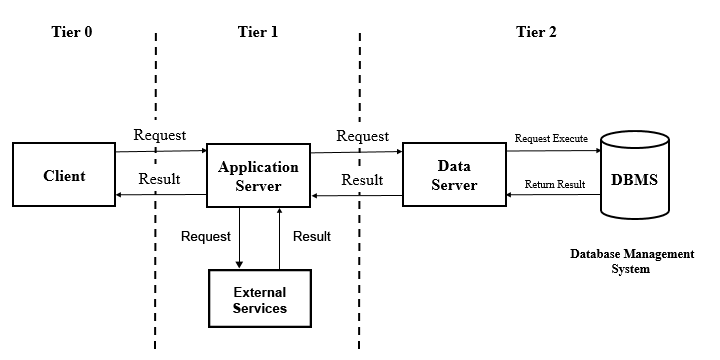
\includegraphics[width=1\textwidth]{images/3-tier-architecture.png}
    \caption{Three-tier Architecture}
    \label{fig:3-tier-architecture}
\end{figure}
The chosen architecture for the system is a three-tier architecture, a widely adopted
model for developing scalable and maintainable web applications. This architectural 
style divides the application into three interconnected layers: presentation, application, 
and data, with the addition of the external services like GitHub and email services.
The rationale behind selecting this architecture is to achieve separation of concerns, 
modularity, and scalability.

\subsubsection*{Presentation Layer}

The presentation layer constitutes the user interfaces for both students and educators, 
encompassing web or mobile interfaces. It is responsible for user interactions, 
displaying data, and triggering actions within the system.

\subsubsection*{Application Layer}

The application layer serves as the business logic layer, managing core functionalities 
such as user authentication, tournament and battle processes, submissions, and evaluations. 
It facilitates bidirectional communication with both the presentation layer and the data layer.

\subsubsection*{Data Layer}

The data layer, comprising the database and external services, handles the storage and 
retrieval of persistent data. It communicates with the application layer to respond to data 
requests, ensuring efficient data management.


% Interaction
\subsubsection{Interaction}
The interaction between the components is as follows:

% Presentation Layer and Application Layer
\subsubsection*{Presentation Layer and Application Layer}
The presentation layer communicates with the application layer through well-defined APIs. This interaction handles user inputs and actions, ensuring a smooth user experience.

% Application Layer and Data Layer
\subsubsection*{Application Layer and Data Layer}
The application layer interacts with the data layer to fetch or store information in the database. This interaction ensures that the platform has access to the necessary data for its operation.

% Application Layer and External Components
\subsubsection*{Application Layer and External Components}
External services, such as the GitHub API for code repositories and an email service for notifications, are integrated into the application layer. This interaction enhances the platform's functionality by incorporating external features.

\subsubsection{Advantages of Three-Tier Architecture}

\begin{itemize}
    \item \textbf{Loose Coupling:} Separation of layers promotes loose coupling, enhancing 
    modularity and ease of maintenance.
    \item \textbf{Scalability:} Each layer can be independently scaled based on specific 
    requirements, allowing for better performance and resource utilization.
\end{itemize}

\newpage

\subsection{Component view}

\begin{figure}[H]
    \centering
    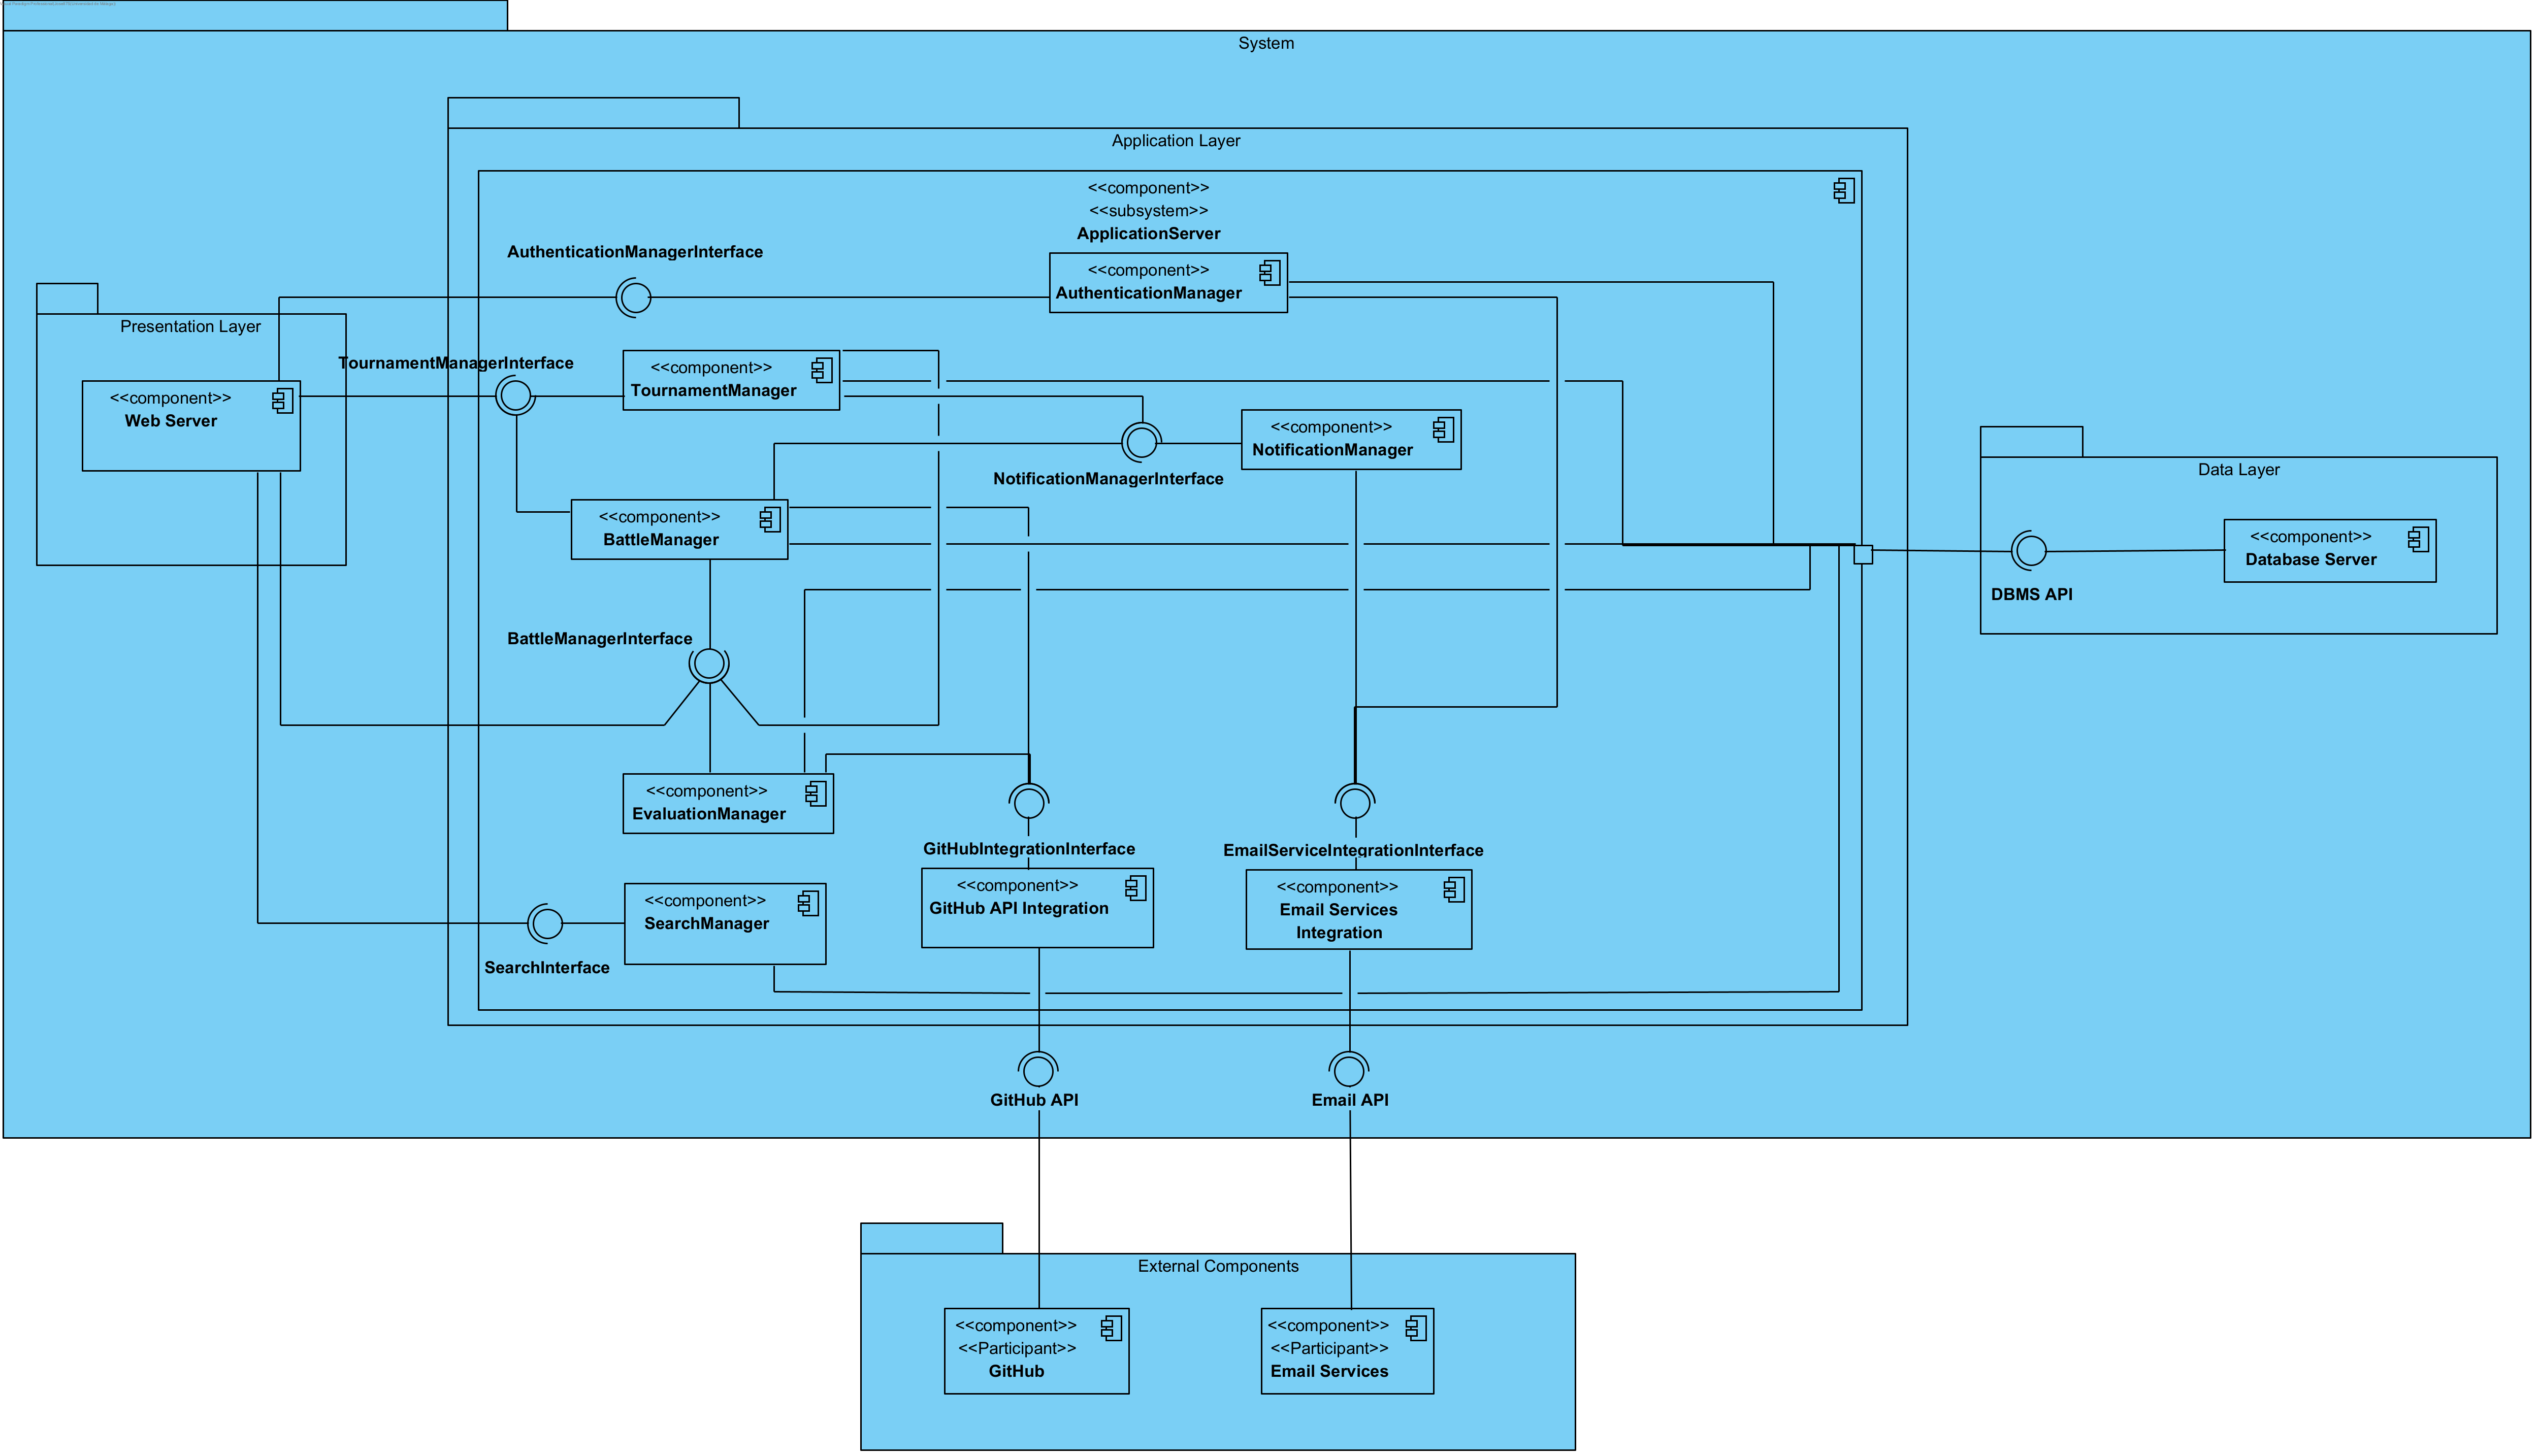
\includegraphics[width=1\textwidth]{images/ComponentDiagram.png}
    \caption{Component Diagram}
    \label{fig:ComponentDiagram}
\end{figure}

\subsubsection{Presentation Layer}

\paragraph{Web Application:}

\begin{itemize}
    \item Represents the web application that will be used by educators and students.
    \item Allows educators to create tournaments and battles, invite other educators to tournaments, and perform manual evaluations on the submissions of battles they own.
    \item Allows students to register to tournaments and battles, create teams, and submit their solutions to battles.
    \item Provides a leaderboard that is updated in real-time, displaying the rankings of participants based on their performance in the battles.
    \item Provides a search functionality that allows users to search for tournaments and battles.
    \item Interfaces with the Web Server for communication with the Application Layer.
\end{itemize}

\paragraph{Web Server:}

\begin{itemize}
    \item Represents the component responsible for hosting the web application.
    \item Handles requests and responses from all users, including educators and students.
    \item Invokes APIs for communication with the Application Layer.
\end{itemize}

\subsubsection{Application Layer}

\paragraph{AuthenticationManager:}

\begin{itemize}
    \item Manages user authentication for educators and students.
    \item Generates and validates authentication tokens.
    \item Interfaces with email services for account confirmation and recovery.
    \item Interfaces with the Data Layer for user authentication.
\end{itemize}

\paragraph{TournamentManager:}

\begin{itemize}
    \item Manages the creation, moderation, and deletion of tournaments.
    \item Handles tournament-related processes and rules.
    \item Interfaces with the NotificationManager for tournament-related notifications.
    \item Interfaces with the Data Layer for tournament data.
\end{itemize}

\paragraph{BattleManager:}

\begin{itemize}
    \item Manages the creation, moderation, and deletion of battles within tournaments.
    \item Handles battle-related processes such as registrations, its deadlines, its GitHub 
    repository creation, and its leaderboard.
    \item Interfaces with the TournamentManager for tournament-related processes such as tournament leadeboard updating.
    \item Interfaces with the NotificationManager for battle-related notifications.
    \item Interfaces with GitHub API Integration for repository creation.
    \item Interfaces with the Data Layer for battle data.
\end{itemize}

\paragraph{EvaluationManager:}

\begin{itemize}
    \item Handles the evaluation of code submissions based on set criteria.
    \item Utilizes build automation scripts and test cases for evaluation.
    \item Interfaces with GitHub API Integration for repository pulling.
    \item Interfaces with the Data Layer for storage of evaluation results.
    \item Has a port through which it receives messages from GitHub which are called during GitHub Actions on submissions and evaluations.
\end{itemize}

\paragraph{NotificationManager:}

\begin{itemize}
    \item Manages the sending of notifications to users.
    \item Interfaces with Email Services Integration for sending notifications via email.
\end{itemize}

\paragraph{SearchManager:}

\begin{itemize}
    \item Manages the search functionality of the platform.
    \item Allows users to search for tournaments and battles.
    \item Interfaces with the Data Layer for tournament and battle data.
\end{itemize}

\subsubsection*{External Components Integration}

\paragraph{GitHub API Integration:}

\begin{itemize}
    \item Interacts with the EvaluationManager to notify of new submissions.
    \item Communicates with the external GitHub API for repository creation and pulling.
\end{itemize}

\paragraph{Email Services Integration:}

\begin{itemize}
    \item Integrates with Email Services for sending notifications.
    \item Sends notifications for tournament invitations, submission updates, etc.
    \item Communicates with the external Email Services API for sending emails.
\end{itemize}

\subsubsection{Data Layer}

\paragraph{Database:}

\begin{itemize}
    \item Manages the storage and retrieval of persistent data.
    \item Stores information related to tournaments, battles, users, submissions, etc.
\end{itemize}


\subsection{Deployment view}

\begin{figure}[H]
    \centering
    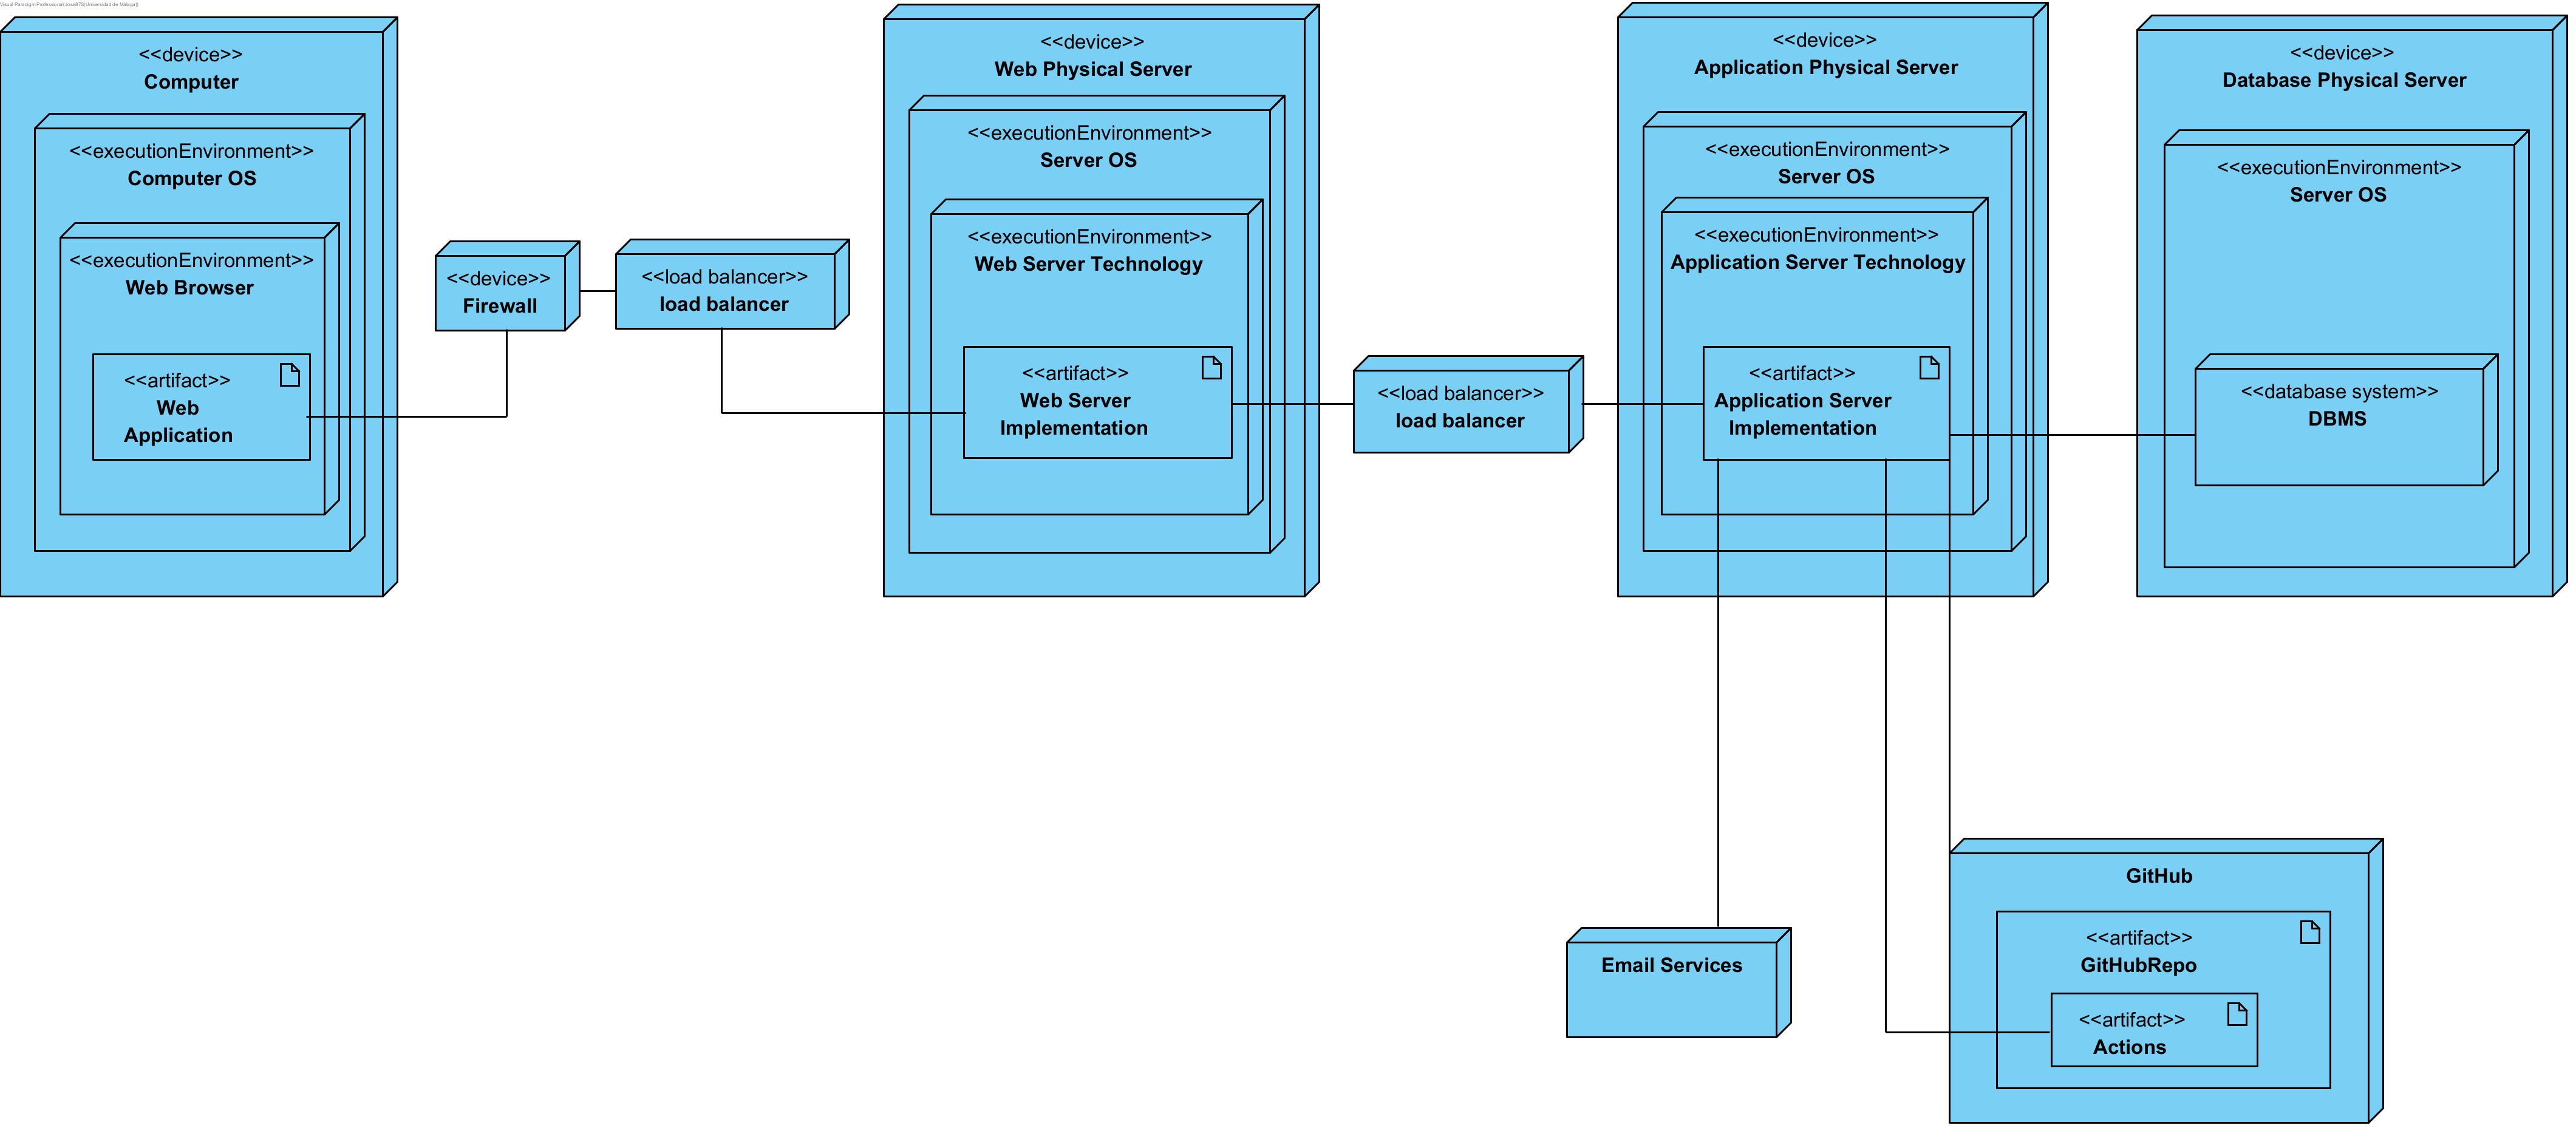
\includegraphics[width=1\textwidth]{images/DeploymentDiagram.png}
    \caption{Deployment Diagram}
    \label{fig:DeploymentDiagram}
\end{figure}

On the deployment diagram, we can see the different components of the system and how they are 
deployed on the different nodes. In this case, the shown deployment assumes the application is developed on Java.
The web application runs on the users' PC which communicates with the
web server, which runs on a Web Server Technology which could be Apache Tomcat, Nginx or other. This two 
elements represent the presentation layer.
The web server is connected to the application server, which runs on a Java EE Application Server. This
element represents the application layer. The application server is connected to the database and to 
the external components. The database is managed by a Database Management System such as MySQL, PostgreSQL or other. 

\newpage

\subsection{Runtime view}

In the following diagrams we can see the sequence diagrams of the main functionalities of the system.
These are more fleshed out versions of the use case diagrams presented in the RASD document. It is important to 
note that the calls to the database server are just not depicted as they would in a real scenario, since these
are normally done via queries and not via custom method calls. It was represented via method calls so that
it is easier to understand the meaning calls to the database server and the parameters used.

\subsubsection*{UC1 - Login}

\begin{figure}[H]
    \centering
    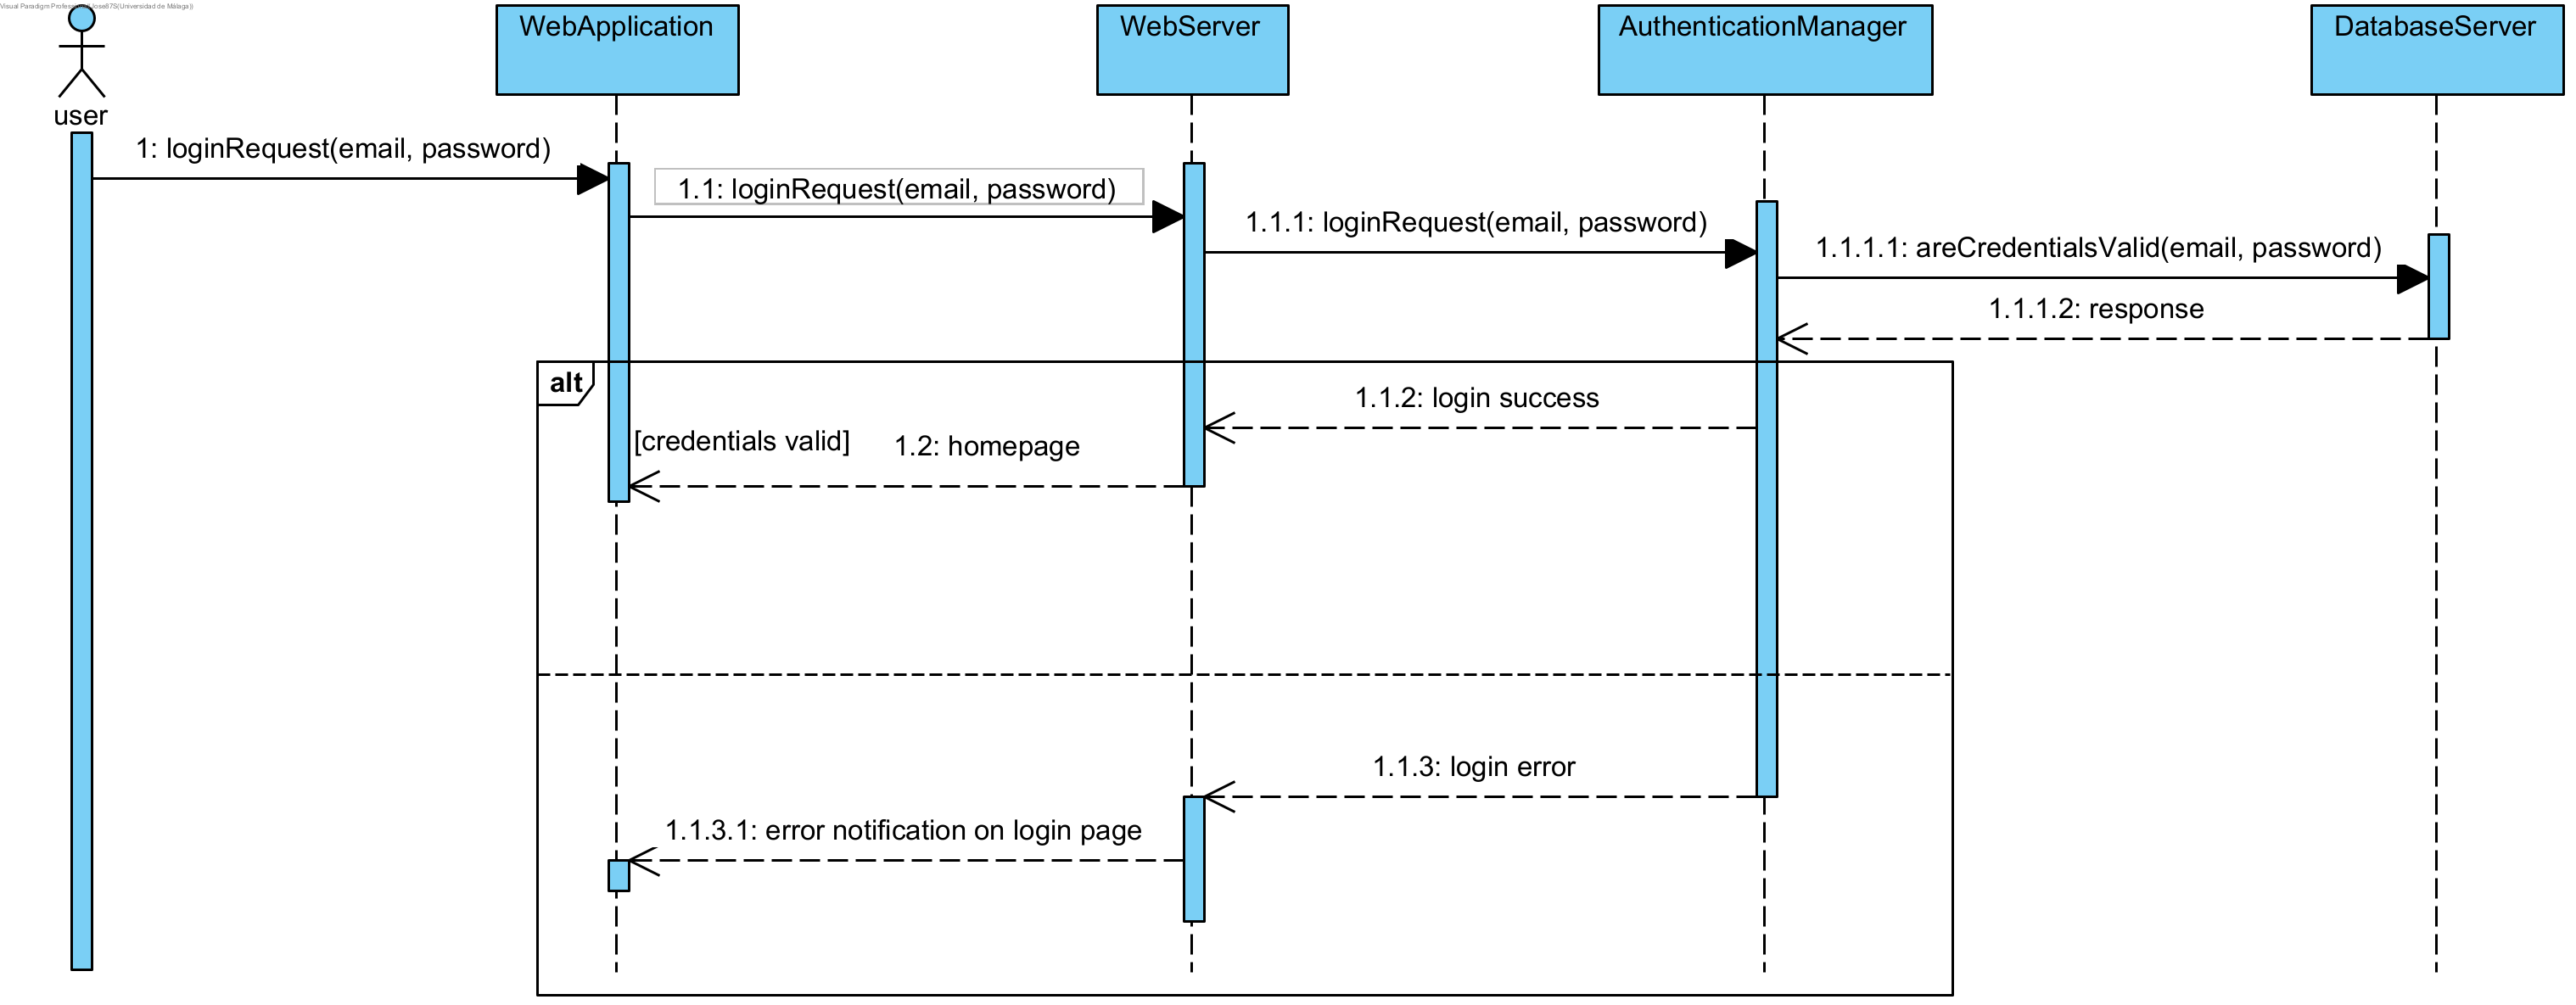
\includegraphics[width=1\textwidth]{images/UseCaseSequenceDiagrams/UC1}
    \caption{Use Case 1}
    \label{fig:UC1}
\end{figure}

\subsubsection*{UC2 - Retrieve Password}

\begin{figure}[H]
    \centering
    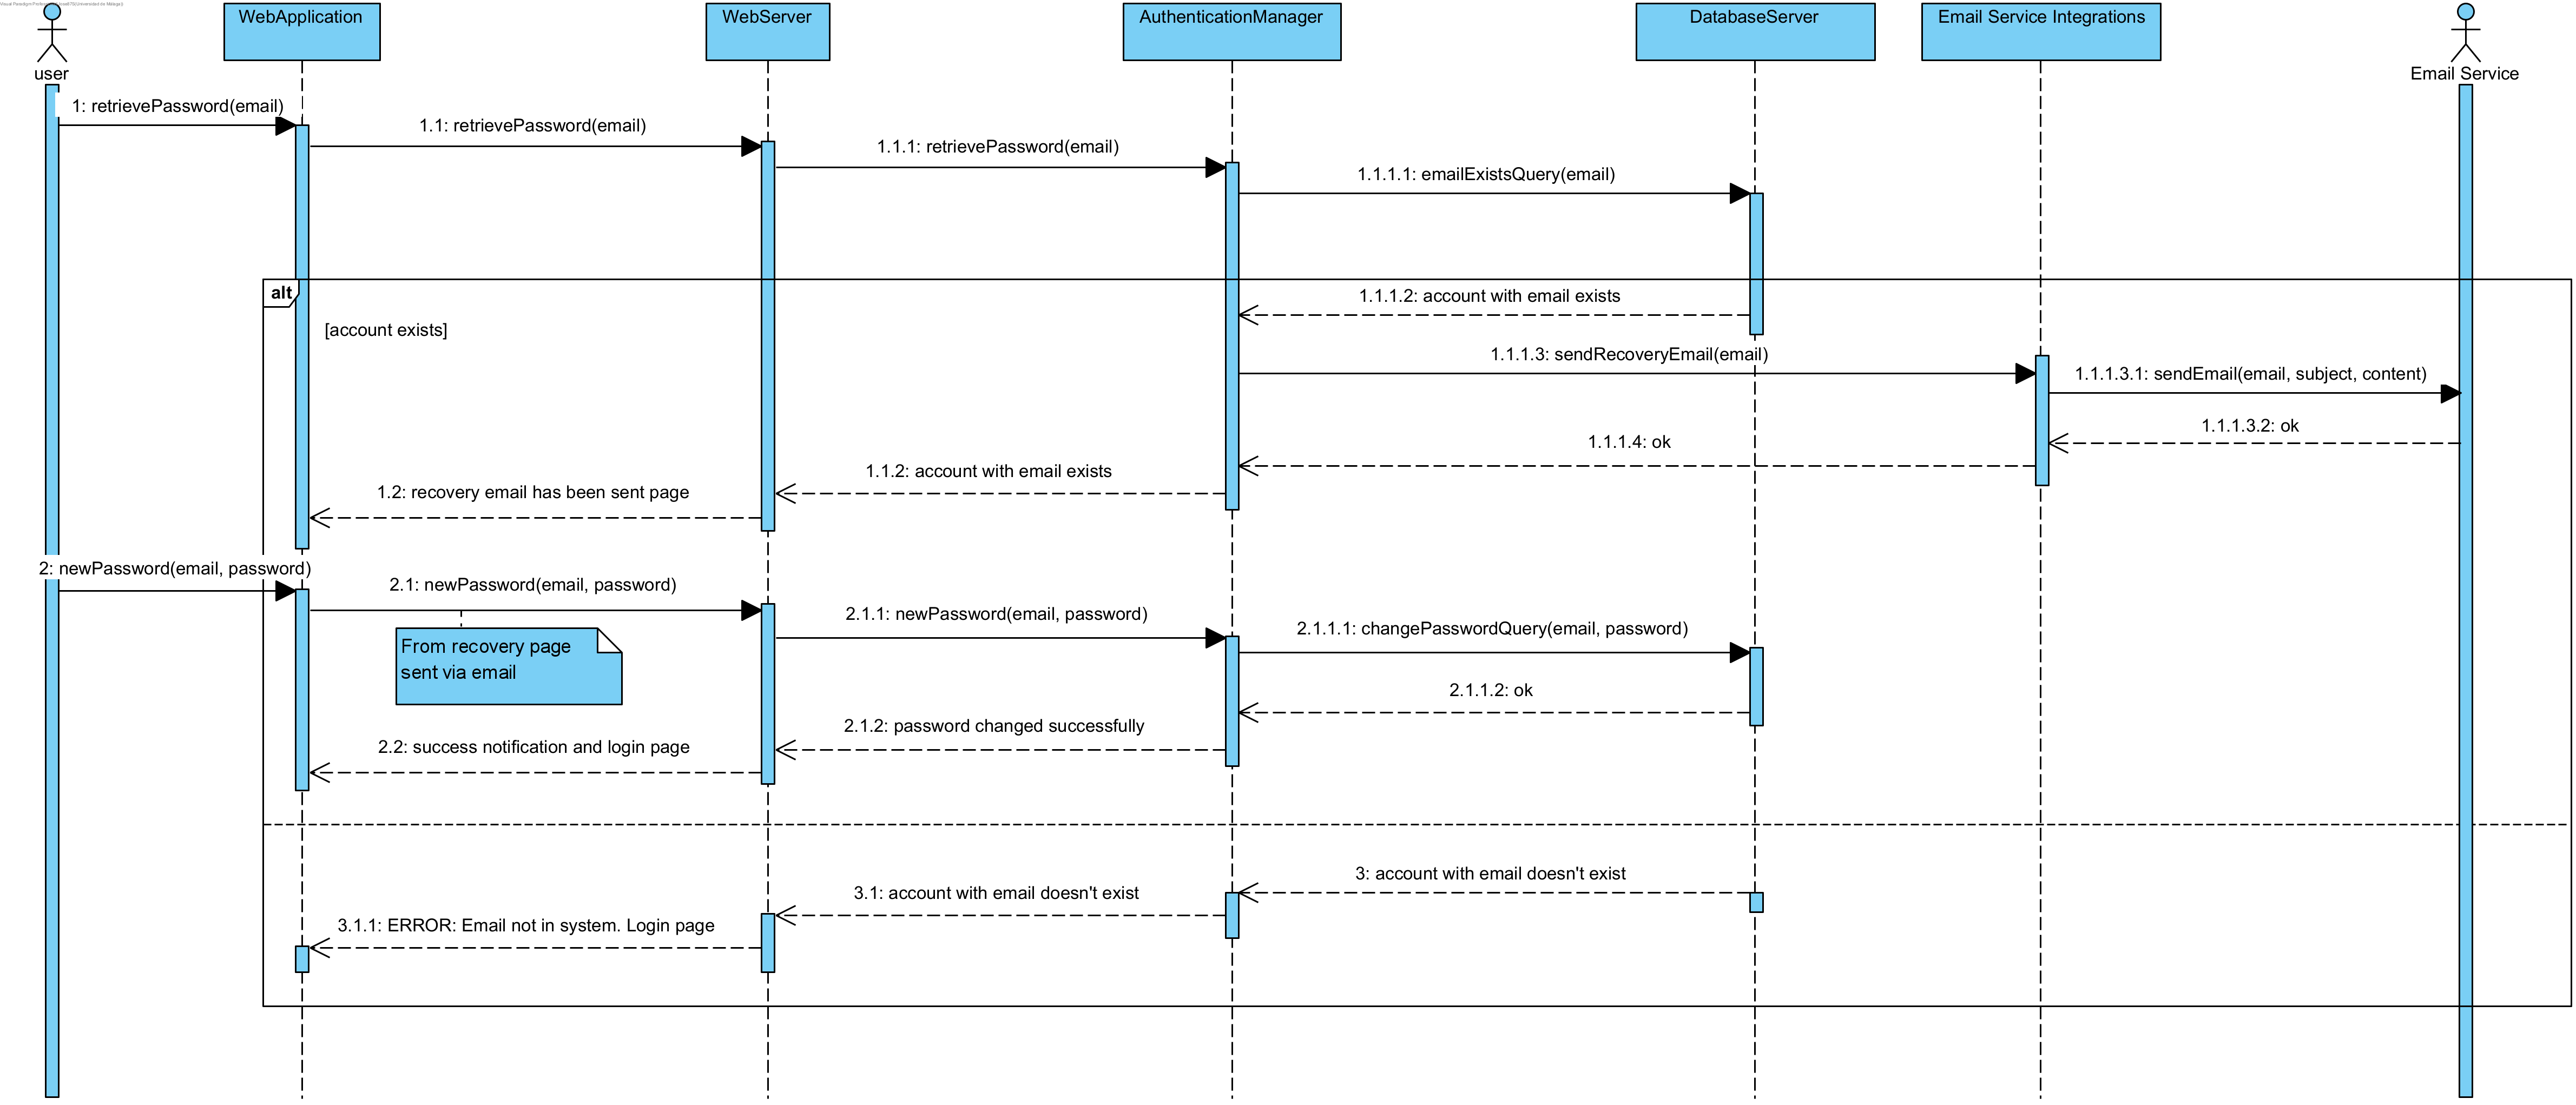
\includegraphics[width=1\textwidth]{images/UseCaseSequenceDiagrams/UC2}
    \caption{Use Case 2}
    \label{fig:UC2}
\end{figure}

\subsubsection*{UC3 - Register}

\begin{figure}[H]
    \centering
    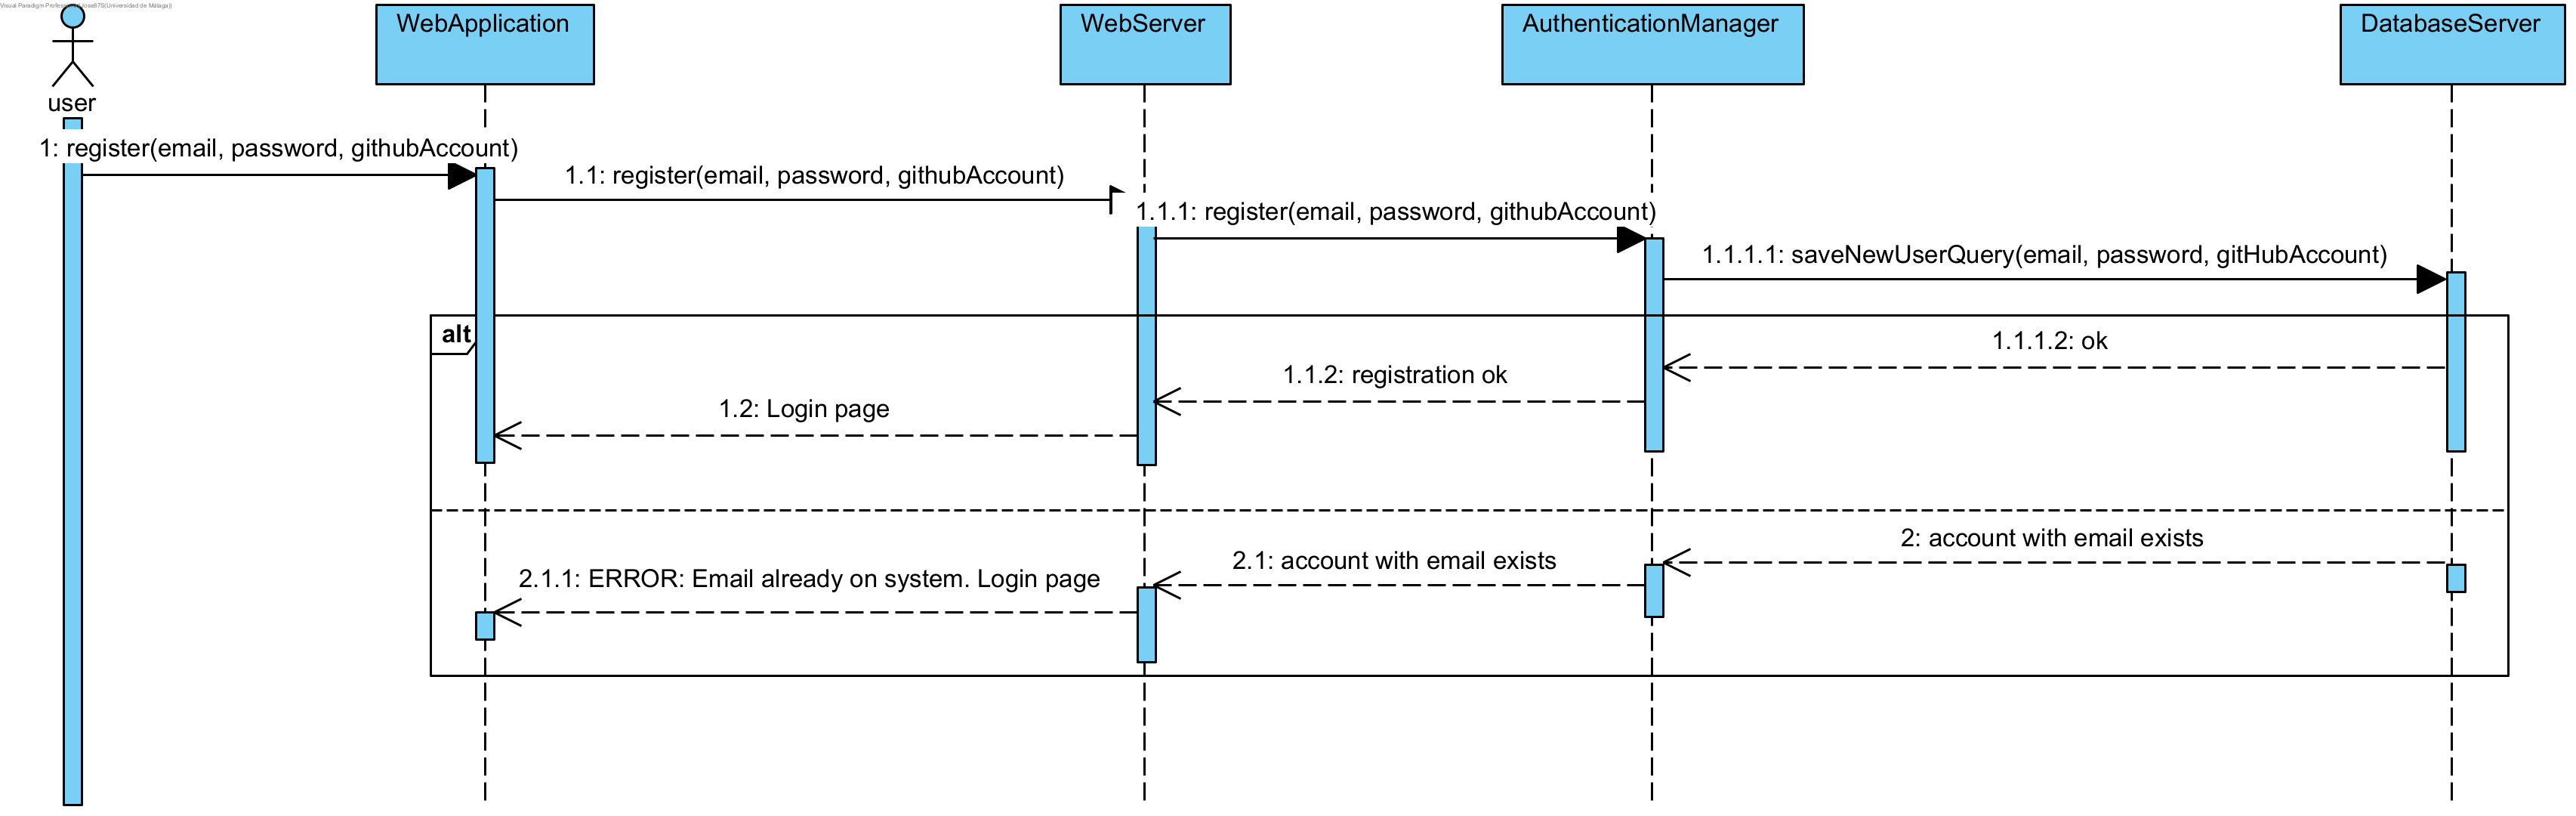
\includegraphics[width=1\textwidth]{images/UseCaseSequenceDiagrams/UC3}
    \caption{Use Case 3}
    \label{fig:UC3}
\end{figure}

\subsubsection*{UC4 - Educator Creates Tournament}

\begin{figure}[H]
    \centering
    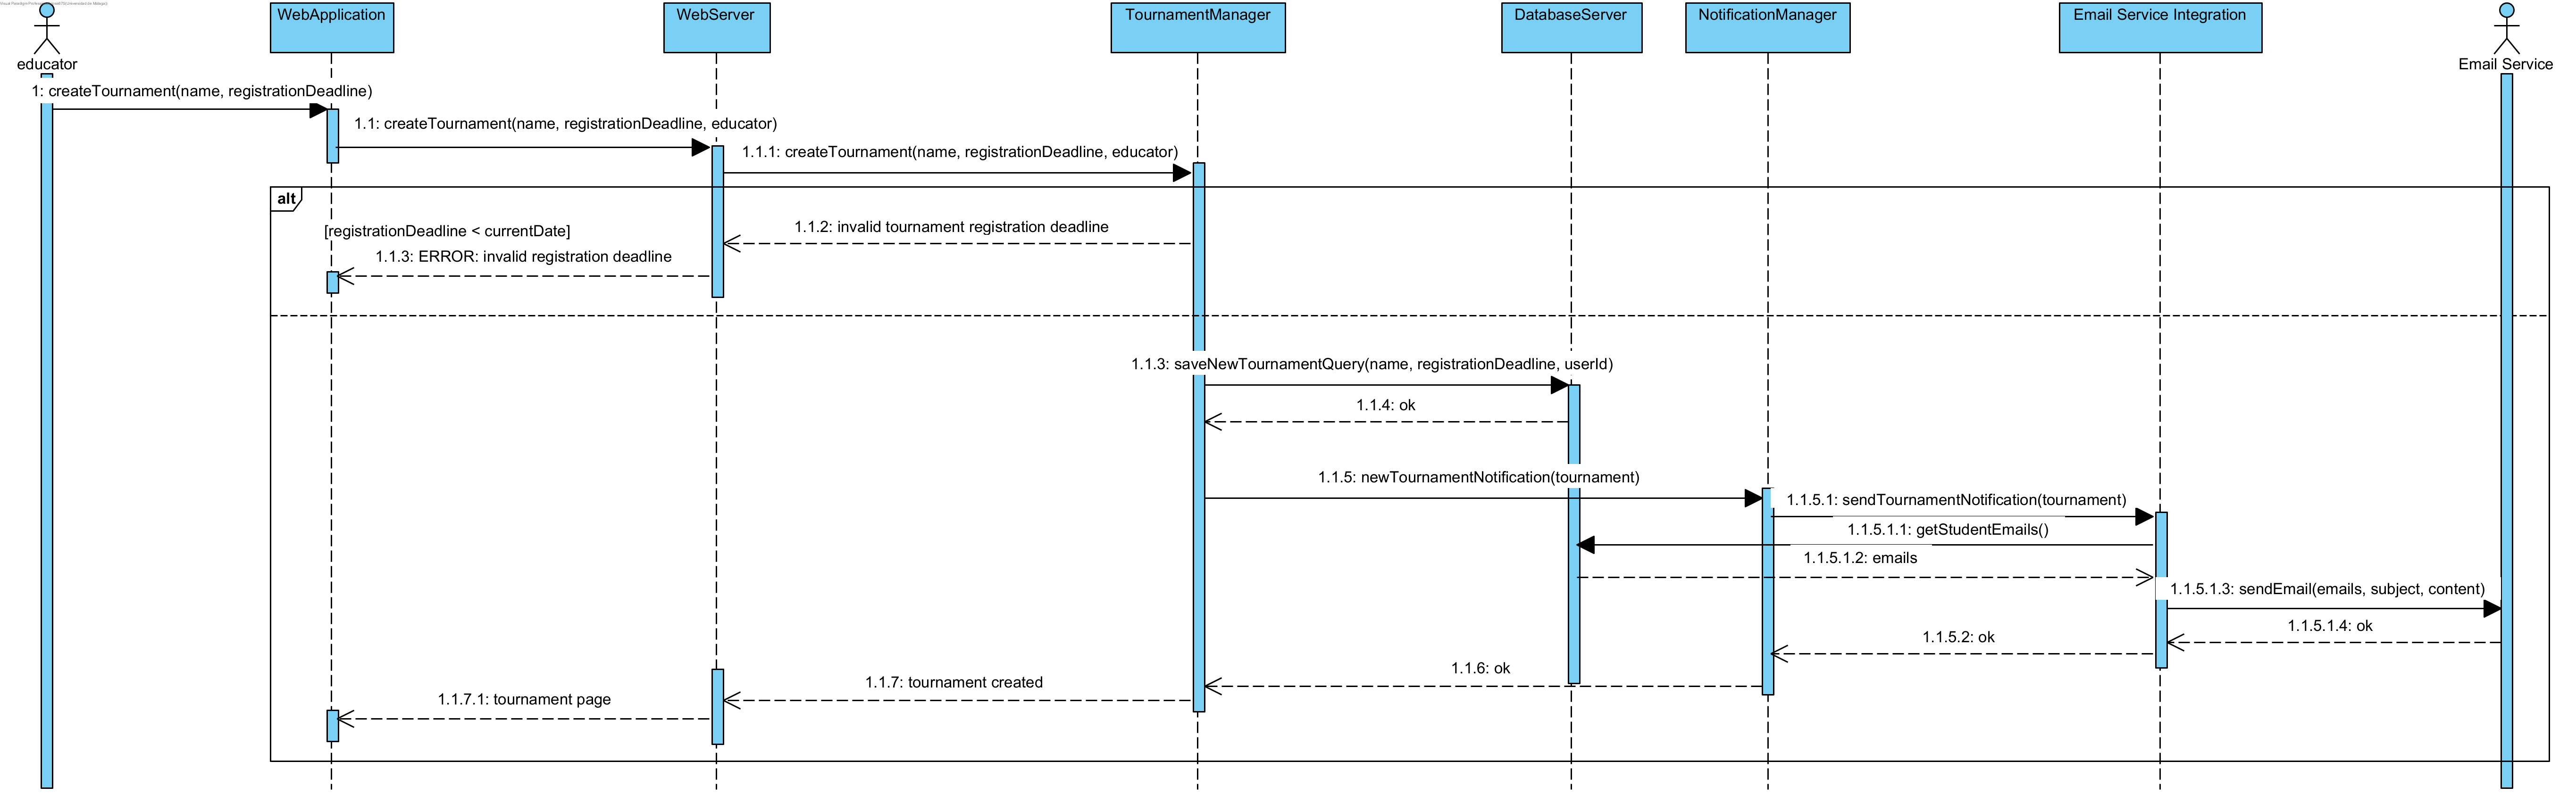
\includegraphics[width=1\textwidth]{images/UseCaseSequenceDiagrams/UC4}
    \caption{Use Case 4}
    \label{fig:UC4}
\end{figure}

\subsubsection*{UC5 - Educator invites other educator to tournament}

\begin{figure}[H]
    \centering
    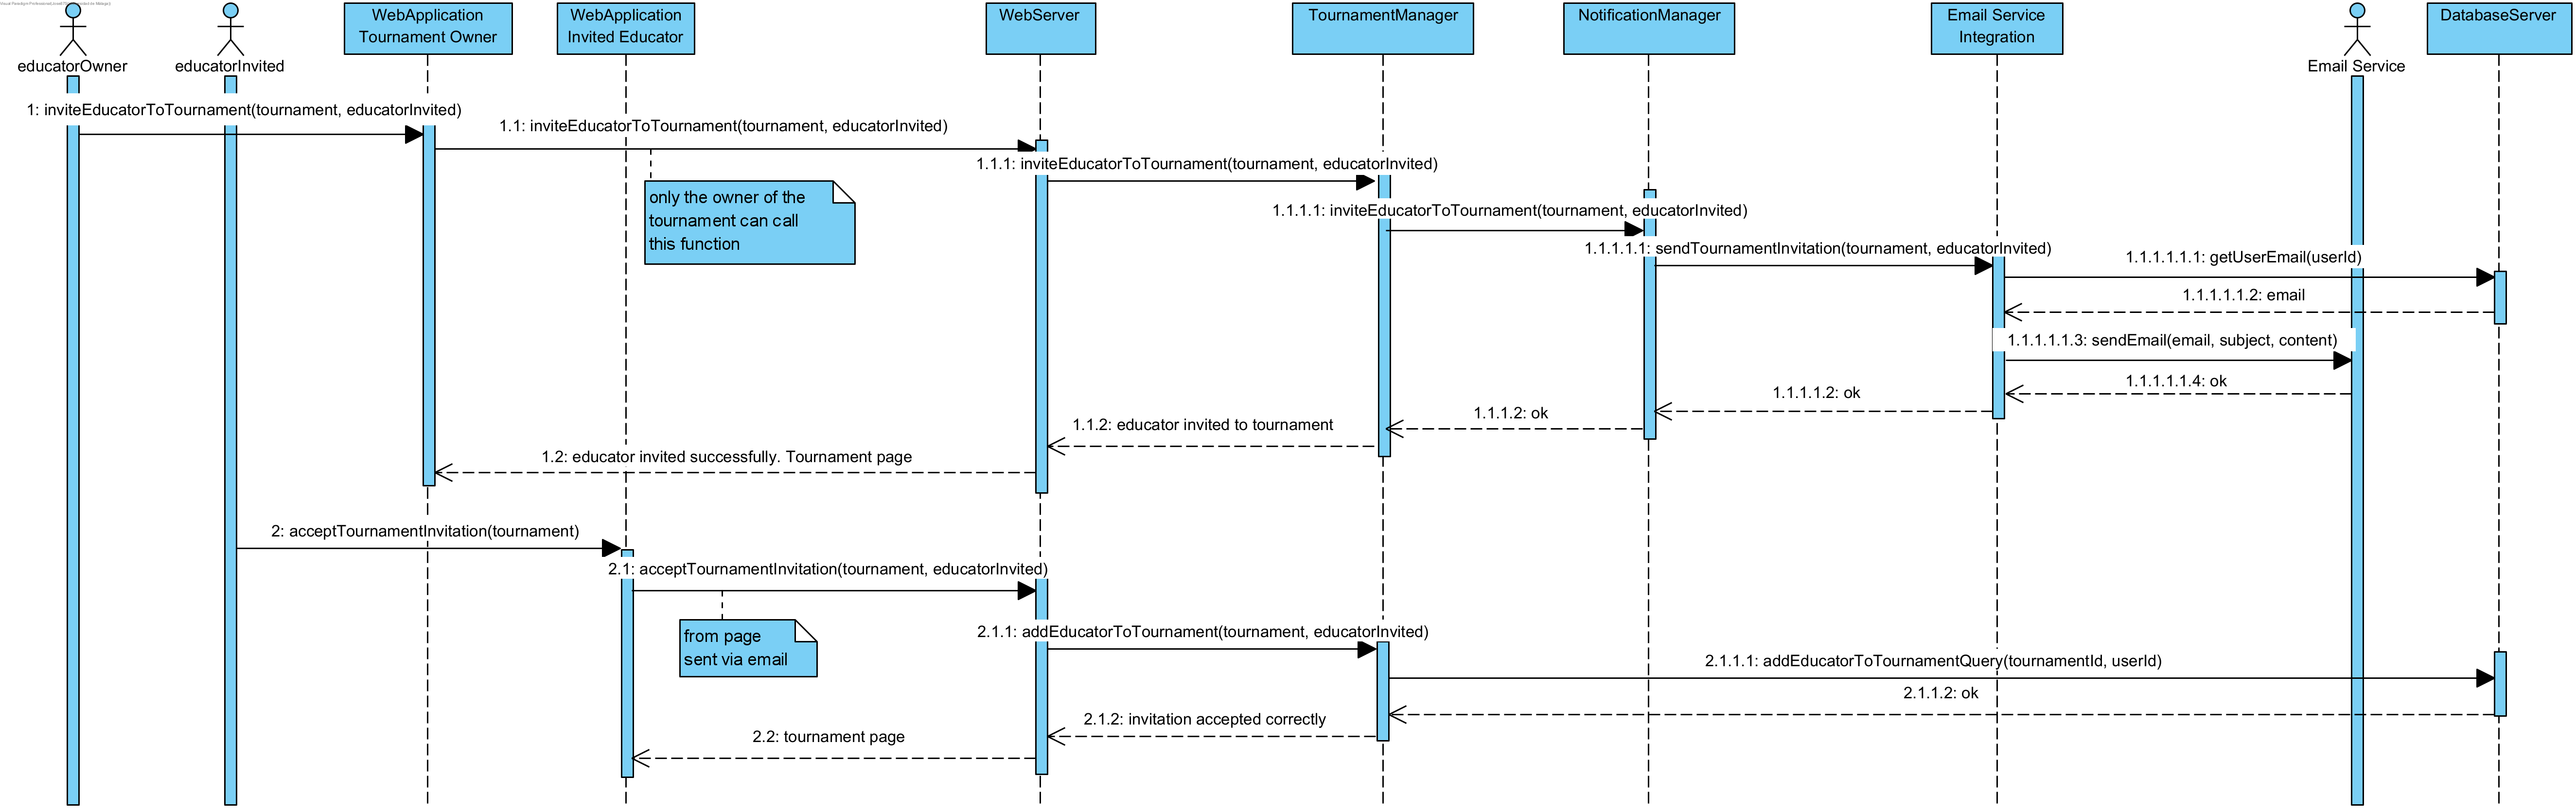
\includegraphics[width=1\textwidth]{images/UseCaseSequenceDiagrams/UC5}
    \caption{Use Case 5}
    \label{fig:UC5}
\end{figure}

\subsubsection*{UC6 - Educator creates battle}

\begin{figure}[H]
    \centering
    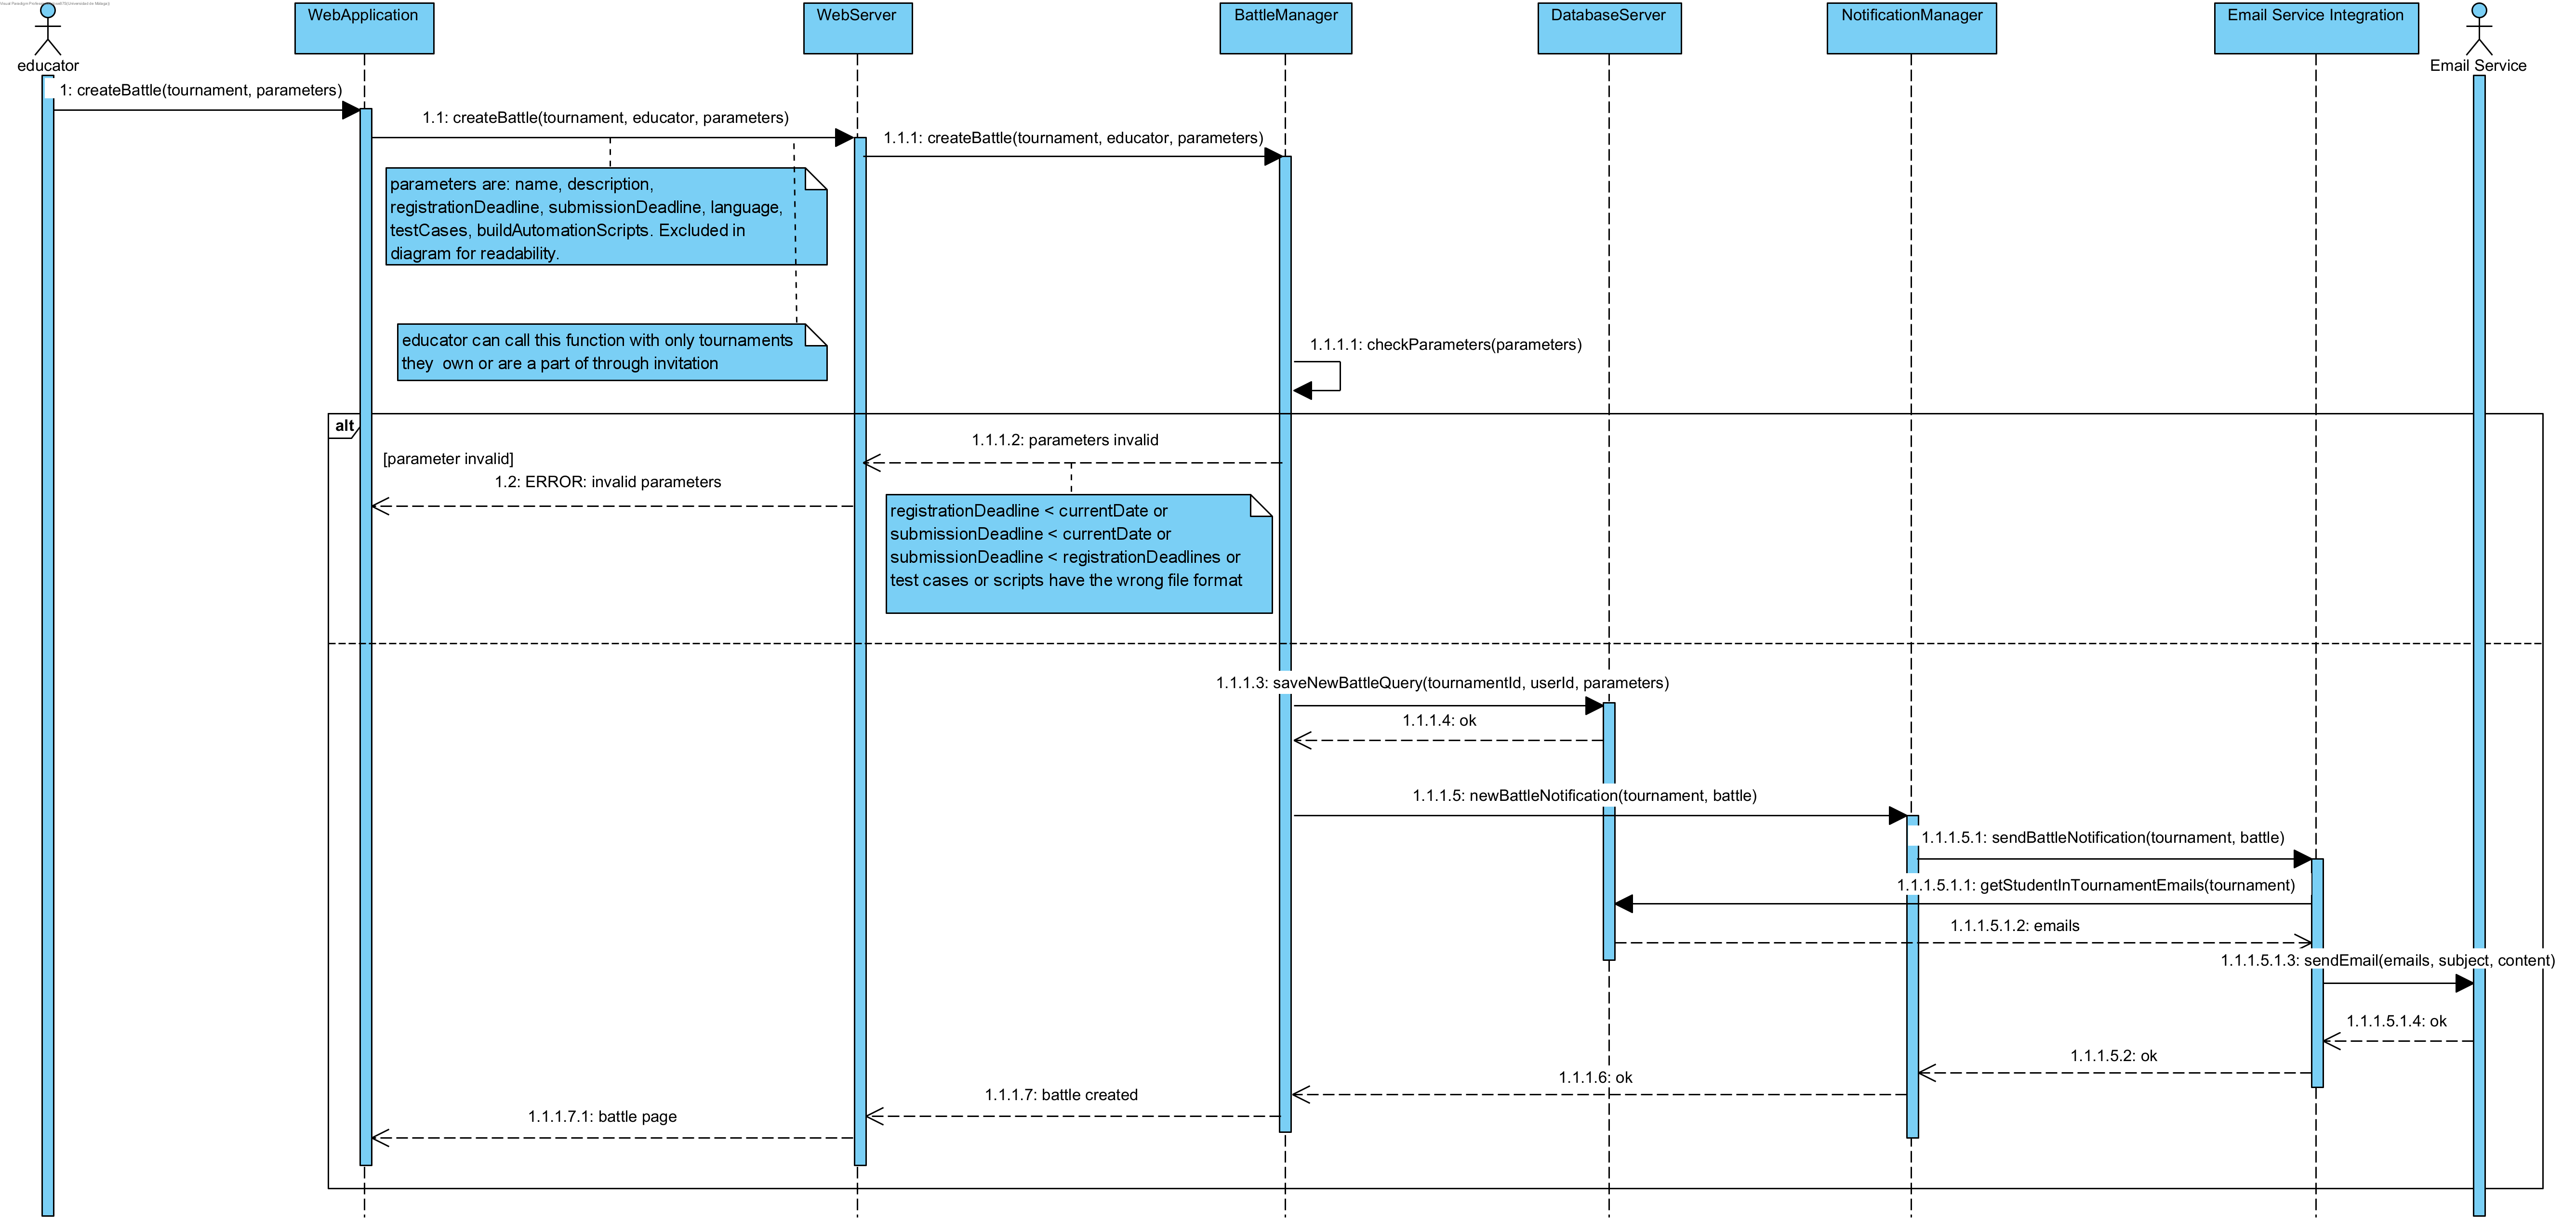
\includegraphics[width=1\textwidth]{images/UseCaseSequenceDiagrams/UC6}
    \caption{Use Case 6}
    \label{fig:UC6}
\end{figure}

\subsubsection*{UC7 - Tournament Registration}

\begin{figure}[H]
    \centering
    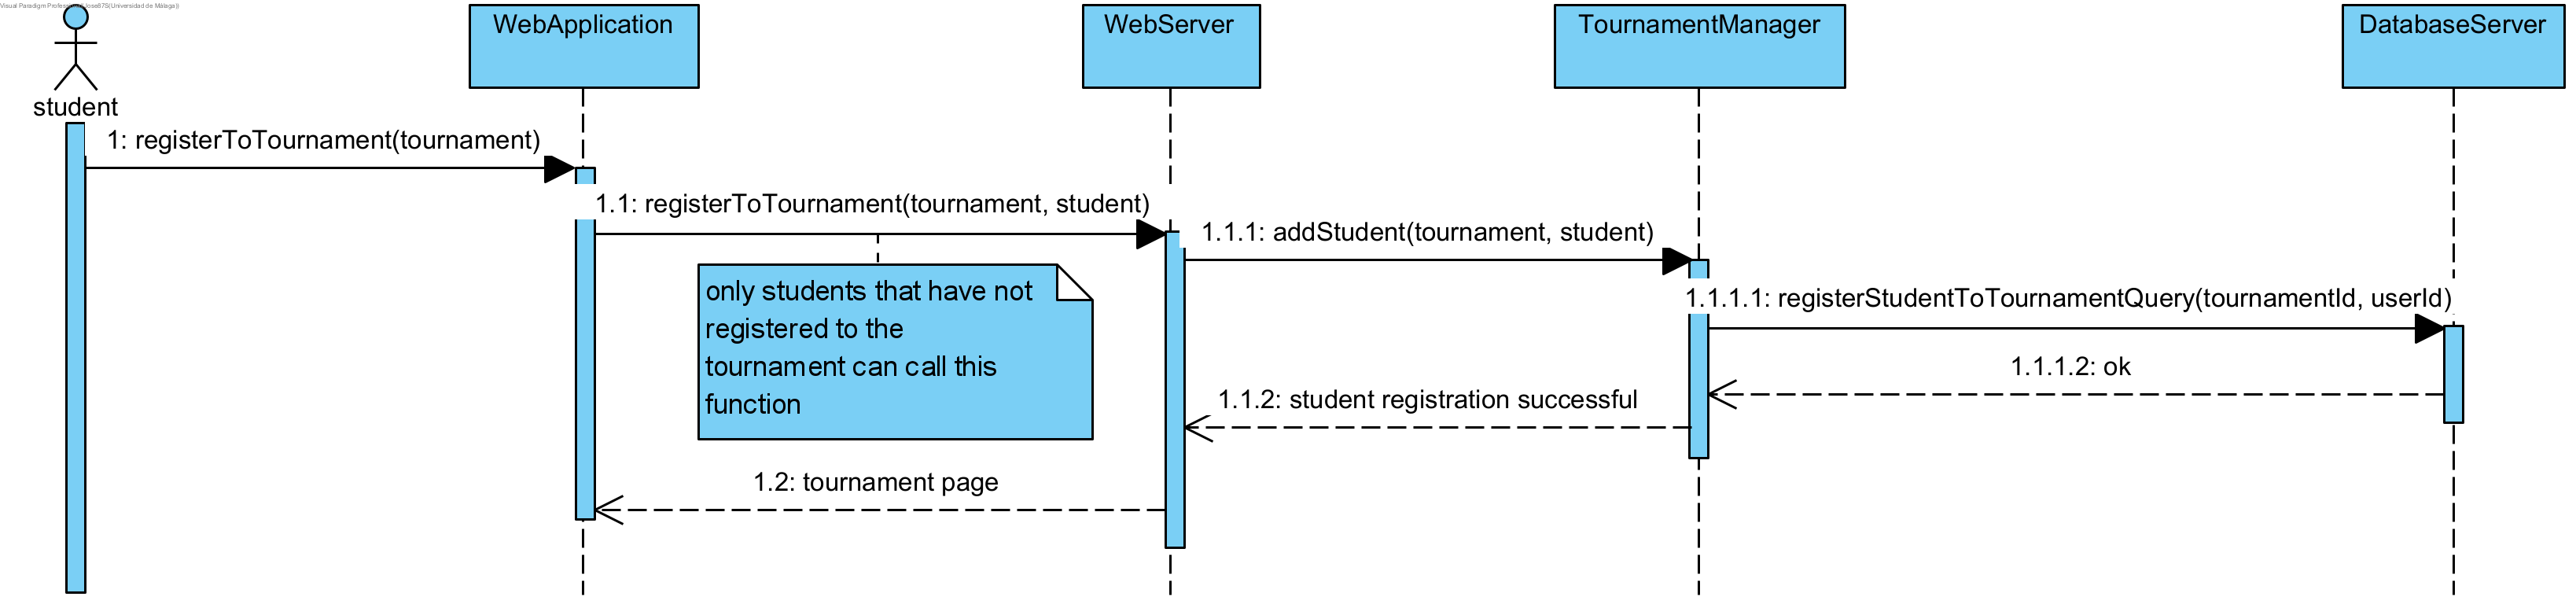
\includegraphics[width=1\textwidth]{images/UseCaseSequenceDiagrams/UC7}
    \caption{Use Case 7}
    \label{fig:UC7}
\end{figure}

\subsubsection*{UC8 - Tournament Unregistration}

\begin{figure}[H]
    \centering
    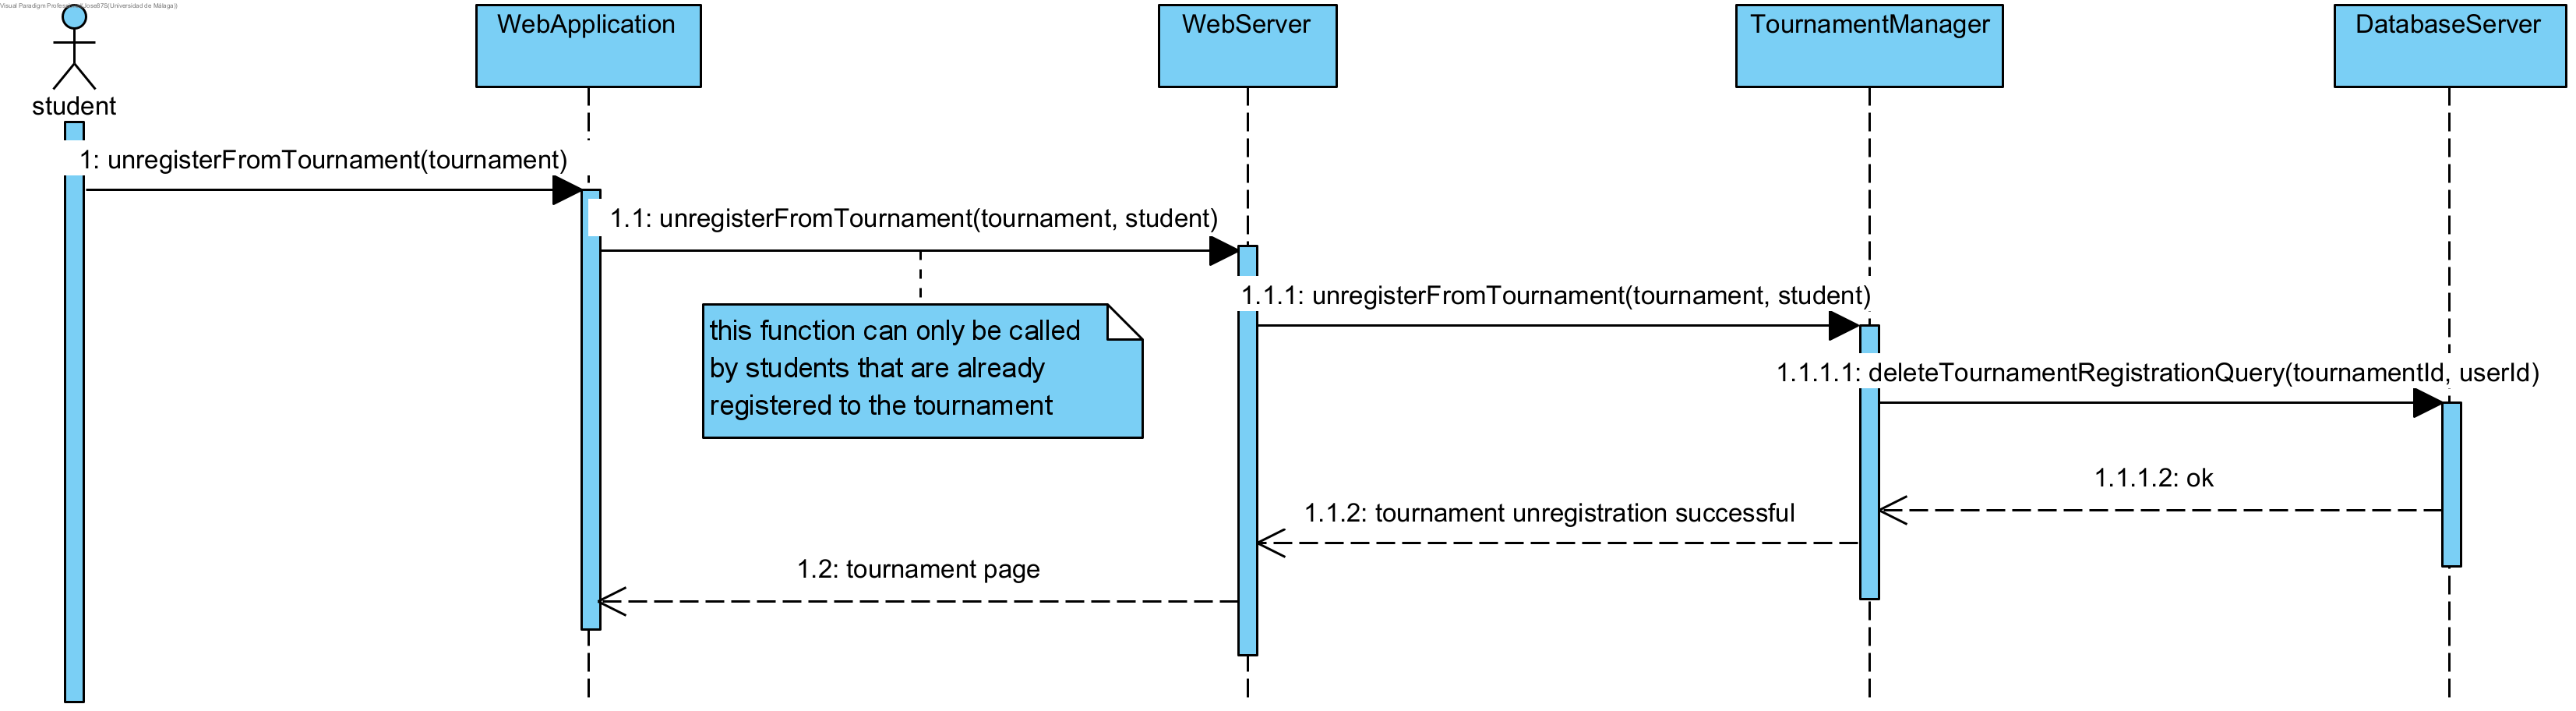
\includegraphics[width=1\textwidth]{images/UseCaseSequenceDiagrams/UC8}
    \caption{Use Case 8}
    \label{fig:UC8}
\end{figure}

\subsubsection*{UC9 - Battle Registration}

\begin{figure}[H]
    \centering
    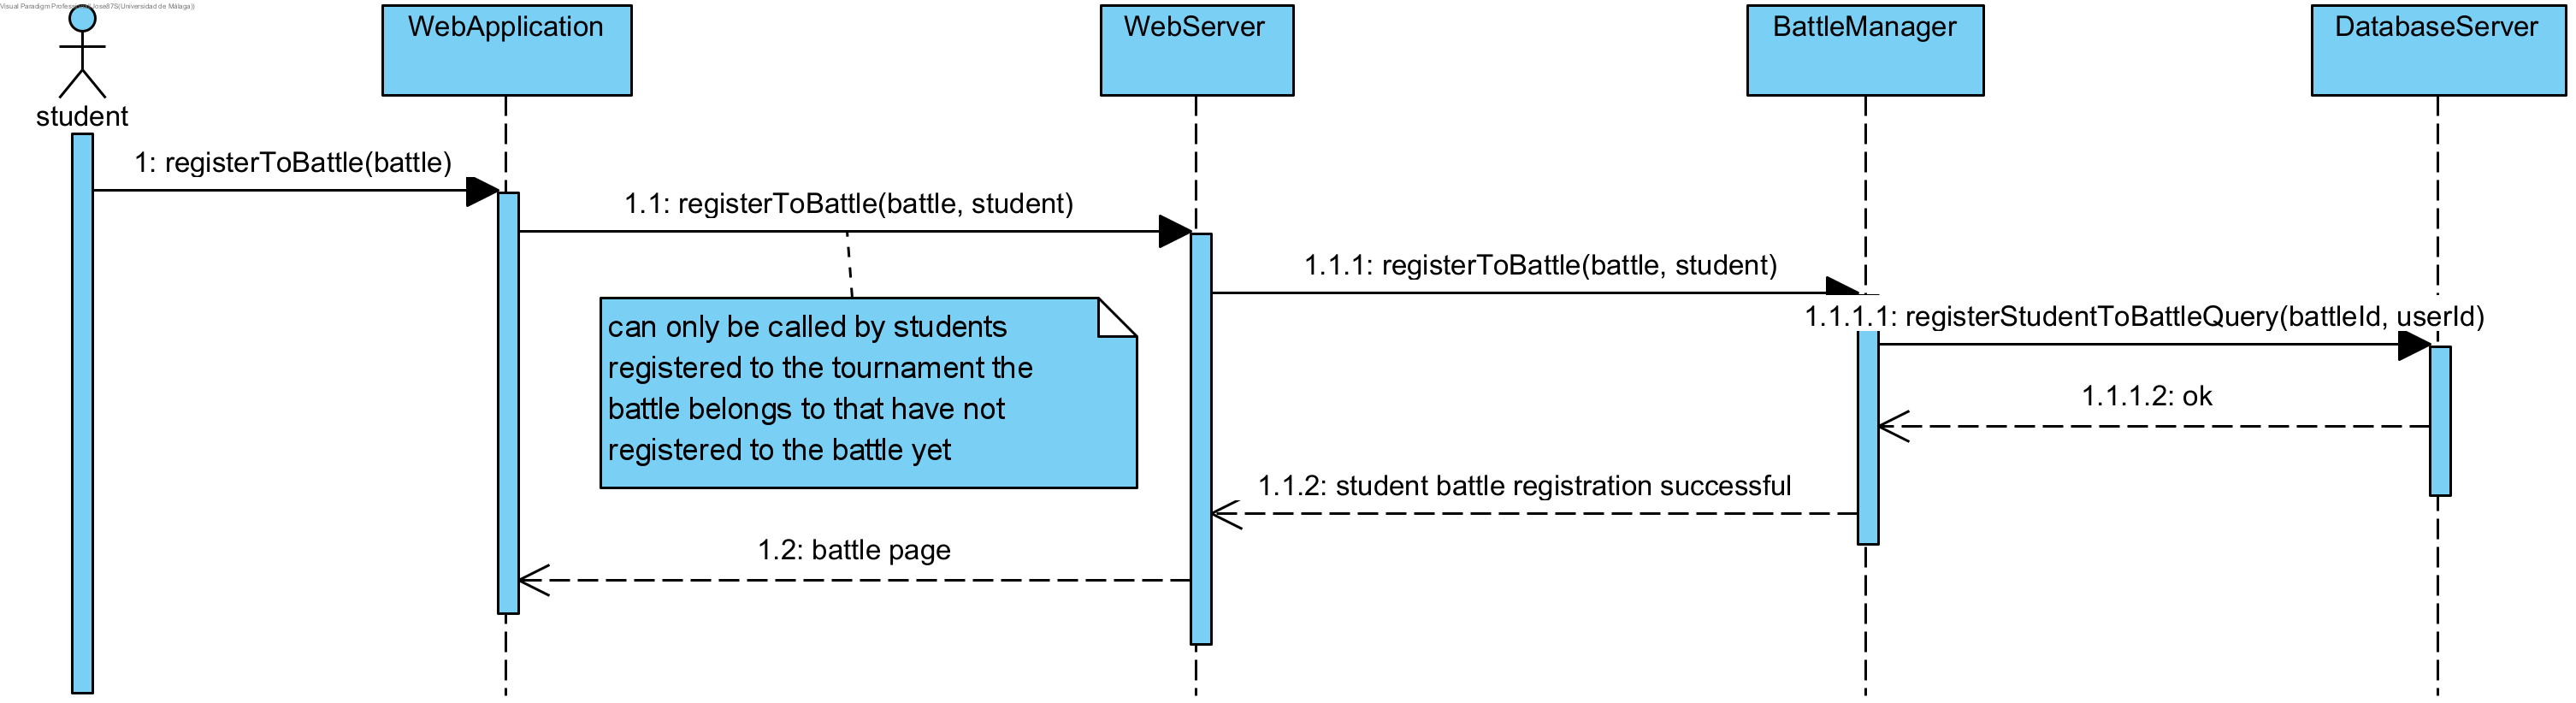
\includegraphics[width=1\textwidth]{images/UseCaseSequenceDiagrams/UC9}
    \caption{Use Case 9}
    \label{fig:UC9}
\end{figure}

\subsubsection*{UC10 - Student joins battle via invite}

\begin{figure}[H]
    \centering
    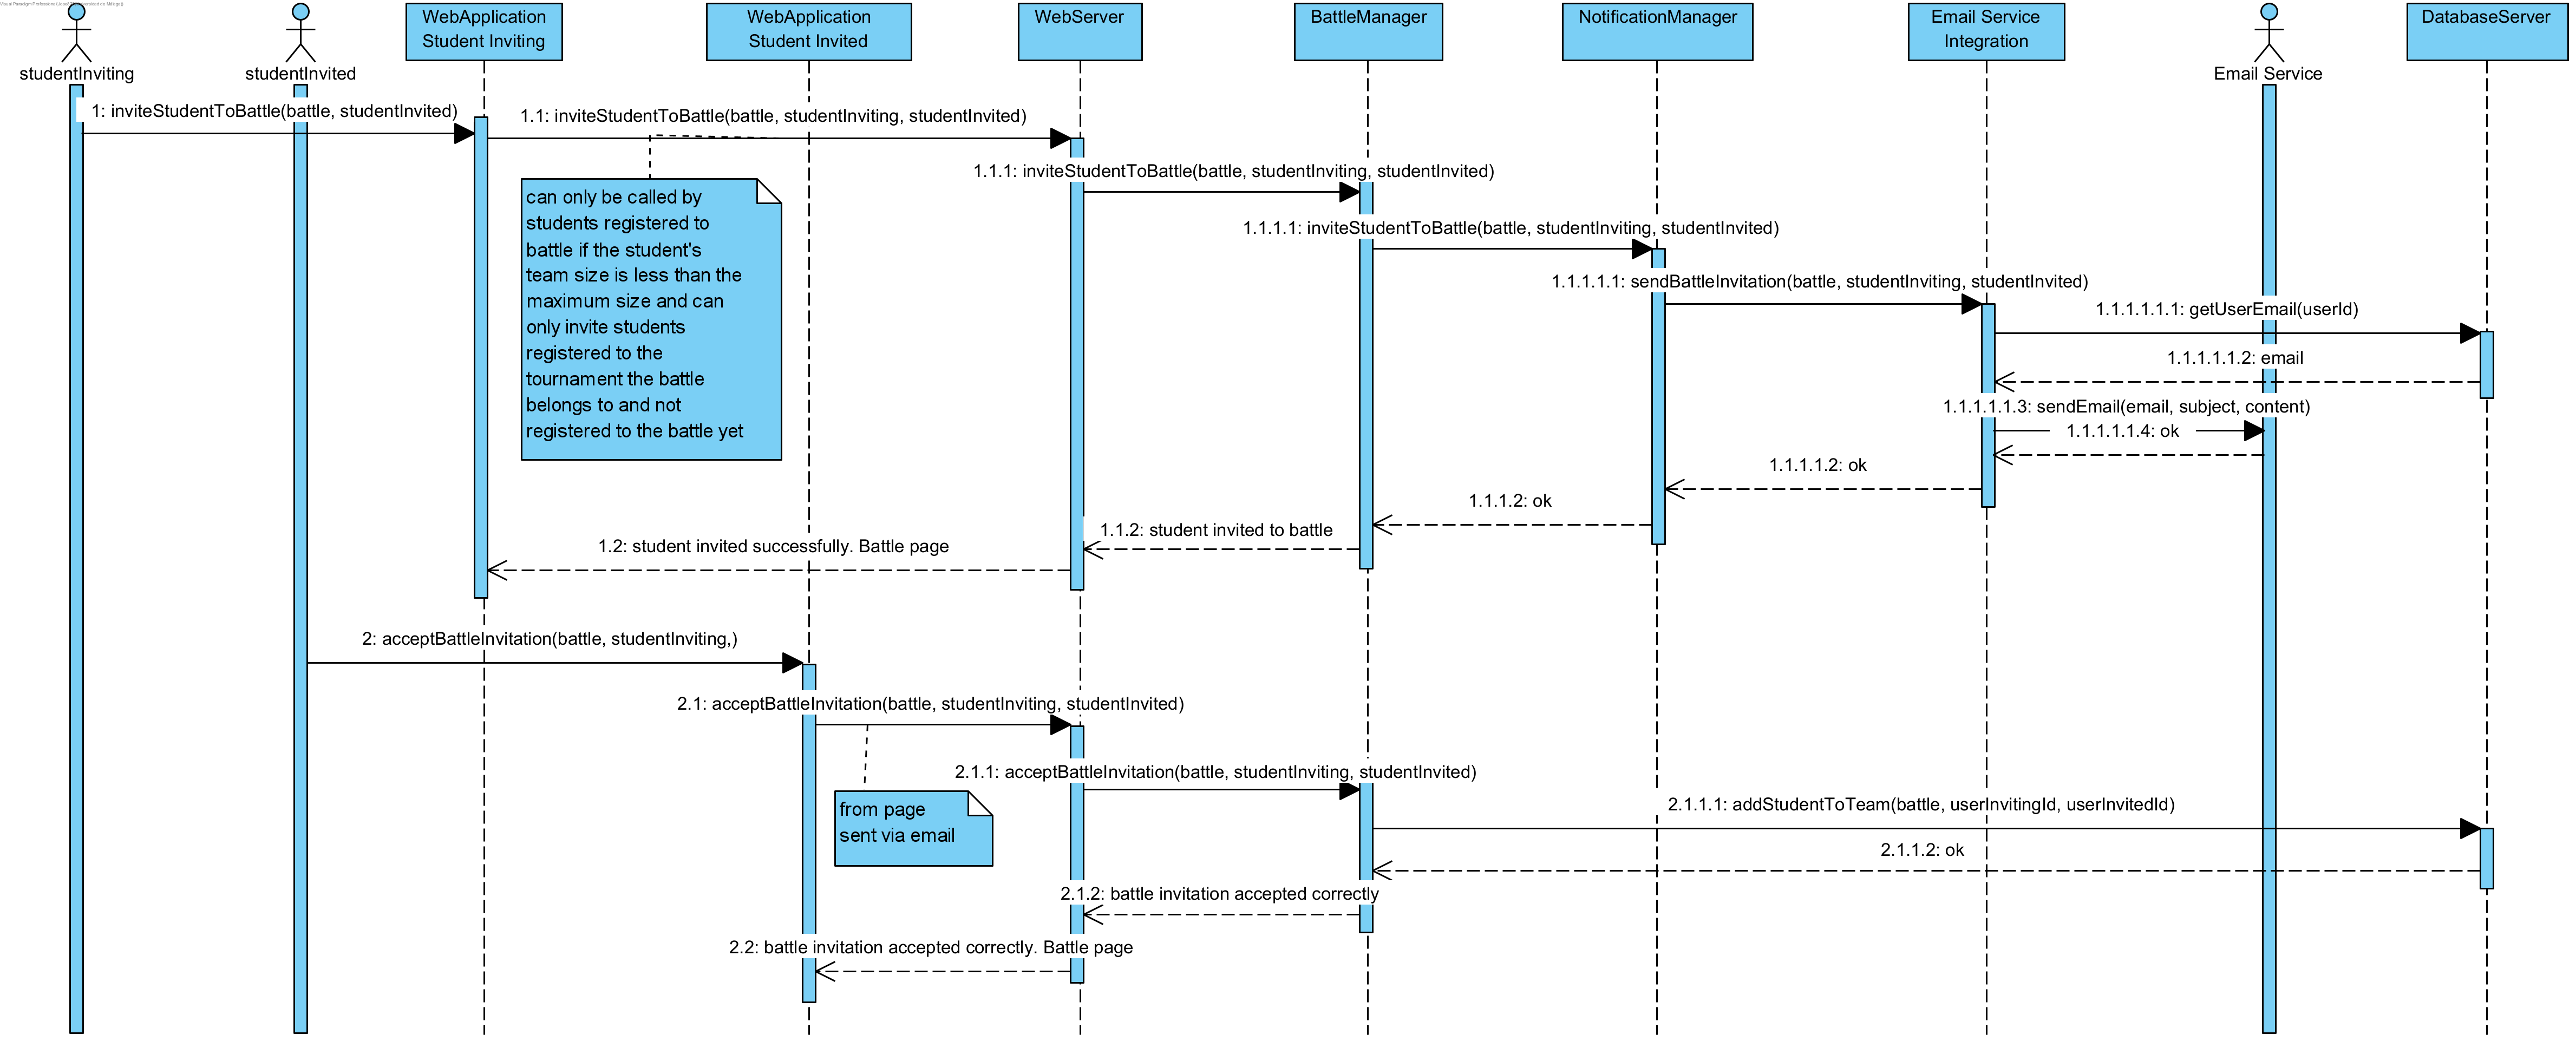
\includegraphics[width=1\textwidth]{images/UseCaseSequenceDiagrams/UC10}
    \caption{Use Case 10}
    \label{fig:UC10}
\end{figure}

\subsubsection*{UC11 - Battle Unregistration}

\begin{figure}[H]
    \centering
    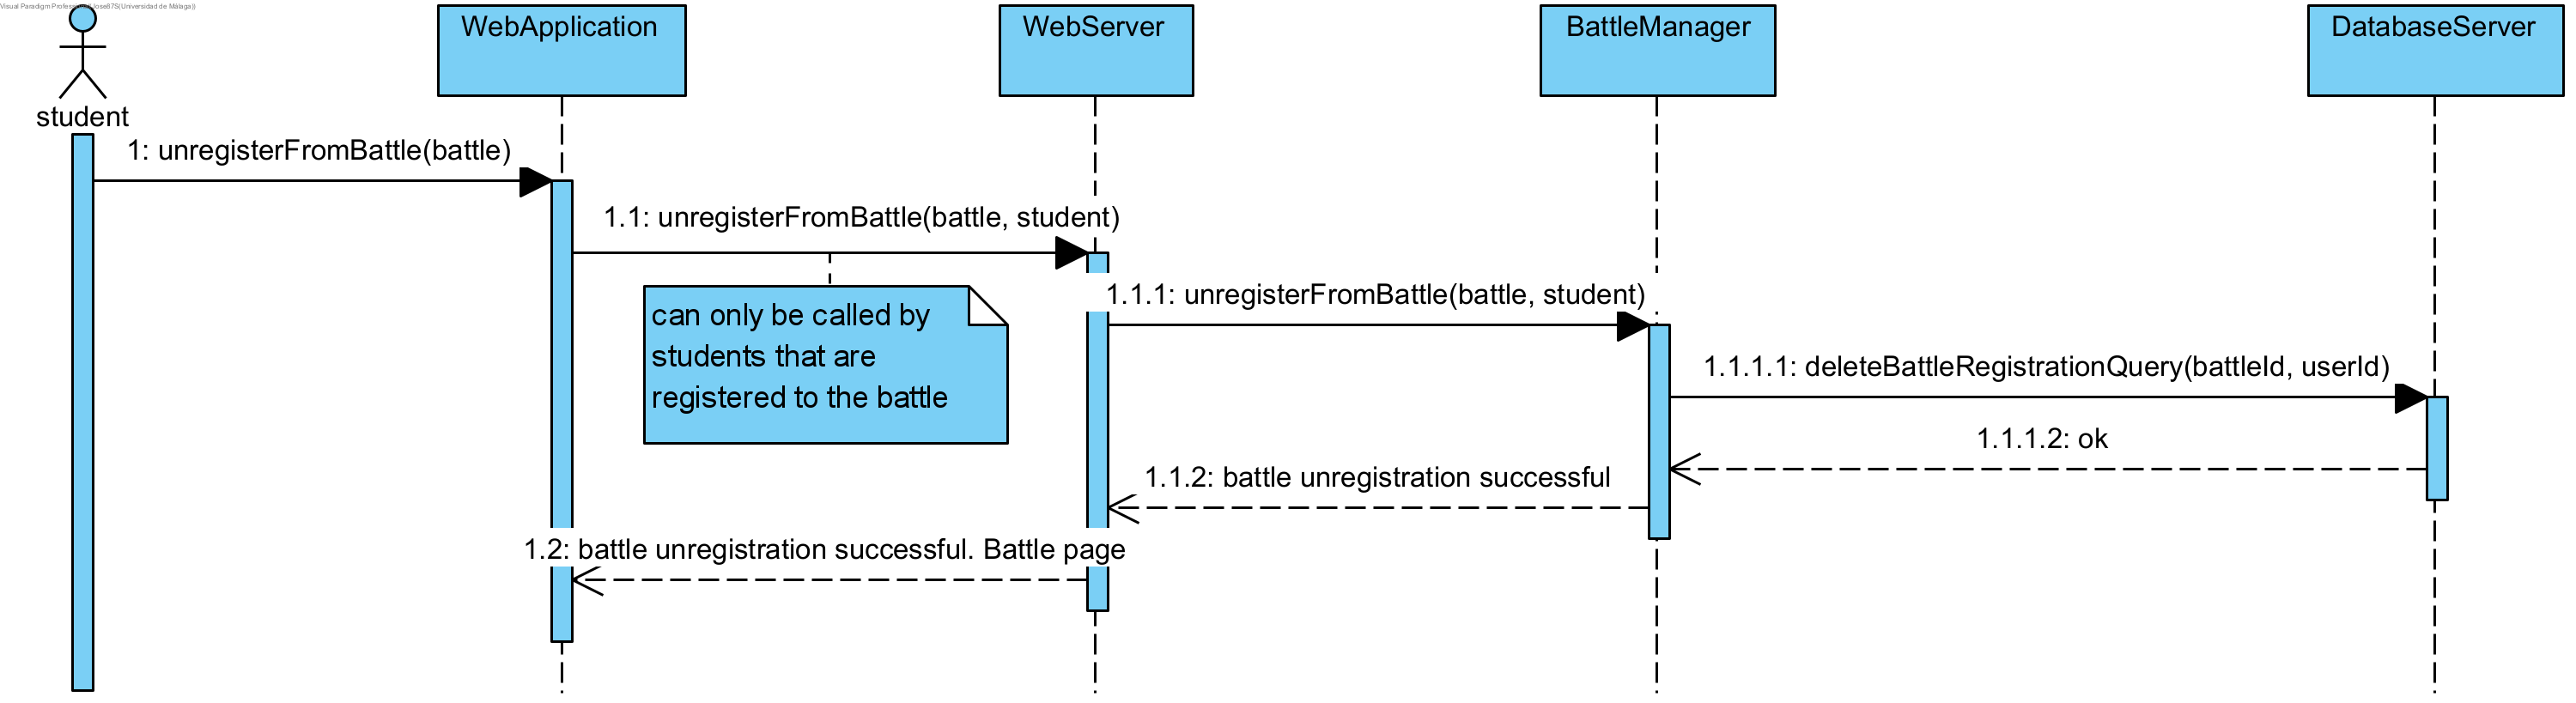
\includegraphics[width=1\textwidth]{images/UseCaseSequenceDiagrams/UC11}
    \caption{Use Case 11}
    \label{fig:UC11}
\end{figure}

\subsubsection*{UC12 - Students makes submission}

\begin{figure}[H]
    \centering
    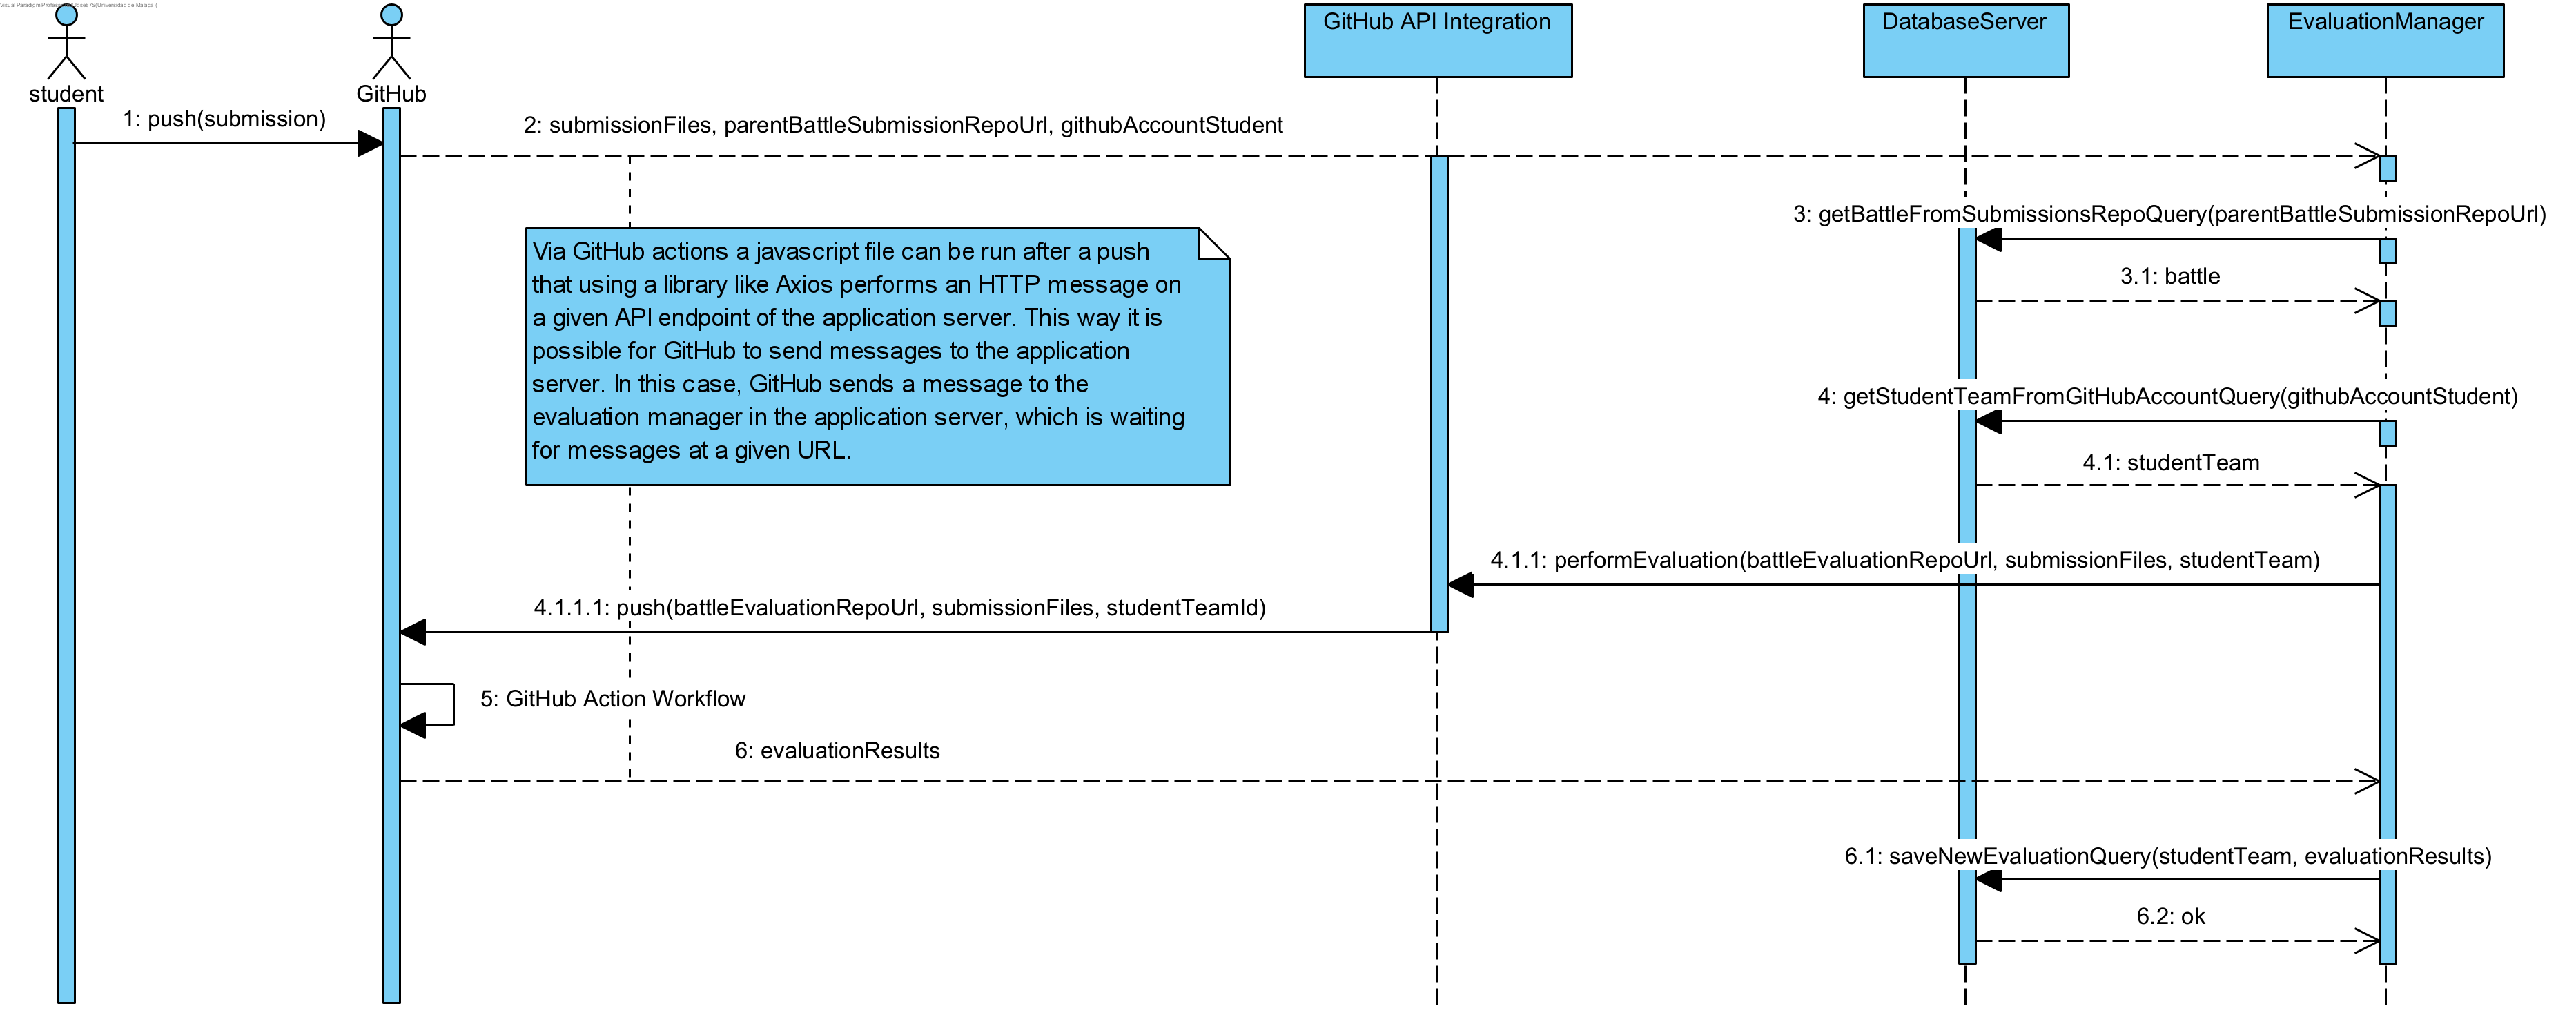
\includegraphics[width=1\textwidth]{images/UseCaseSequenceDiagrams/UC12}
    \caption{Use Case 12}
    \label{fig:UC12}
\end{figure}

\subsubsection*{UC13 - Educator Performs Manual Evaluations and Closes Battle}

\begin{figure}[H]
    \centering
    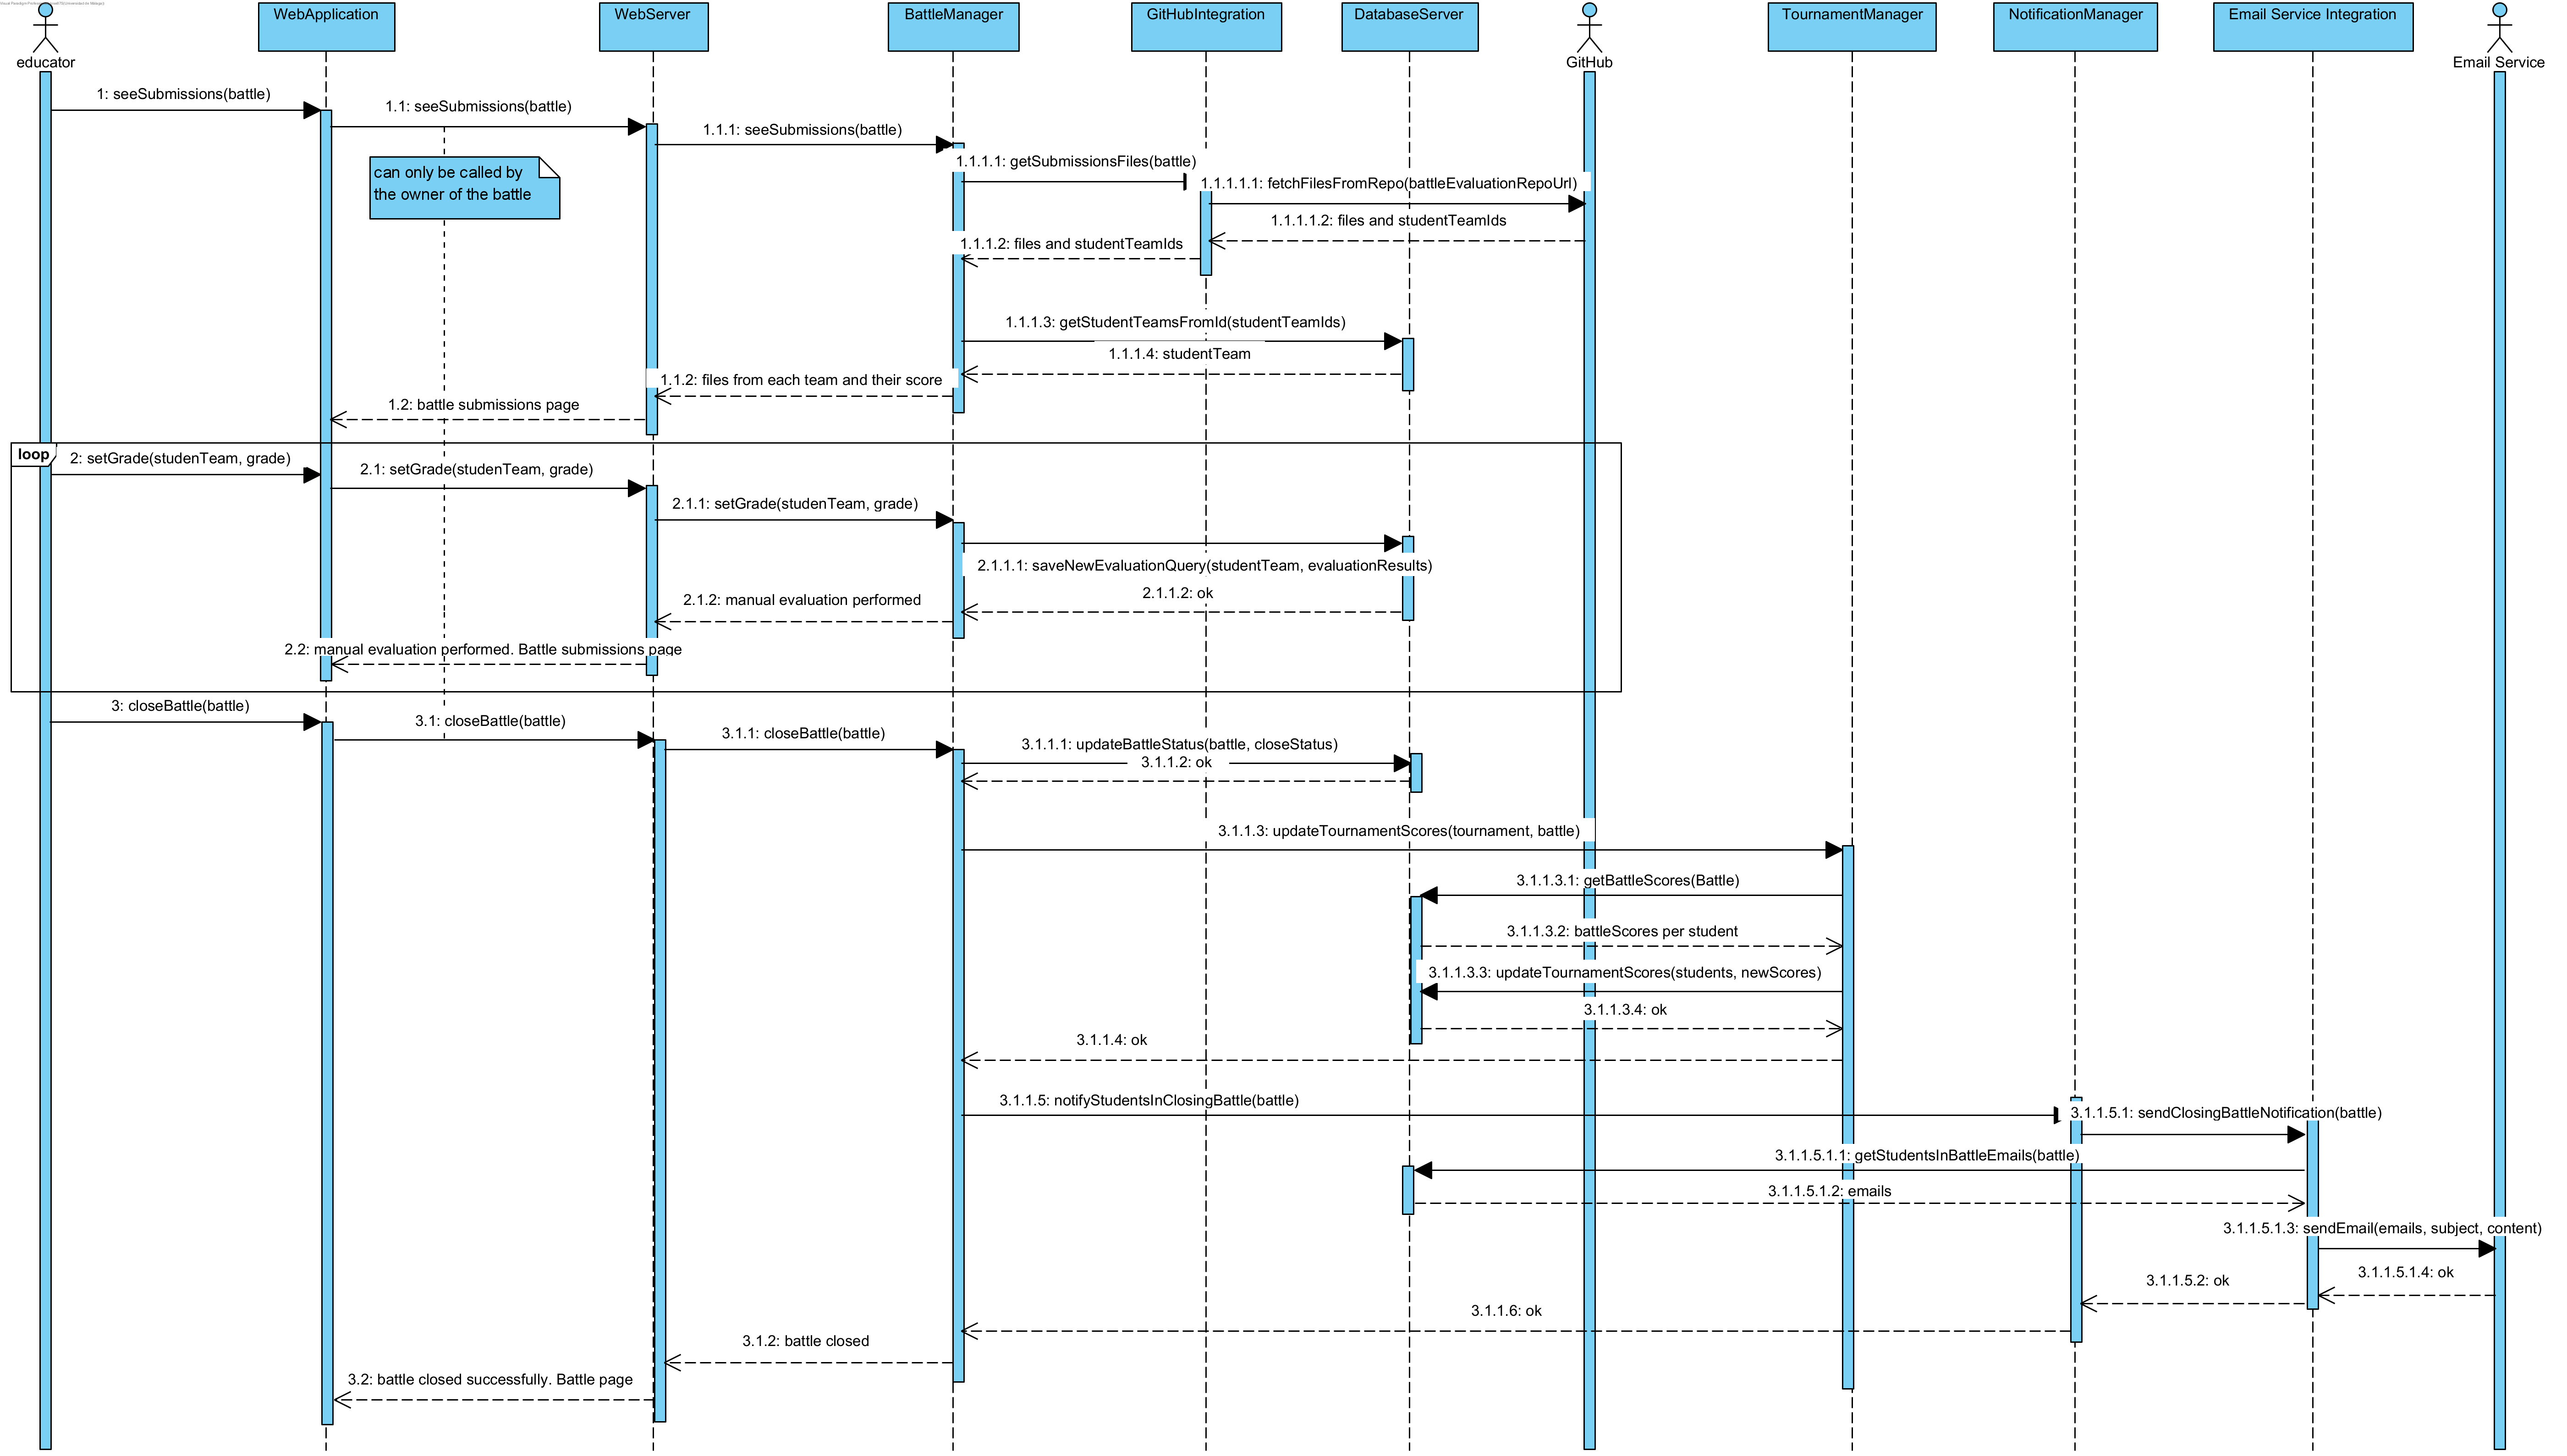
\includegraphics[width=1\textwidth]{images/UseCaseSequenceDiagrams/UC13}
    \caption{Use Case 13}
    \label{fig:UC13}
\end{figure}

\subsubsection*{UC14 - Educator Closes Tournament}

\begin{figure}[H]
    \centering
    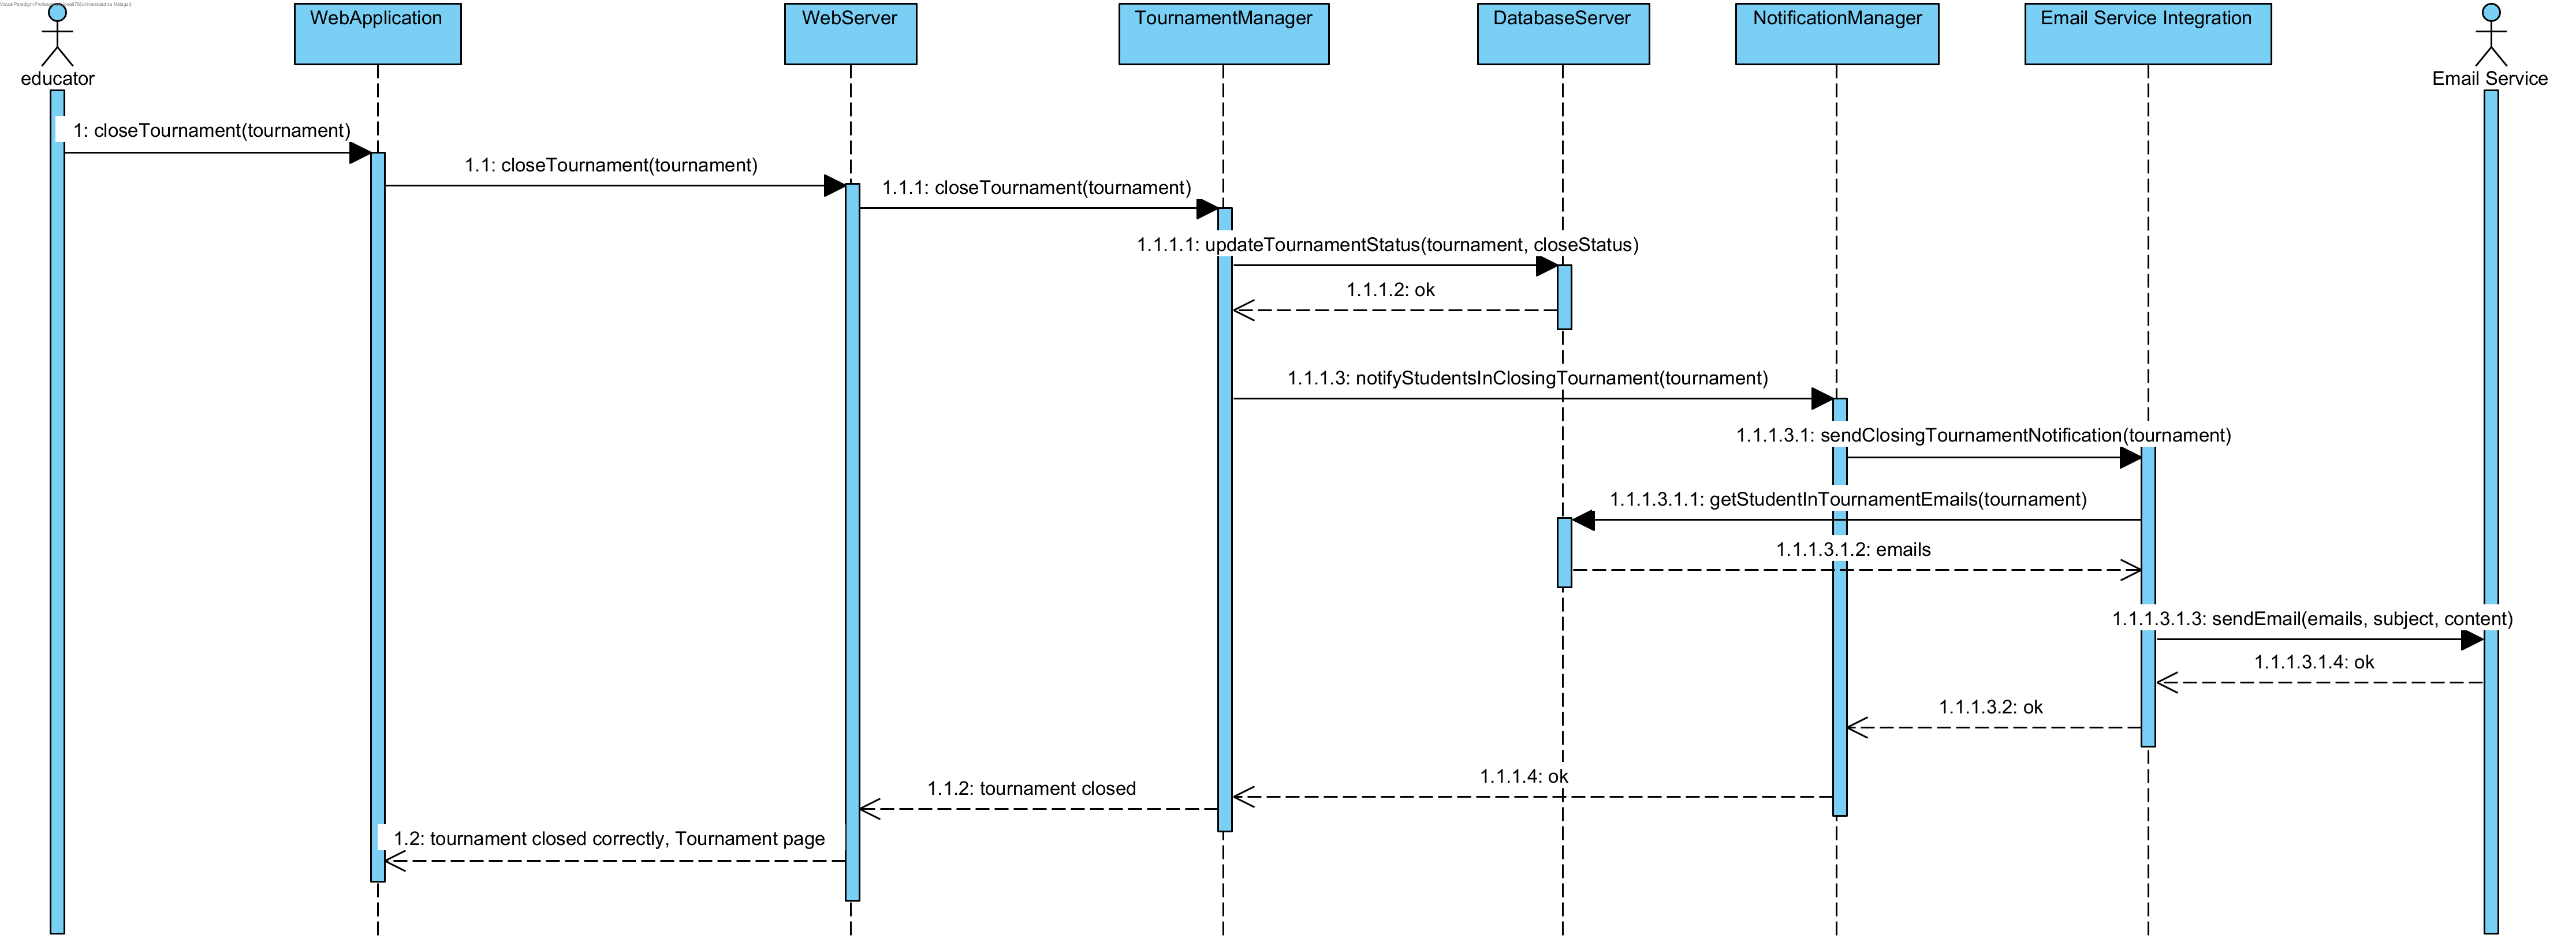
\includegraphics[width=1\textwidth]{images/UseCaseSequenceDiagrams/UC14}
    \caption{Use Case 14}
    \label{fig:UC14}
\end{figure}

\subsubsection*{UC15 - Find Tournament via search}

\begin{figure}[H]
    \centering
    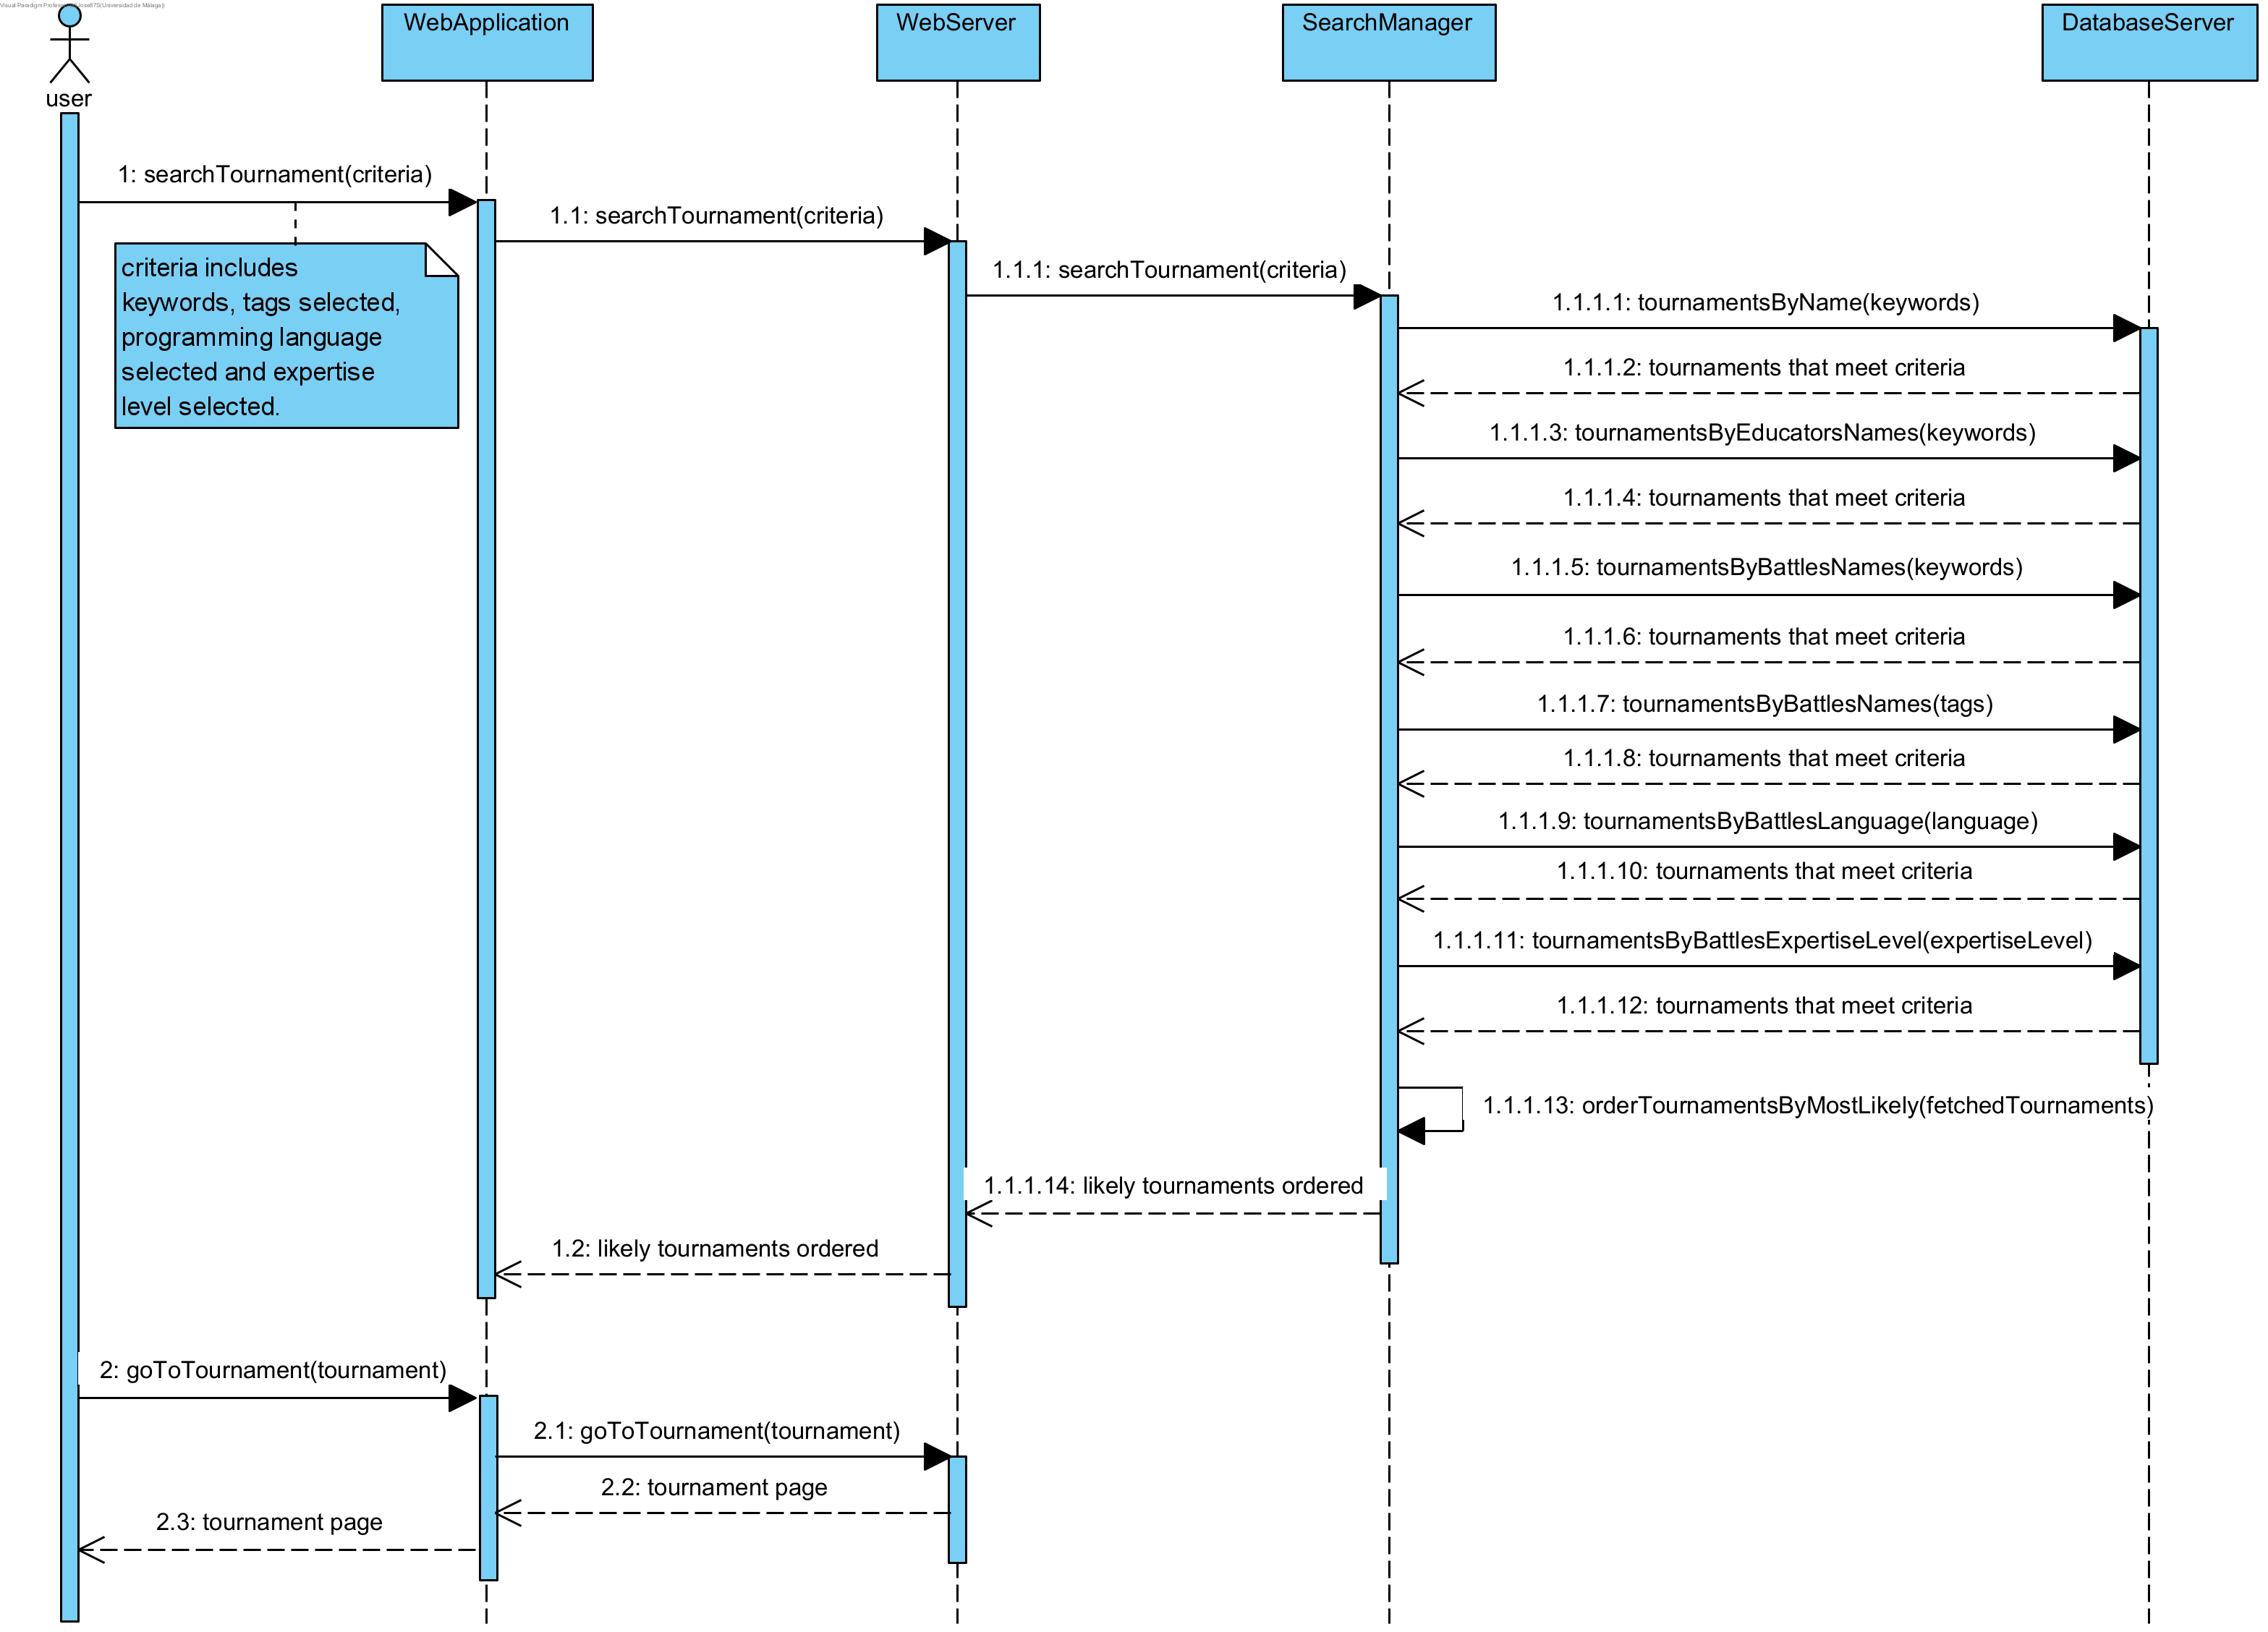
\includegraphics[width=1\textwidth]{images/UseCaseSequenceDiagrams/UC15}
    \caption{Use Case 15}
    \label{fig:UC15}
\end{figure}

\subsubsection*{UC16 - Find Tournament on main page}

\begin{figure}[H]
    \centering
    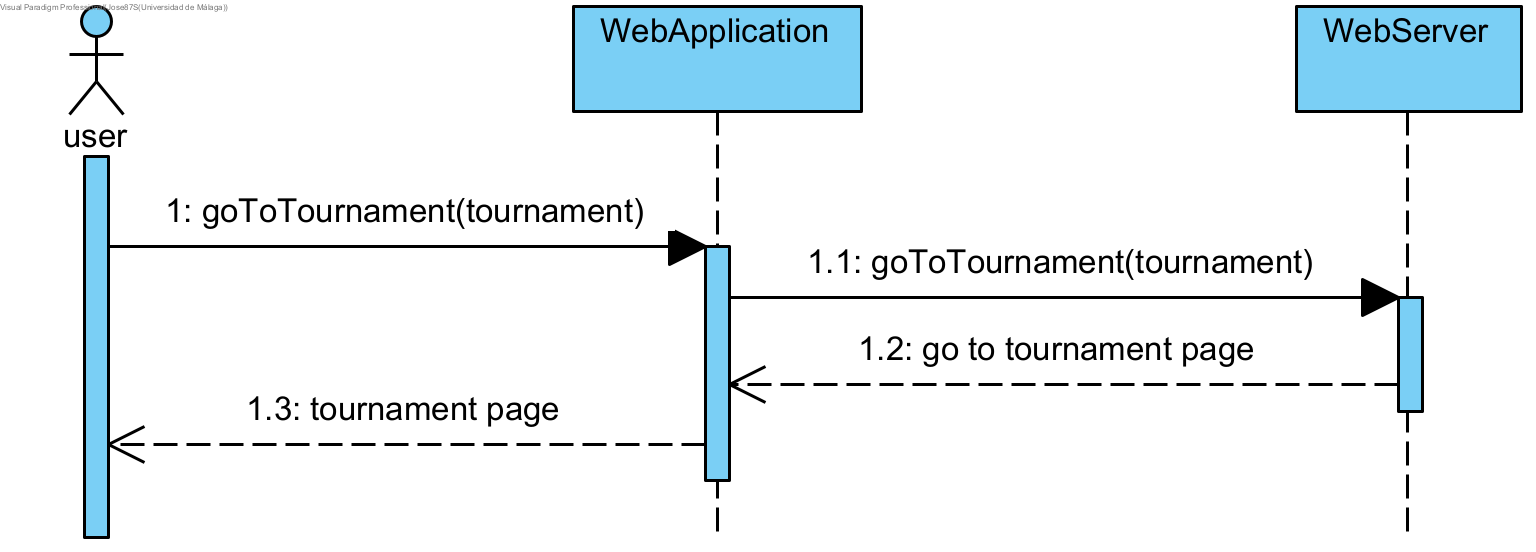
\includegraphics[width=1\textwidth]{images/UseCaseSequenceDiagrams/UC16}
    \caption{Use Case 16}
    \label{fig:UC16}
\end{figure}

\subsubsection*{UC17 - Find Battle on main page or on tournament page}

\begin{figure}[H]
    \centering
    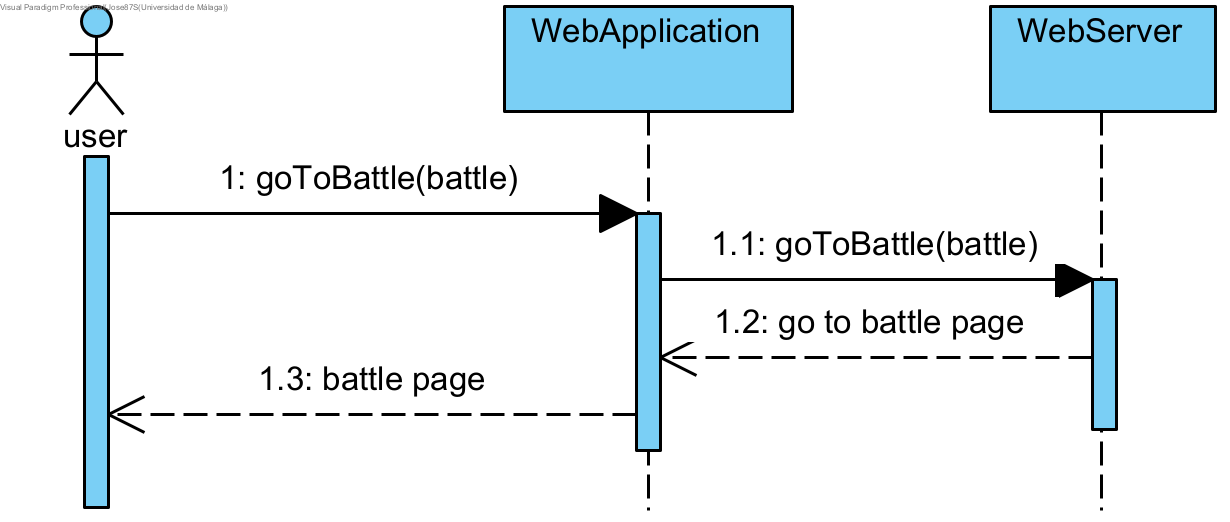
\includegraphics[width=1\textwidth]{images/UseCaseSequenceDiagrams/UC17&18}
    \caption{Use Case 17 and 18}
    \label{fig:UC17and18}
\end{figure}

\newpage

\subsection{Component interfaces}

\paragraph{WebServer:}

\begin{itemize}
    \item void \textbf{loginRequest}(string \textbf{email}, string \textbf{password})
    \item void \textbf{registerRequest}(string \textbf{email}, string \textbf{password}, string \textbf{name}, string \textbf{surname}, string \textbf{gitHubAccount})
    \item void \textbf{retrievePassword}(string \textbf{email})
    \item void \textbf{newPassword}(string \textbf{email}, string \textbf{password})
    \item void \textbf{createTournament}(string \textbf{name}, Date \textbf{registrationDeadline}, Educator \textbf{educator})
    \item void \textbf{inviteEducatorToTournament}(Tournament \textbf{tournament}, Educator \textbf{educatorInvited})
    \item void \textbf{acceptTournamentInvitation}(Tournament \textbf{tournament}, 
    Educator \textbf{educatorInvited})
    \item void \textbf{declineTournamentInvitation}(Tournament \textbf{tournament},
    Educator \textbf{educatorInvited})
    \item void \textbf{createBattle}(Tournament \textbf{tournament}, Educator \textbf{educator}, string \textbf{name}, 
    string \textbf{description}, Date \textbf{registrationDeadline}, Date \textbf{finalSubmissionDeadline}, 
    int \textbf{maxNumberOfParticipants}, int \textbf{minNumberOfParticipants},
    string \textbf{language}, File[] \textbf{testCases}, File[] \textbf{buildAutomationScripts})
    \item void \textbf{registerToTournament}(Tournament \textbf{tournament}, Student \textbf{student})
    \item void \textbf{unregisterFromTournament}(Tournament \textbf{tournament}, Student \textbf{student})
    \item void \textbf{registerToBattle}(Battle \textbf{battle}, Student \textbf{student})
    \item void \textbf{inviteStudentToBattle}(Battle \textbf{battle}, Student \textbf{studentInviting}, Student \textbf{studentInvited})
    \item void \textbf{acceptBattleInvitation}(Battle \textbf{battle}, Student \textbf{studentInviting}, Student \textbf{studentInvited})
    \item void \textbf{unregisterFromBattle}(Battle \textbf{battle}, Student \textbf{student})
    \item void \textbf{seeSubmissions}(Battle \textbf{battle})
    \item void \textbf{setGrade}(StudentTeam \textbf{studentTeam}, float \textbf{grade})
    \item void \textbf{closeBattle}(Battle \textbf{battle})
    \item void \textbf{closeTournament}(Tournament \textbf{tournament})
    \item void \textbf{searchTournament}(string \textbf{keyword}, string[] \textbf{tags}, string \textbf{language}, string \textbf{expertiseLevel})
    \item void \textbf{goToTournament}(Tournament \textbf{tournament})
    \item void \textbf{goToBattle}(Battle \textbf{battle})
\end{itemize}

\paragraph{AuthenticationManager:}

\begin{itemize}
    \item void \textbf{loginRequest}(string \textbf{email}, string \textbf{password})
    \item void \textbf{registerRequest}(string \textbf{email}, string \textbf{password}, string \textbf{name}, string \textbf{surname}, string \textbf{gitHubAccount})
    \item void \textbf{retrievePassword}(string \textbf{email})
    \item void \textbf{newPassword}(string \textbf{email}, string \textbf{password})

\end{itemize}

\paragraph{TournamentManager:}

\begin{itemize}
    \item void \textbf{createTournament}(string \textbf{name}, Date \textbf{registrationDeadline}, Educator \textbf{educator})
    \item void \textbf{inviteEducatorToTournament}(Tournament \textbf{tournament}, Educator \textbf{educatorInvited})
    \item void \textbf{addEducatorToTournament}(Tournament \textbf{tournament}, 
    Educator \textbf{educatorInvited})
    \item void \textbf{addStudent}(Tournament \textbf{tournament}, Student \textbf{student})
    \item void \textbf{unregisterFromTournament}(Tournament \textbf{tournament}, Student \textbf{student})
    \item void \textbf{updateTournamentScores}(Tournament \textbf{tournament}, Battle \textbf{battle})
    \item void \textbf{closeTournament}(Tournament \textbf{tournament})
    
    In addition to these methods, the TournamentManager must also also periodically check if the registration deadline of a tournament has passed, and if so, close the tournament registrations.
    \item void \textbf{monitorDeadlines}()
\end{itemize}

\paragraph{BattleManager:}

\begin{itemize}
    \item void \textbf{createBattle}(Tournament \textbf{tournament}, Educator \textbf{educator}, string \textbf{name}, 
    string \textbf{description}, Date \textbf{registrationDeadline}, Date \textbf{finalSubmissionDeadline},
    int \textbf{maxNumberOfParticipants}, int \textbf{minNumberOfParticipants}, 
    string \textbf{language}, File[] \textbf{testCases}, File[] \textbf{buildAutomationScripts})
    \item void \textbf{registerToBattle}(Battle \textbf{battle}, Student \textbf{student})
    \item void \textbf{inviteStudentToBattle}(Battle \textbf{battle}, Student \textbf{studentInviting}, Student \textbf{studentInvited})
    \item void \textbf{acceptBattleInvitation}(Battle \textbf{battle}, Student \textbf{studentInviting}, Student \textbf{studentInvited})
    \item void \textbf{unregisterFromBattle}(Battle \textbf{battle}, Student \textbf{student})
    \item Map<StudentTeam, File[]> \textbf{seeSubmissions}(Battle \textbf{battle})
    \item void \textbf{setGrade}(StudentTeam \textbf{studentTeam}, float \textbf{grade})
    \item void \textbf{closeBattle}(Battle \textbf{battle})

    In addition to these methods, the BattleManager must also also periodically check if the registration deadline and submission deadline of a battle has passed, and if so, go to the next phase of the battle.
    In the case the registrationDeadline of a Battle has passed, the BattleManager besides closing the registrations, must also create the GitHub repositories for submission and evaluation, uploading to these 
    repositories the test cases and build automation scripts. More specifically, in the submission repository, the BattleManager must setup the GitHub Actions workflow to communicate to the EvaluationManager when a new submission is made.
    On the other hand, in the evaluation repository, the BattleManager must setup the GitHub Actions workflow, test cases and build automation scripts to perform evaluations on uploaded files and communicate to the EvaluationManager the results of these. 
    Besides this, it must also invite the students that registered to the battle to the submission repository.
    \item void \textbf{monitorDeadlines}()
\end{itemize}

\paragraph{NotificationManager:}

\begin{itemize}
    \item void \textbf{newTournamentNotification}(Tournament \textbf{tournament})
    \item void \textbf{inviteEducatorToTournament}(Tournament \textbf{tournament}, Educator \textbf{educatorInvited})
    \item void \textbf{newBattleNotification}(Tournament \textbf{tournament}, Battle \textbf{battle})
    \item void \textbf{inviteStudentToBattle}(Battle \textbf{battle}, Student \textbf{studentInviting}, Student \textbf{studentInvited})
    \item void \textbf{notifyStudentsInClosingBattle}(Battle \textbf{battle})
    \item void \textbf{notifyStudentsInClosingTournament}(Tournament \textbf{tournament})
\end{itemize}

\paragraph{EvaluationManager:}

\begin{itemize}
    \item void \textbf{performEvaluation}(File[] \textbf{submissionFiles}, string \textbf{parentBattleSubmissionRepoUrl}, string \textbf{gitHubAccountStudent})
    \item void \textbf{storeEvaluationResults}(float \textbf{evaluationResult}, int \textbf{StudentTeamId})
\end{itemize}

\paragraph{SearchManager:}

\begin{itemize}
    \item void \textbf{searchTournament}(string \textbf{keyword}, string[] \textbf{tags}, string \textbf{language}, string \textbf{expertiseLevel})
\end{itemize}

\paragraph{GitHub API Integration:}

\begin{itemize}
    \item void \textbf{performEvaluation}(String \textbf{battleEvaluationRepoUrl}, File[] \textbf{submissionFiles}, StudentTeam \textbf{studentTeam})
    \item Map<StudentId, File[]> \textbf{getSubmissionFiles}(Battle \textbf{battle})
\end{itemize}

\paragraph{Email Service Integration:}

\begin{itemize}
    \item void \textbf{sendRecoveryEmail}(string \textbf{email})
    \item void \textbf{sendTournamentNotification}(Tournament \textbf{tournament})
    \item void \textbf{sendTournamentInvitation}(Tournament \textbf{tournament}, Educator \textbf{educatorInvited})
    \item void \textbf{sendBattleNotification}(Tournament \textbf{tournament}, Battle \textbf{battle})
    \item void \textbf{sendBattleInvitation}(Battle \textbf{battle}, Student \textbf{studentInviting}, Student \textbf{studentInvited})
    \item void \textbf{sendClosingBattleNotification}(Battle \textbf{battle})
    \item void \textbf{sendClosingTournamentNotification}(Tournament \textbf{tournament})
\end{itemize}

\subsection{Selected architectural styles and patterns}

\paragraph{3-tier Architecture:}

As explained in the overview, the chosen architecture for the system is a three-tier architecture, a widely adopted
model for developing scalable and maintainable web applications. This architectural 
style divides the application into three interconnected layers: presentation, application,
and data, with the addition of the external services like GitHub and email services.

\paragraph{Model-View-Controller:}

The Model-View-Controller (MVC) is a software architectural pattern that separates an application into three main logical components: the model, the view, and the controller. Each of these components are built to handle specific development aspects of an application. MVC is one of the most frequently used industry-standard web development framework to create scalable and extensible projects.
In the case of this system, it is used to separate the presentation layer from the application layer.

\paragraph{RESTful API:}

REST stands for Representational State Transfer. It is a software architectural style that defines a set of constraints to be used for creating web services. Web services that conform to the REST architectural style, called RESTful web services, provide interoperability between computer systems on the Internet. RESTful web services allow the requesting systems to access and manipulate textual representations of web resources by using a uniform and predefined set of stateless operations. In the case of this system, it is used to define the communication between the presentation layer and the application layer.

\subsection{Other design decisions}

\paragraph{Entity Relationship Diagram:}

The structure defined for the database is as follows:

\begin{figure}[H]
    \centering
    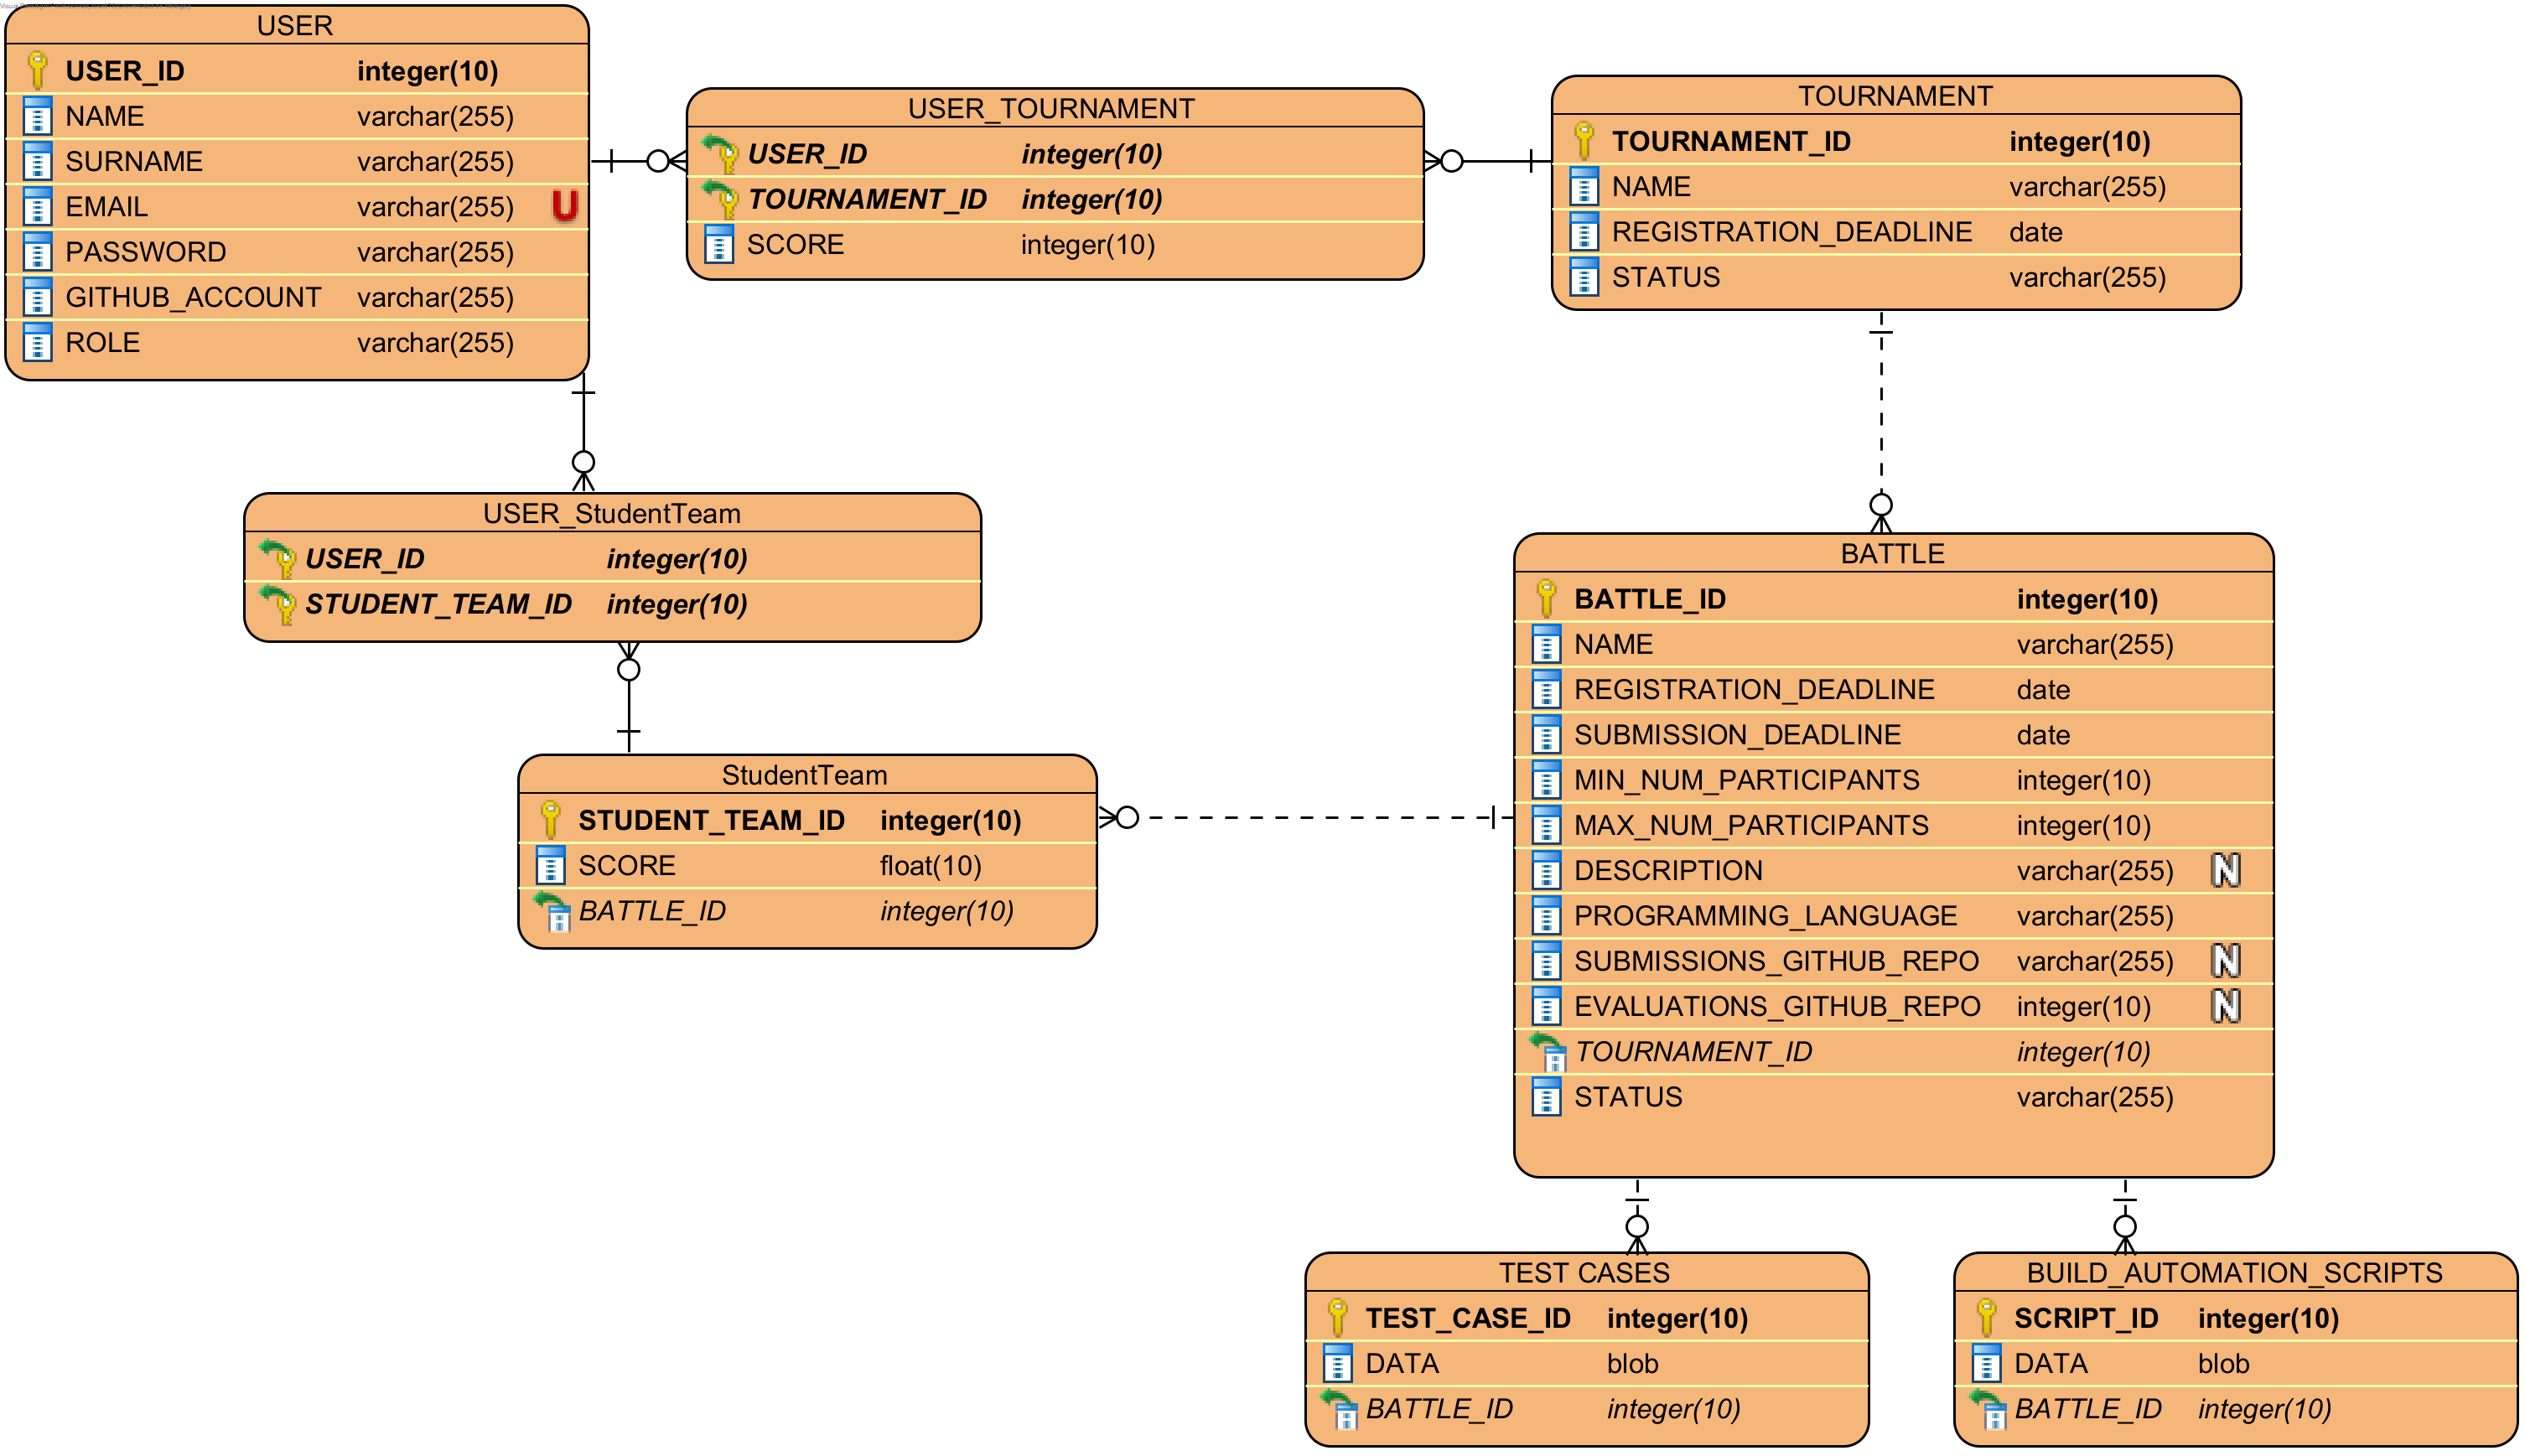
\includegraphics[width=1\textwidth]{images/EntityRelationshipDiagram.png}
    \caption{Entity Relationship Diagram}
    \label{fig:EntityRelationshipDiagram}
\end{figure}

Also, in order to prevent a single point of failure in the database, it is replicated in a master-slave configuration.

% 3. USER INTERFACE DESIGN
\section{USER INTERFACE DESIGN}

\subsection{Mockups}

\paragraph{Homepage for all users:}

\begin{figure}[H]
    \centering
    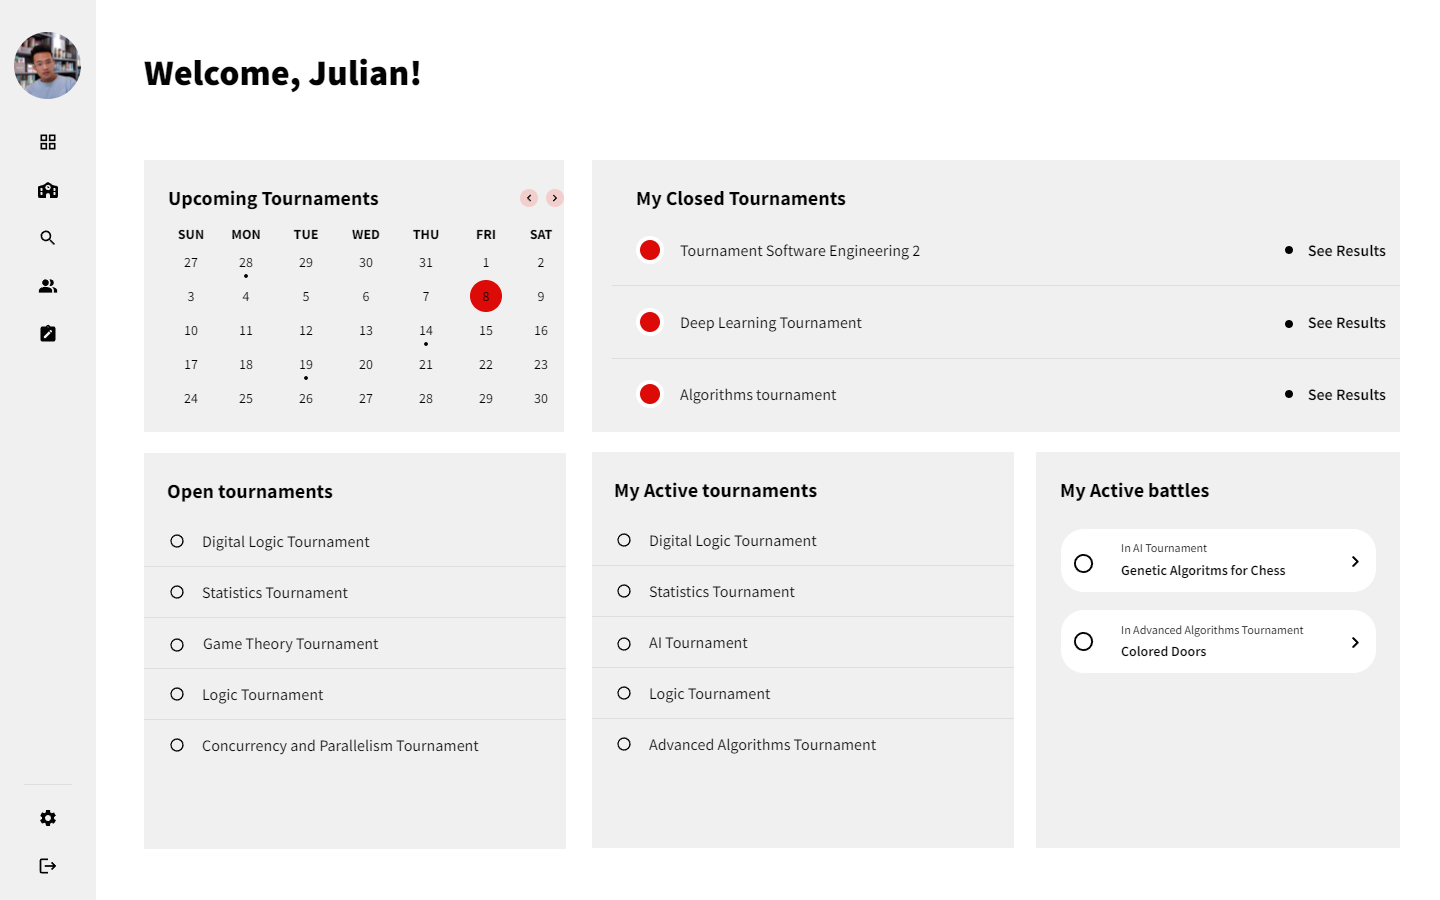
\includegraphics[width=1\textwidth]{images/UI/Homepage.png}
    \caption{Homepage}
    \label{fig:Homepage}
\end{figure}

On this screen, both students and educators can see the tournaments and battles 
they are a part of, the closed tournaments in which they participated and open 
tournaments they can register to or be invited to respectively. From this screen, they
can travel to the tournament or battle page by clicking on the respective card. If there
are more tournaments or battles than the ones that can be shown, the user can scroll down
on each of the tabs to see more. There is also a calendar that shows the important dates
of both the upcoming tournaments and battles and the ones that are currently happening and
the user is a part of. Users can go to the search enviornment from here. 
Educators can go to the tournament creation page from here as well.

\paragraph{Tournament Page for Students before Registration Deadline Expires:}

\begin{figure}[H]
    \centering
    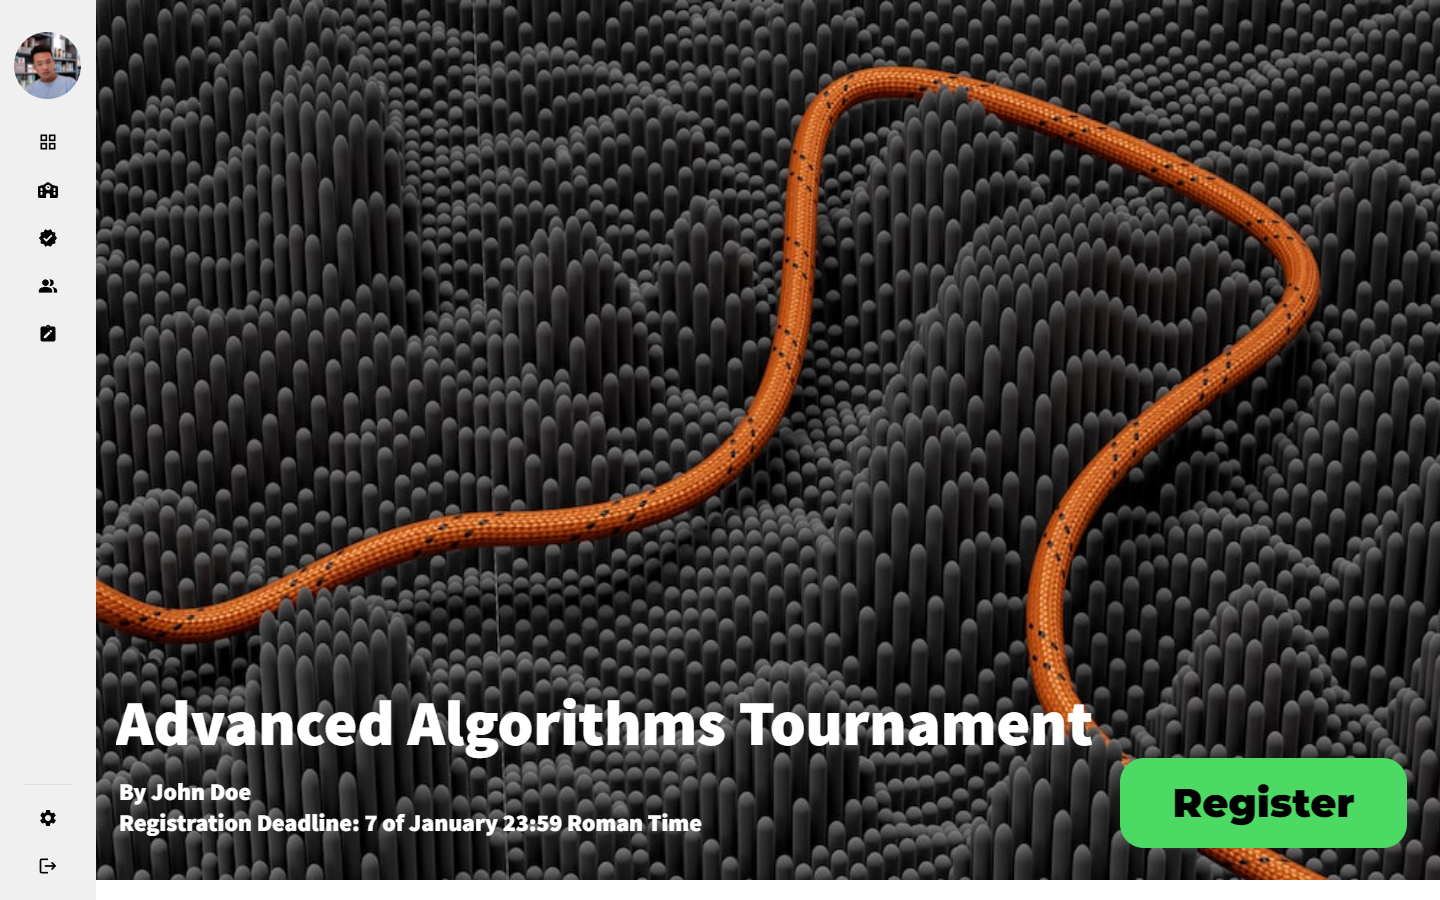
\includegraphics[width=1\textwidth]{images/UI/Tournament Page before Registration Deadline Student not registered.png}
    \caption{Tournament Page for Students before Registration Deadline expires}
    \label{fig:TournamentPageForStudentsBeforeRegistrationDeadline}
\end{figure}

On this screen, students can see the name and registration deadline of the tournament.If the student
is not registered, they can register to thebattle. If the student is already registered, they can 
unregister from the battle.

\paragraph{Active Tournament Page for Student:}

\begin{figure}[H]
    \centering
    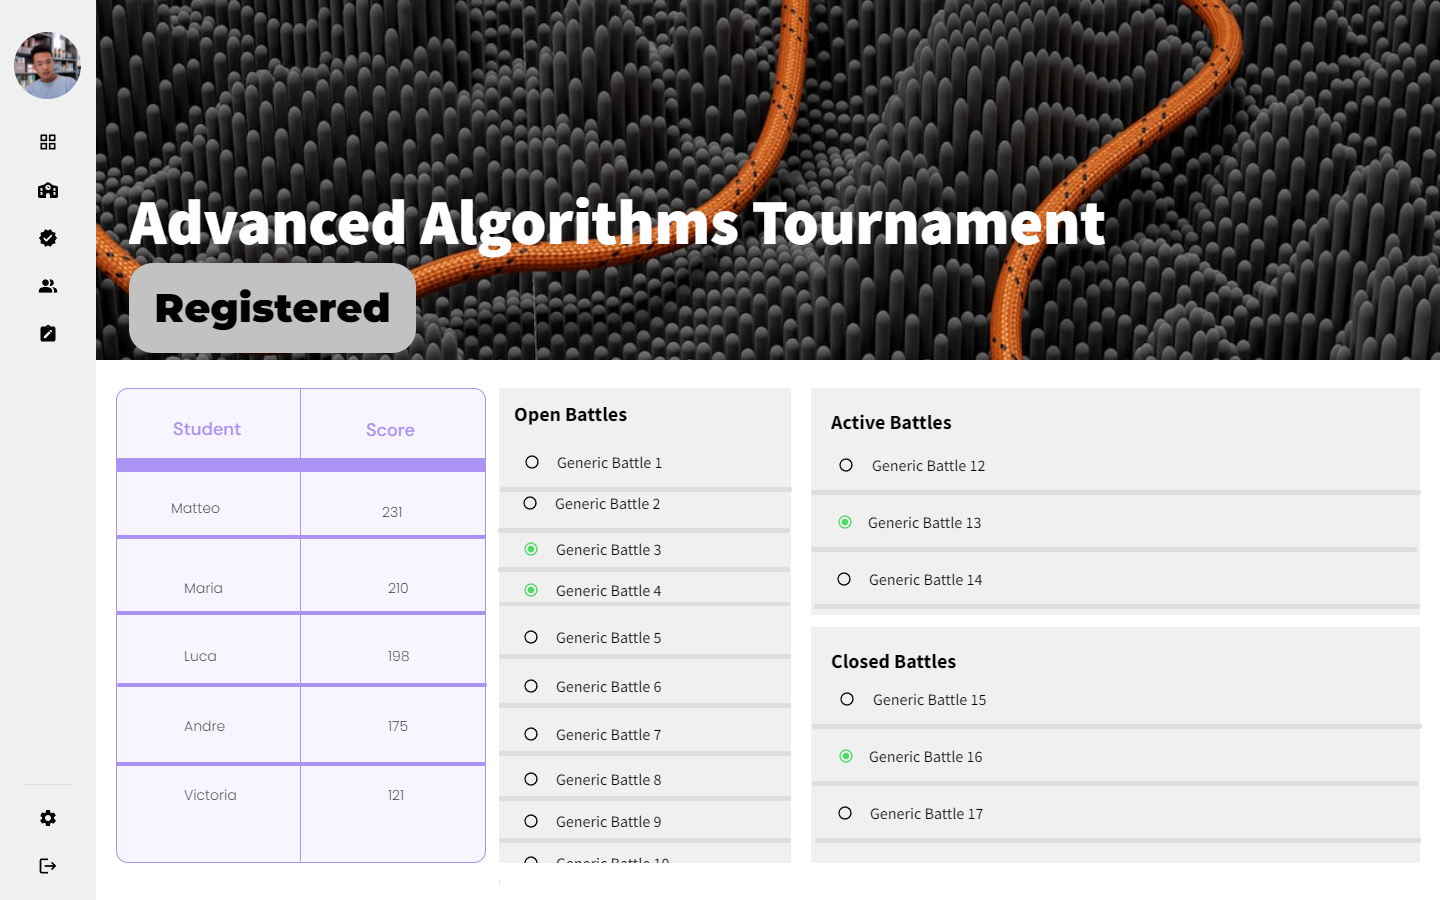
\includegraphics[width=1\textwidth]{images/UI/Tournament Page Active.png}
    \caption{Active Tournament Page for Students}
    \label{fig:ActiveTournamentPageForStudents}
\end{figure}

On this screen, students can seet the leaderboard, open, active and closed battles of that tournament.
If the student seeing the page is registered to the tournament it will be shown with a non-clickable indicator.
If the student is registered to a battle, it will be shown with a green indicator. Students can go to any
of the tournaments by clicking on the respective name. 

\paragraph{Active Tournament Page for Educator:}

\begin{figure}[H]
    \centering
    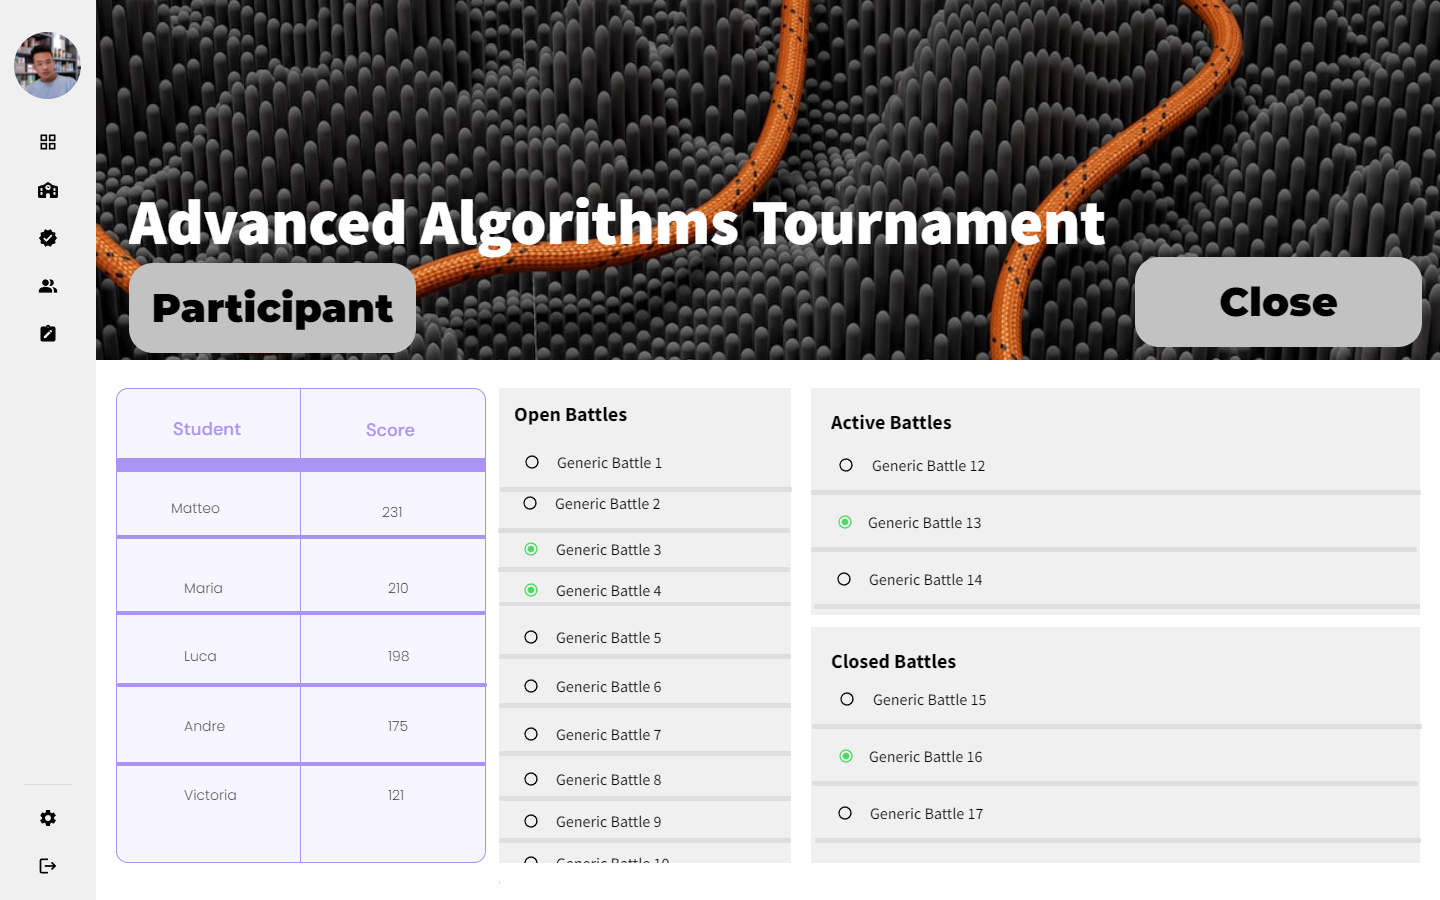
\includegraphics[width=1\textwidth]{images/UI/Tournament Page Active Educator.png}
    \caption{Active Tournament Page for Educator}
    \label{fig:ActiveTournamentPageForEducator}
\end{figure}

On this screen, educators can seet the leaderboard, open, active and closed battles of that tournament.
If the educator is the owner or is a participant of the tournament, this will be shown with a non-clickable indicator.
If the educator is the owner of a battle, a close tournament button will be shown. This button is unavailable
if there are open or active battles in the tournament.
If a educator is the owner of a battle, it will be shown with a green indicator. Educators can go to any
of the battles in the tournament by clicking on the respective name.
From here the educator can also create battles for the tournament.

\paragraph{Open Battle Page:}

\begin{figure}[H]
    \centering
    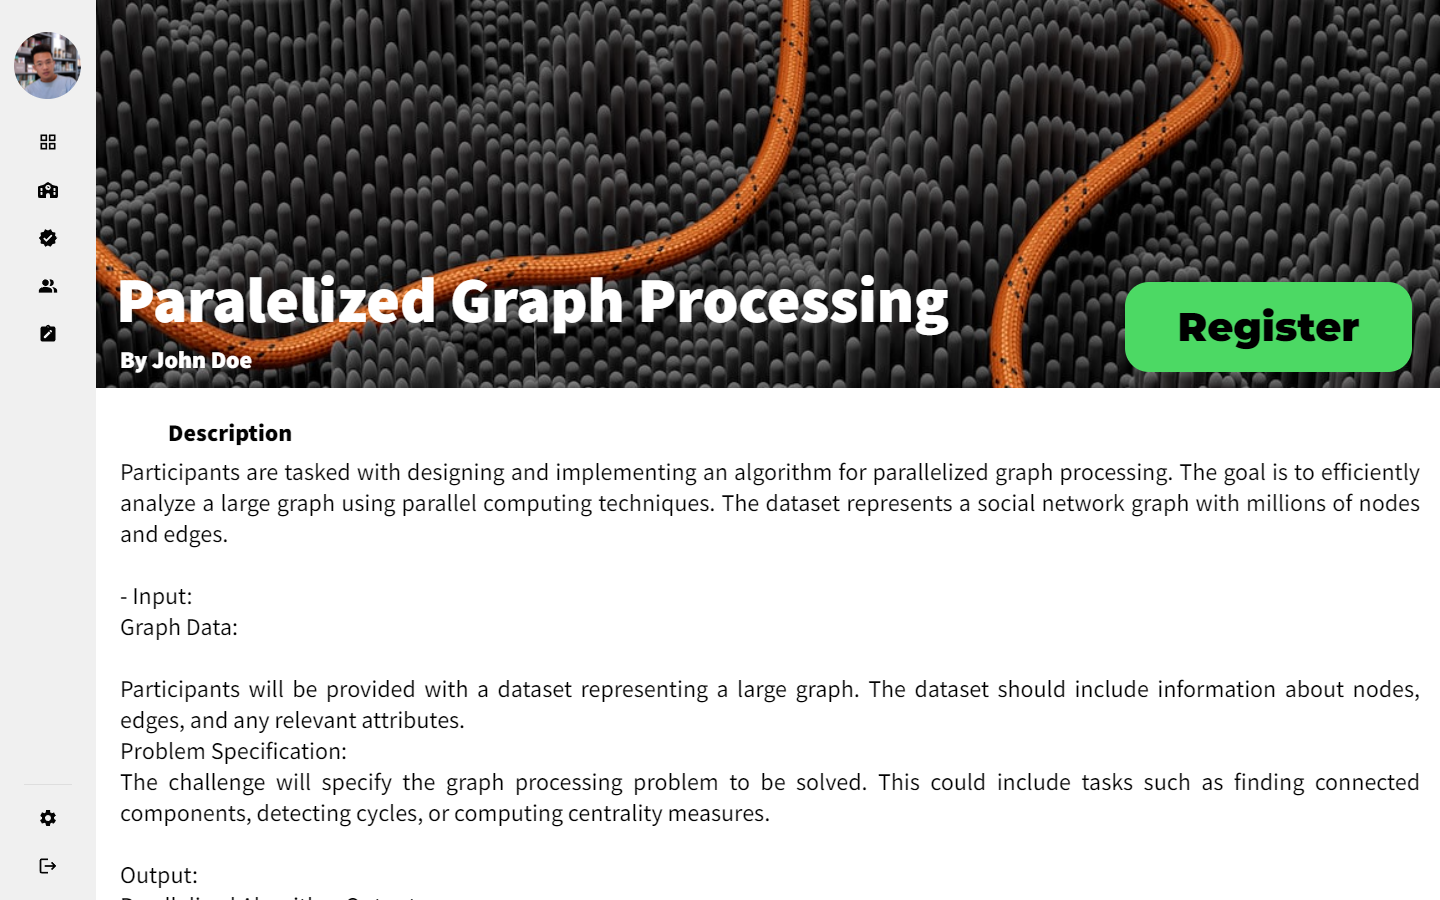
\includegraphics[width=1\textwidth]{images/UI/Battle Screen before Registration Deadline Student not registered.png}
    \caption{Open Battle Page}
    \label{fig:OpenBattlePage}
\end{figure}

On this screen, users can see the details of the battle, such as the description, the
language and other information. Additionally, if the user is a student and if the student is 
registered to the tournament the battle belongs to and is not registered to the battle, they can register it. 
If the student is already registered to the battle, they can unregister from the battle. Also, if the student
is registered, they can invite other students to the battle. 

\paragraph{Active or Closed Battle Page:}

\begin{figure}[H]
    \centering
    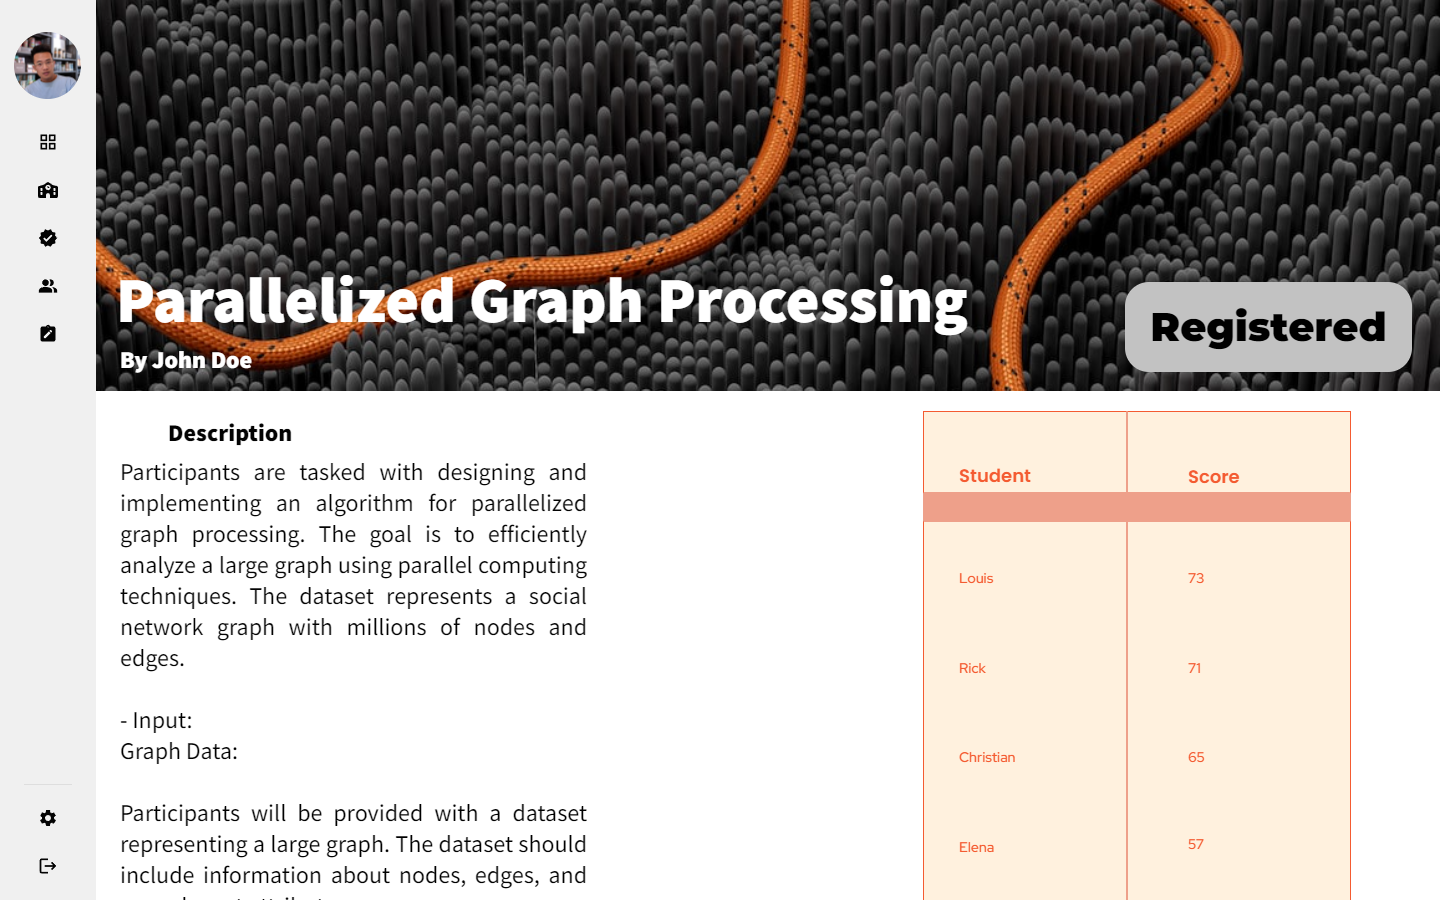
\includegraphics[width=1\textwidth]{images/UI/Battle Screen Active Student.png}
    \caption{Active Battle Page}
    \label{fig:ActiveBattlePage}
\end{figure}

On this screen, users can see the details of the battle, such as the description, the
language and the leaderboard. Additionally, if the user is a student and registered to the battle,
it displays this information.

The different tournament and battle pages are located on the same URL for the same tournament or battle.
The differences shown on the UI are dependant of the status of the tournament or battle and the type of user.

\paragraph{Tournament Creation Page:}

\begin{figure}[H]
    \centering
    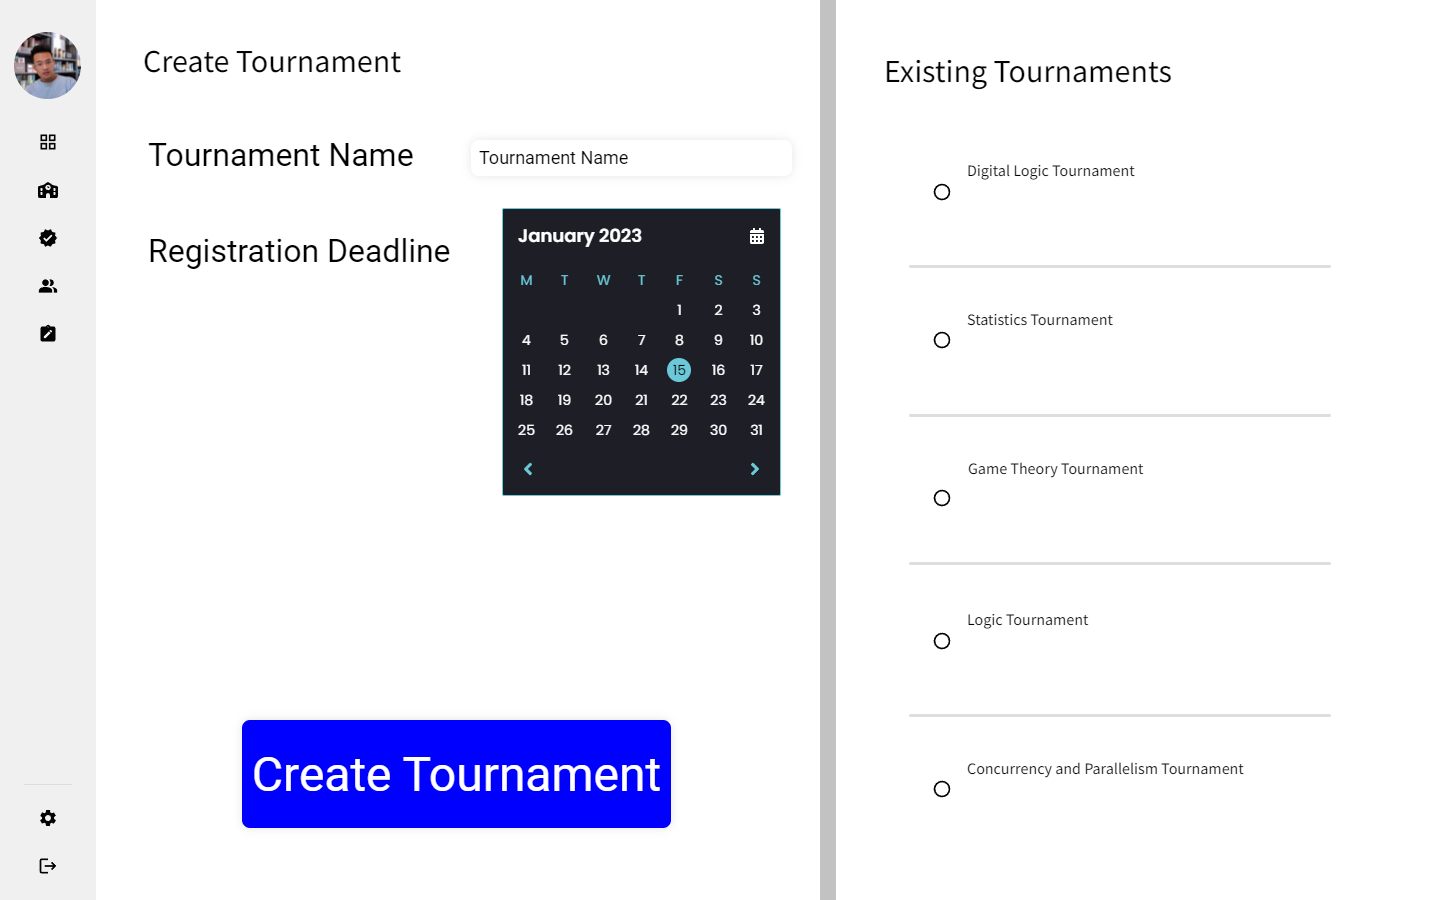
\includegraphics[width=1\textwidth]{images/UI/Create Tournament.png}
    \caption{Tournament Creation Page}
    \label{fig:TournamentCreationPage}
\end{figure}

\paragraph{Battle Creation Page:}

\begin{figure}[H]
    \centering
    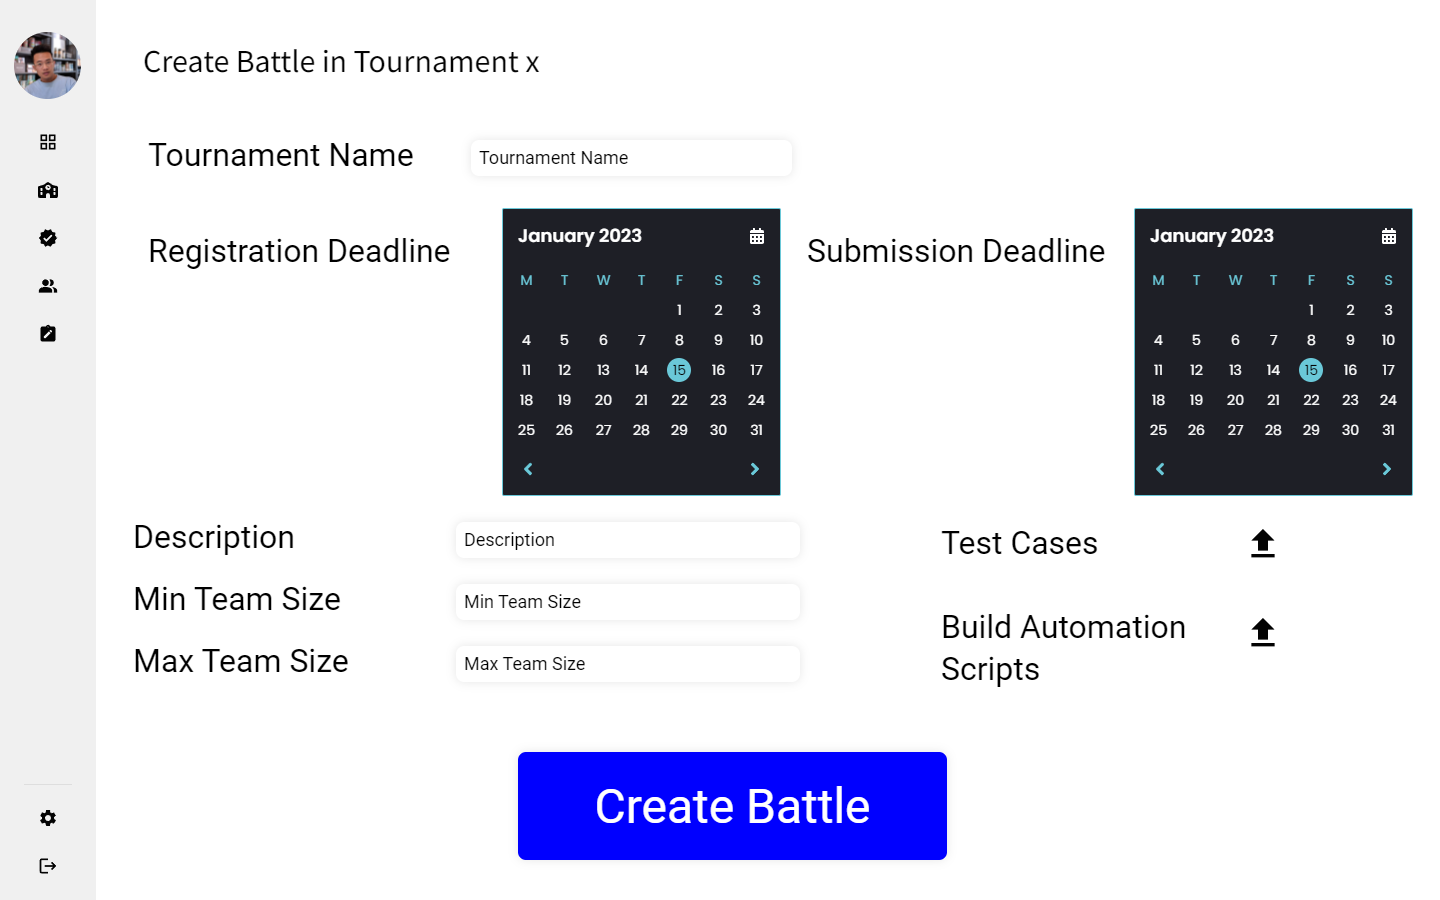
\includegraphics[width=1\textwidth]{images/UI/Create Battle.png}
    \caption{Battle Creation Page}
    \label{fig:BattleCreationPage}
\end{figure}

On this screen, educators can create a Battle by filling the form with the all the necessary information.

\paragraph{Search Enviornment:}

\begin{figure}[H]
    \centering
    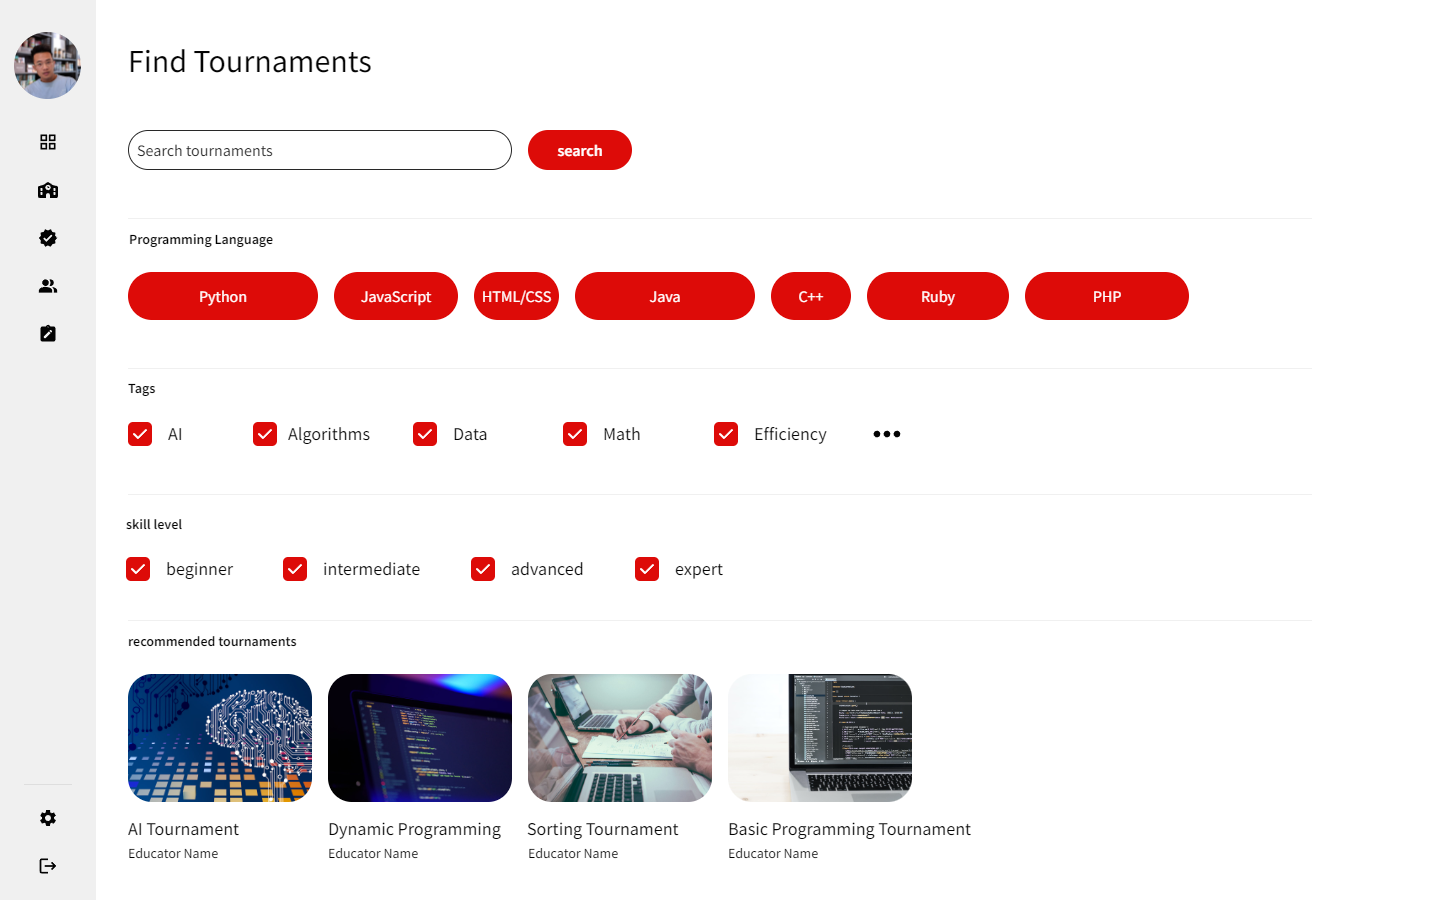
\includegraphics[width=1\textwidth]{images/UI/Search.png}
    \caption{Search Enviornment}
    \label{fig:SearchEnviornment}
\end{figure}

On this screen, users can look for tournaments according to keywords, language, tags and expertise level.
The results are shown in a list, and the user can click on any of the tournaments to go to the tournament page.

Other screens like login, register, password recovery, etc. are not shown as they are standard and similar to other applications.

\subsection{Flowchart}

\begin{figure}[H]
    \centering
    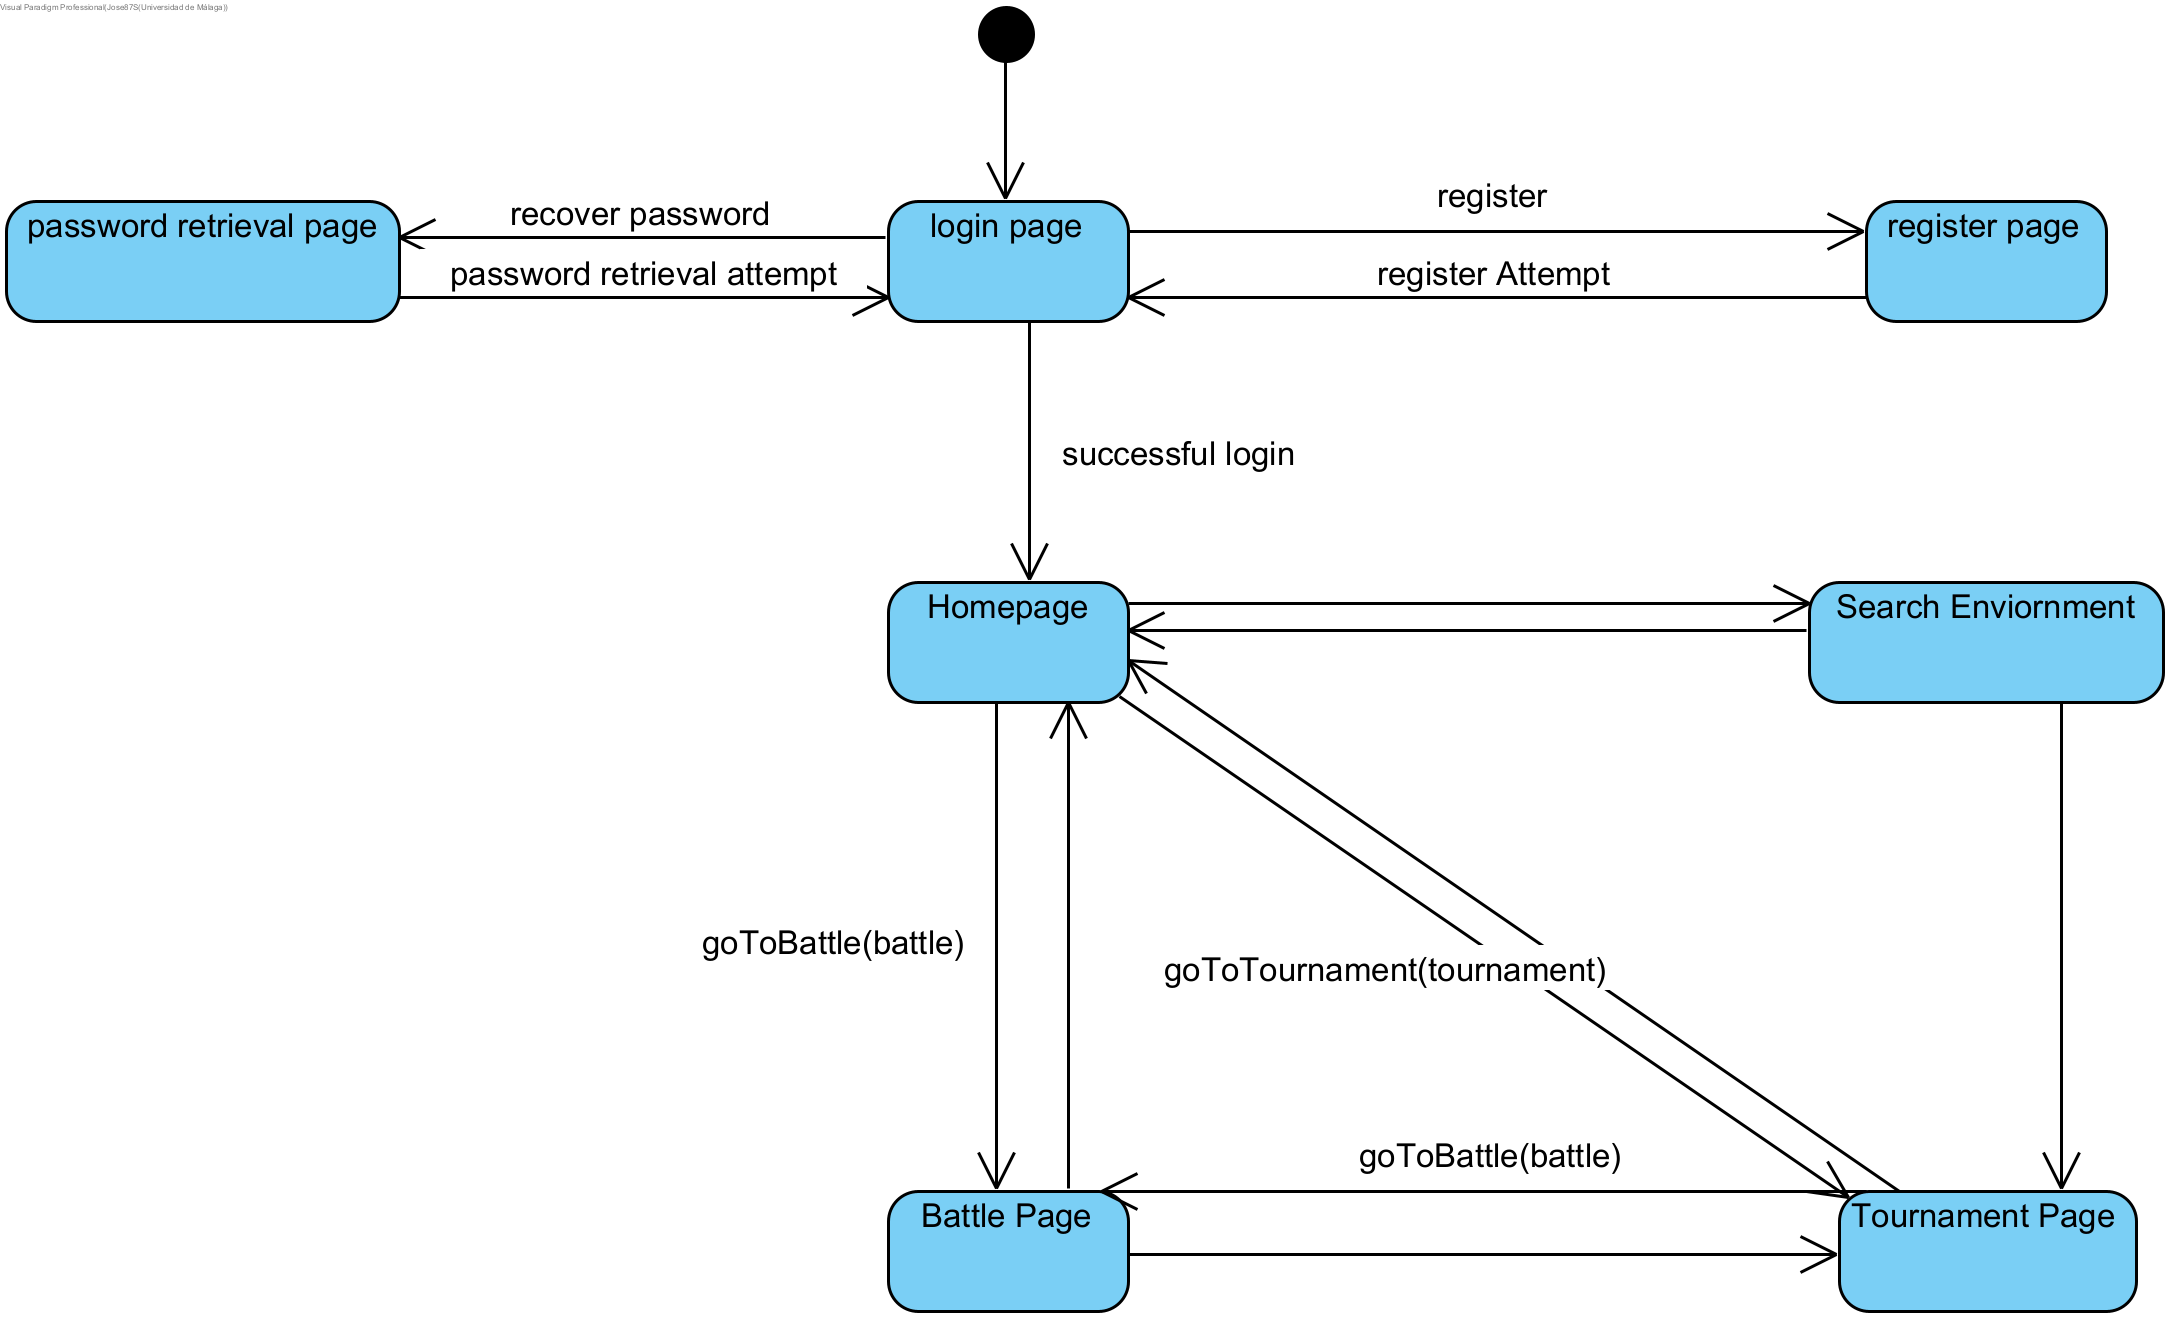
\includegraphics[width=1\textwidth]{images/UI/UserInterfaceFlowchart.png}
    \caption{User Interfaces Flowchart}
    \label{fig:UserInterfacesFlowchart}
\end{figure}

This diagram shows the flow of the user interfaces of the system on a normal execution. There are other
possible flows, such as entering to specific pages for accepting invitations or new password creation, but
these are only accessible via email link and are not shown here.

% 4. REQUIREMENTS TRACEABILITY
\section{REQUIREMENTS TRACEABILITY}

The following is the list of requirements specified in the RASD document. For each requirement or group of them,
there is a group of components and some functionalities the components possess that fulfill the requirements. These 
components and functionalities are declared just below the group of requirements they fulfill.

\begin{itemize}

    \subsubsection*{Authentication}

    \item \textbf{R1:} At any time, The system shall allow users to register.
    \item \textbf{R2:} At any time, The system shall allow user to login. 
    \item \textbf{R4:} At any time, two accounts with the same email may not exist.
    \item \textbf{R5:} At any time, an account may not have a password without a number and more than 8 characters.
    
    All the previous requirements are fulfilld by the following functionalities:

    \textbf{Web Application:} Register Page

    \textbf{Web Server:} registerRequest

    \textbf{AuthenticationManager:} registerRequest

    \item \textbf{R3:} At any time, The system shall allow users to try to recover their password by sending a password recovery email.

    \textbf{Web Application:} Recover Password Page

    \textbf{Web Server:} retrievePassword

    \textbf{AuthenticationManager:} retrievePassword

    \textbf{Email Services Integration:} sendRecoveryEmail

    \subsubsection*{Tournament and Battle Creation}

    \item \textbf{R6:} At any time, The system shall allow logged in educators to create tournaments.
    \item \textbf{R7:} When creating a tournament, the educator that is doing so must be able to set the registration deadline.
    \item \textbf{R8:} When creating a tournament, the educator that is doing so must be able to set a name.
    \item \textbf{R9:} When creating a tournament, the parameters being set must be valid. This means that the registration deadline must be in the future and the name must be a non empty string.
    
    \textbf{Web Application:} Create Tournament Page

    \textbf{Web Server:} createTournament

    \textbf{TournamentManager:} createTournament

    \item \textbf{R10:} After the creation of a tournament, the system shall notify all the students that a tournament has been created.

    \textbf{NotificationManager:} newTournamentNotification

    \textbf{Email Services Integration:} sendTournamentNotification

    \item \textbf{R11:} At any time, The system shall allow logged in educators to invite other educators to tournaments they own and logged in educators that have been invited should be able to accept this invitations.
    
    \textbf{Web Application:} Tournament Page

    \textbf{Web Server:} inviteEducatorToTournament, acceptTournamentInvitation, declineTournamentInvitation

    \textbf{TournamentManager:} inviteEducatorToTournament, addEducatorToTournament

    \textbf{NotificationManager:} inviteEducatorToTournament

    \textbf{Email Services Integration:} sendTournamentInvitation

    \item \textbf{R12:} At any time, The system shall allow logged in educators to create battles inside tournaments they are a part of.
    \item \textbf{R13:} When creating a battle, the educator that is doing so must be able to upload a description of the problem.
    \item \textbf{R14:} When creating a battle, the educator that is doing so must be able to choose the programming language.
    \item \textbf{R15:} When creating a battle, the educator that is doing so must be able to set the registration deadline.
    \item \textbf{R16:} When creating a battle, the educator that is doing so must be able to set the final submission deadline.
    \item \textbf{R17:} When creating a battle, the educator that is doing so must be able to set the minimum and maximum number of participants per group.
    \item \textbf{R18:} When creating a battle, the educator that is doing so must be able to upload the test cases that will be used to evaluate the students' code.
    \item \textbf{R19:} When creating a battle, the educator that is doing so must be able to upload the build automation scripts that will be used to evaluate the students' code.
    \item \textbf{R20:} When creating a battle, the parameters being set must be valid. This means that the registration deadline must be in the future, the final submission deadline must be after the registration deadline, the minimum number of participants per group must be greater than 0, the maximum number of participants per group must be greater than or equal to the minimum number of participants per group, the programming language must be a valid programming language, the description of the problem must be a non empty string, the test cases must be a valid set of test cases and the build automation scripts must be a valid set of build automation scripts. This last two vary according to the programming language.

    \textbf{Web Application:} Create Battle Page

    \textbf{Web Server:} createBattle

    \textbf{BattleManager:} createBattle

    \item \textbf{R21:} After the creation of a battle, the system shall notify all students that are registered to the tournament the battle belongs to that a battle has been created.

    \textbf{NotificationManager:} newBattleNotification

    \subsubsection*{Tournament and Battle Registration}

    \item \textbf{R22:} At any time, The system shall allow logged in students to register for tournaments before the registration deadline of said tournament if they are yet not registered.
    \item \textbf{R23:} At any time, The system shall allow logged in students to cancel their registration for tournaments they belong to before the registration deadline of said tournament.
    
    \textbf{Web Application:} Tournament Page

    \textbf{Web Server:} registerToTournament, unregisterFromTournament

    \textbf{TournamentManager:} registerToTournament, unregisterFromTournament

    \item \textbf{R24:} At any time, The system shall allow logged in students to register for battles of a tournament they belong to before the registration deadline of said battle if they are not registered.
    \item \textbf{R25:} When registering for a battle, the student that is doing so must be able to invite other students to the battle.
    \item \textbf{R26:} At any time, The system shall allow logged in students to accept invitations to battles of a tournament they belong to before the registration deadline of said battle.
    \item \textbf{R27:} At any time, The system shall allow logged in students to cancel their registration for battles they belong to before the registration deadline of said battle.
    
    \textbf{Web Application:} Battle Page

    \textbf{Web Server:} registerToBattle, inviteStudentToBattle, acceptBattleInvitation, unregisterFromBattle

    \textbf{BattleManager:} registerToBattle, inviteStudentToBattle, acceptBattleInvitation, unregisterFromBattle

    \textbf{NotificationManager:} inviteStudentToBattle

    \subsubsection*{Leaderboards}

    \item \textbf{R28:} At any time, The system shall allow logged in users to see the leaderboard of any tournament.
    \item \textbf{R29:} At any time, The system shall allow logged in users to see the leaderboard of any battle.
    
    \textbf{Web Application:} Tournament Page, Battle Page

    \subsubsection*{Submissions and Evaluations}

    \item \textbf{R30:} When the registration deadline of a battle expires, the system shall create a GitHub repository for the battle that the students should fork to make submissions. This repository should have the GitHub Actions workflow set up to receive notifications from GitHub when a commit is pushed to the main branch. This way, when students fork the GitHub actions of the fork will be already set up.
    \item \textbf{R31:} When the registration deadline of a battle expires, the system shall create a GitHub repository with the appropriate files, including the automation scripts and test cases files for the battle that the system will use to evaluate the submissions of the students.
    \item \textbf{R32:} When the registration deadline of a battle expires, the system shall send invitations to the GitHub repository used for submissions of the battle to the students that registered for it.
    
    \textbf{BattleManager:} monitorDeadlines

    \item \textbf{R33:} At any time, the system should be able to receive notifications from GitHub that a commit has been pushed to the main branch of one of the forked repositories of the battle.
    \item \textbf{R34:} The system should be able to pull the latest sources from the forked repository of the battle that the notification came from.
    
    \textbf{EvaluationManager:} performEvaluation

    \item \textbf{R35:} The system should be able to upload the latest sources from the forked repository of the battle that the notification came from, to the evaluation repository of the battle.
    
    \textbf{EvaluationManager:} performEvaluation

    \textbf{GitHub API Integration:} performEvaluation

    \item \textbf{R36:} The system should be able to receive the results of the evaluation from the evaluation repository of the battle.
    \item \textbf{R37:} The system should be able to update the leaderboard of the battle with the results of the evaluation and the timeliness of the submission.
    
    \textbf{EvaluationManager:} storeEvaluationResults
    
    \subsubsection*{Manual Evaluations}

    \item \textbf{R38:} Once the final submission deadline of a battle expires, the system shall allow the educator that created the battle to manually evaluate the submissions of the students.
    
    \textbf{Web Application:} Battle Page, Submissions Page

    \textbf{Web Server:} seeSubmissions, setGrade

    \textbf{BattleManager:} seeSubmissions, setGrade

    \textbf{GitHub API Integration:} getSubmissionFiles
    
    \subsubsection*{Battle and Tournament Closing}

    \item \textbf{R39:} Once the educator that created the battle finishes manually evaluating the submissions of the students and closes the battle, the system shall notify all the students that participated in the battle that the final results have been published.
    \item \textbf{R40:} Once the educator that created the battle finishes manually evaluating the submissions of the students and closes the battle, the system shall update the leaderboard of the tournament that the battle belongs to by adding the score that each student got on the battle to their score on the rest of the battles of the tournament that they have participated in.
    
    \textbf{Web Application:} Battle Page

    \textbf{Web Server:} closeBattle

    \textbf{BattleManager:} closeBattle

    \textbf{NotificationManager:} notifyStudentsInClosingBattle

    \textbf{Email Services Integration:} sendClosingBattleNotification

    \item \textbf{R41:} At any time, if there are no open battles in a tournament, the system shall allow the owner of the tournament to close it.
    \item \textbf{R42:} Once the owner of a tournament closes it, the system shall update the leaderboard of the tournament and notify all the students that participated in it that the tournament has ended.
    
    \textbf{Web Application:} Tournament Page

    \textbf{Web Server:} closeTournament

    \textbf{TournamentManager:} closeTournament

    \textbf{NotificationManager:} notifyStudentsInClosingTournament

    \textbf{Email Services Integration:} sendClosingTournamentNotification

    \subsubsection*{Search system}

    \item \textbf{R43:} At any time, the system shall allow logged in users to search for tournaments. The system should return the tournaments that match the search criteria. This criteria is given by the keywords the user searched for, the tags the user selected, the programming language the user selected and the difficulty level the user selected.
    
    \textbf{Web Application:} Search Page

    \textbf{Web Server:} searchTournament

    \textbf{SearchManager:} searchTournament
    
    \item \textbf{R44:} At any time, the system shall display to students the tournaments they are registered to.
    \item \textbf{R45:} At any time, the system shall display to students the battles they are registered to.
    \item \textbf{R46:} At any time, the system shall display to educators the tournaments own or are a part of.
    \item \textbf{R47:} At any time, the system shall display to educators the battles they own.
    
    \textbf{Web Application:} Homepage

    \item \textbf{R48:} At any time, the system shall display to users that are inside a tournament the battles of that tournament.
    
    \textbf{Web Application:} Tournament Page


\end{itemize}


% 5. IMPLEMENTATION, INTEGRATION AND TEST PLAN
\section{IMPLEMENTATION, INTEGRATION AND TEST PLAN}



% 6. EFFORT SPENT
\section{EFFORT SPENT}

% 7. REFERENCES
\section{REFERENCES}


\end{document}
